\documentclass[a4paper]{report}

% Number of "levels" the label can reference. Default is 2.
\setcounter{secnumdepth}{3}


\usepackage[english, science, titlepage]{ku-frontpage}

\usepackage[latin1]{inputenc}
\usepackage{palatino}
% \usepackage[usenames]{color}

\usepackage{hyperref}

\usepackage{chngpage}
\usepackage{graphicx}

\usepackage{booktabs}
\usepackage{multirow}
\usepackage[nounderscore]{syntax}
\setlength{\grammarparsep}{0.25cm}
\setlength{\grammarindent}{3.5cm}

\usepackage[]{algorithm2e}
\usepackage{varwidth}

\usepackage{subcaption}

\usepackage{setspace}


\usepackage{todonotes}


\usepackage{listings}
\usepackage[outputdir=.tmp]{minted}
% \usepackage[cache=false]{minted}
\setminted{frame=lines,linenos=true,framesep=2mm,fontsize=\small}


% \usepackage[outputdir=.tmp,chapter,newfloat=true,cache=true]{minted}
% \setminted{fontsize=\scriptsize, frame=single, framesep=2mm, autogobble}
% \usemintedstyle{default}
\usepackage{times}

\usepackage{amsmath}
\usepackage{amssymb}
\normalfont
%\usepackage[T1]{fontenc}
\renewcommand{\ttdefault}{cmtt}
\usepackage{xcolor}
\usepackage{booktabs,siunitx}
\usepackage[font=small]{caption}

\usepackage{parcolumns}

% NOTE: The margins become wider just by including the geometry package
\usepackage{geometry}
\geometry{
%  % a4paper,
%  % total={170mm,257mm},
%  % left=20mm,
 top=30mm,
 bottom=40mm
 }

% \usepackage{url}
\usepackage{pgfplots}
\usepackage{tikz}


% \usepackage[%
%   backend=biber,
%   style=numeric,
%   maxnames=2,
%   minnames=1,
%   maxbibnames=99,
%   firstinits,
%   uniquename=init,
%   backref=true]{biblatex} % TODO: adapt citation style
%   %maxcitenames=2,
%
% \AtEveryBibitem{%
%   \ifentrytype{onlinex}{%
%   }{%
%     \clearfield{url}%
%     \clearfield{urldate}%
%   }%
% }




\usepackage[labelsep=period]{caption}

\usepackage{cspsymb}

\usetikzlibrary{calc}
\usetikzlibrary{fit}
\usetikzlibrary{positioning}
\usepgfplotslibrary{units}
\pgfplotsset{compat=newest}
\usetikzlibrary{decorations.pathmorphing}
\usetikzlibrary{decorations.markings}
\usetikzlibrary{arrows}
\usetikzlibrary{shapes.geometric}

\usepackage{ifthen}
\pgfkeys{
  /sevenseg/.is family, /sevenseg,
  slant/.estore in      = \sevensegSlant,     % vertical slant in degrees
  size/.estore in       = \sevensegSize,      % length of a segment
  shrink/.estore in     = \sevensegShrink,    % avoids overlapping of segments
  line width/.estore in = \sevensegLinewidth, % thickness of the segments
  line cap/.estore in   = \sevensegLinecap,   % end cap style rect, round, butt
  oncolor/.estore in    = \sevensegOncolor,   % color of an ON segment
  offcolor/.estore in   = \sevensegOffcolor,  % color of an OFF segment
}

\pgfkeys{
  /sevenseg,
  default/.style={
    slant = 0,
    size = 1em,
    shrink = 0.2,
    line width = 0.3em,
    line cap = butt,
    oncolor = green!50!black,
    offcolor = white!75!black
  }
}
\newcommand{\sevenseg}[2][]% options values
{%
\pgfkeys{/sevenseg, default, #1}%
\def\sevensegarray{#2}%
  \begin{tikzpicture}%
    % first define the position of the 6 corner points
    \path (0,0) ++(0,0)                             coordinate (P1);
    \path (0,0) ++(\sevensegSize,0)                 coordinate (P2);
    \path (0,0) ++(90-\sevensegSlant:\sevensegSize) coordinate (P3);
    \path (P2)  ++(90-\sevensegSlant:\sevensegSize) coordinate (P4);
    \path (P3)  ++(90-\sevensegSlant:\sevensegSize) coordinate (P5);
    \path (P4)  ++(90-\sevensegSlant:\sevensegSize) coordinate (P6);
    % then step through the 1/0 values in the segment array
    \foreach \i in {0,...,6}%
    {
      \pgfmathparse{\sevensegarray[\i]}
      \ifthenelse{\equal{\pgfmathresult}{1}}%
        {\let\mycolor=\sevensegOncolor}%  segment is on
        {\let\mycolor=\sevensegOffcolor}% segment is off
      \tikzstyle{segstyle} = [draw=\mycolor, line width = \sevensegLinewidth,
                              line cap = \sevensegLinecap]
      %-----------------------
      \ifthenelse{\equal{\i}{0}}{\path[segstyle]
        (${1-\sevensegShrink}*(P5)+\sevensegShrink*(P6)$)
        -- ($\sevensegShrink*(P5)+{1-\sevensegShrink}*(P6)$);}{} % a
      \ifthenelse{\equal{\i}{1}}{\path[segstyle]
        (${1-\sevensegShrink}*(P6)+\sevensegShrink*(P4)$)
        -- ($\sevensegShrink*(P6)+{1-\sevensegShrink}*(P4)$);}{} % b
      \ifthenelse{\equal{\i}{2}}{\path[segstyle]
        (${1-\sevensegShrink}*(P4)+\sevensegShrink*(P2)$)
        -- ($\sevensegShrink*(P4)+{1-\sevensegShrink}*(P2)$);}{} % c
      \ifthenelse{\equal{\i}{3}}{\path[segstyle]
        (${1-\sevensegShrink}*(P1)+\sevensegShrink*(P2)$)
        -- ($\sevensegShrink*(P1)+{1-\sevensegShrink}*(P2)$);}{} % d
      \ifthenelse{\equal{\i}{4}}{\path[segstyle]
        (${1-\sevensegShrink}*(P1)+\sevensegShrink*(P3)$)
        -- ($\sevensegShrink*(P1)+{1-\sevensegShrink}*(P3)$);}{} % e
      \ifthenelse{\equal{\i}{5}}{\path[segstyle]
        (${1-\sevensegShrink}*(P3)+\sevensegShrink*(P5)$)
        -- ($\sevensegShrink*(P3)+{1-\sevensegShrink}*(P5)$);}{} % f
      \ifthenelse{\equal{\i}{6}}{\path[segstyle]
        (${1-\sevensegShrink}*(P3)+\sevensegShrink*(P4)$)
        -- ($\sevensegShrink*(P3)+{1-\sevensegShrink}*(P4)$);}{} % g
    }
  \end{tikzpicture}%
}

\newcommand{\sevensegnum}[2][]% sample characvters
{%
  \ifthenelse{\equal{#2}{0}}{\sevenseg[#1]{{1,1,1,1,1,1,0,}}}{%
  \ifthenelse{\equal{#2}{1}}{\sevenseg[#1]{{0,1,1,0,0,0,0,}}}{%
  \ifthenelse{\equal{#2}{2}}{\sevenseg[#1]{{1,1,0,1,1,0,1,}}}{%
  \ifthenelse{\equal{#2}{3}}{\sevenseg[#1]{{1,1,1,1,0,0,1,}}}{%
  \ifthenelse{\equal{#2}{4}}{\sevenseg[#1]{{0,1,1,0,0,1,1,}}}{%
  \ifthenelse{\equal{#2}{5}}{\sevenseg[#1]{{1,0,1,1,0,1,1,}}}{%
  \ifthenelse{\equal{#2}{6}}{\sevenseg[#1]{{1,0,1,1,1,1,1,}}}{%
  \ifthenelse{\equal{#2}{7}}{\sevenseg[#1]{{1,1,1,0,0,0,0,}}}{%
  \ifthenelse{\equal{#2}{8}}{\sevenseg[#1]{{1,1,1,1,1,1,1,}}}{%
  \ifthenelse{\equal{#2}{9}}{\sevenseg[#1]{{1,1,1,1,0,1,1,}}}{%
  \ifthenelse{\equal{#2}{A}}{\sevenseg[#1]{{1,1,1,0,1,1,1,}}}{%
  \ifthenelse{\equal{#2}{B}}{\sevenseg[#1]{{0,0,1,1,1,1,1,}}}{%
  \ifthenelse{\equal{#2}{C}}{\sevenseg[#1]{{0,0,0,1,1,0,1,}}}{%
  \ifthenelse{\equal{#2}{D}}{\sevenseg[#1]{{0,1,1,1,1,0,1,}}}{%
  \ifthenelse{\equal{#2}{E}}{\sevenseg[#1]{{1,0,0,1,1,1,1,}}}{%
  \ifthenelse{\equal{#2}{F}}{\sevenseg[#1]{{1,0,0,0,1,1,1,}}}{%
  {\sevenseg[#1]{{0,0,0,0,0,0,0,}}}}}}}}}}}}}}}}}}}%
}

\tikzset{
  myarrow/.style={
    draw=black,
    thick,
    ->,
    shorten <=3pt,
    shorten >=3pt,
  },
  mycircle/.style={
    draw=black,
    shape=circle,
    very thick,
    inner sep=3pt,
    inner ysep=5pt,
    text width=0.75cm,
    align=center,
    minimum size=0.75cm,
    rounded corners,
  },
  mytriangle/.style={
    draw=black,
    regular polygon,
    regular polygon sides=3,
    align=center,
    rounded corners,
    very thick,
    inner sep=3pt,
  },
  myrectangle/.style={
    draw=black,
    shape=rectangle,
    very thick,
    rounded corners,
    align=center,
    inner sep=7pt,
    inner ysep=7pt,
    text width=2.1cm,
    minimum size=0.5cm,
    minimum height=1.5cm,
    font=\footnotesize
  },
  mysquare/.style={
    draw=black,
    shape=rectangle,
    very thick,
    rounded corners,
    align=center,
    inner sep=7pt,
    inner ysep=7pt,
    font=\footnotesize
  },
  main node/.style={
  circle,
  align=center,
  draw,
  text width=.7cm,
  minimum size=.7cm,
  inner sep=7pt,
  font=\footnotesize
  },
  mythinsquare/.style={
  draw=black,
  shape=rectangle,
  rounded corners,
  align=center,
  inner sep=4pt,
  % inner ysep=7pt,
  font=\footnotesize
  },
}

\pgfplotsset{
  every axis plot post/.style={/pgf/number format/fixed}
}



% \newcommand\todo[1]{\textcolor{red}{#1}}
\newcommand{\cspm}{CSP$_M$}



\usepackage{fancyhdr}
\pagestyle{fancy}




%%%%%%%%%%%%%%%%%%%%%%
% Bibliography Setup %
%%%%%%%%%%%%%%%%%%%%%%
% \usepackage[backend=biber]{biblatex}
% \addbibresource{library.bib}


%%%%%%%%%%%%%%%%%%%%%%%%%%%
% Header and Footer Setup %
%%%%%%%%%%%%%%%%%%%%%%%%%%%

\lhead{Alberte Thegler}
% \chead{}
\rhead{\leftmark}

\renewcommand{\headrulewidth}{0.4pt} % thickness of line at header
\renewcommand{\footrulewidth}{0.4pt} % thickness of line at footer
\setlength{\belowcaptionskip}{-10pt} % space below captions


%%%%%%%%%%%%%%%%%%%%
% Front-page Setup %
%%%%%%%%%%%%%%%%%%%%
%
\assignment{Master's Thesis}
\author{Alberte Thegler - alberte@thegler.dk}
\title{Towards Automatic Program Specification \\ From SME Models}
\subtitle{Department of Computer Science}
\date{Handed in: November 21, 2018}
\advisor{Supervisors: Brian Vinter and Kenneth Skovhede}


\begin{document}

\maketitle

\pagenumbering{roman}


\begin{abstract}
\begin{doublespace}
This thesis introduces a method to simplify hardware modeling and verification
thereof in order for software programmers to, more easily, meet the demands of
the growing embedded device industry. The system TAPS is presented, which is a
system for transpiling from the new SME Implementation Language (SMEIL) into the
machine-readable CSP language (\cspm{}).
The translated \cspm{} code is augmented with assertion statements, derived from values observed by simulating SME models. Utilising the formal verification
properties of the FDR4 refinement tool, the assertion statements of the
translated \cspm{} code are formally verified.
An extension to the initial version of TAPS is introduced in the thesis. The extension provides the possibility of modeling a globally synchronous clock in
\cspm{}, providing the possibility of verifying the internal state of the
\cspm{} code separately for each clock cycle.
A small example consisting of a
seven segment display clock network is presented, to introduce how to verify the
widths of channels in the network. A small cyclic network is presented, to
show the possibilities of verifying separate clock cycles, using the extended
version of TAPS.
\end{doublespace}
\end{abstract}

\chapter*{Acknowledgements}
I would like to thank my supervisors Brian Vinter and Kenneth Skovhede for their support, patience, and guidance throughout this project and for encouraging me to write a paper based on this work.
I'd like to give special thanks to Mads Ohm Larsen for his immense help in writing the paper and for always taking the time to discuss my ideas.
Another special thanks goes to Truls Asheim for his kind support in introducing me to SMEIL, proofreading my writings, and for patiently answer all of my questions.
I would also like to thank the employees in the eScience group at the Niels Bohr Institute, for their encouragement and for providing a welcomming environment.
Last but not least, I would like to thank Lars and Asbj\o rn Thegler for taking their time to proofread my thesis and for their help towards making my writings clear and concise.

\newpage
\tableofcontents

\newpage
\pagenumbering{arabic}

%%%%%%%%%%%%%%%%%%%
% Include Content %
%%%%%%%%%%%%%%%%%%%

% \chapter{Introduction}
% The Internet of Things, computerised medical implants, and the omnipresent growth in robotics, brings with them an increased demand for programmers that are able to develop software for those devices. While this observation may not in itself appear to present a new challenge, many other areas have previously presented a need for more programmers. The new challenge is that these new growth areas are all focused on small size, low power consumption, and high reliability. This means that traditional software engineering methods, and thus traditionally trained programmers, are often not sufficiently qualified to work with these technologies.
In previous decades such systems have been developed by electronic engineers that apply far more rigid development approaches. Especially for hardware solutions like Very-large-scale integration (VLSI) and Field-Programmable Gate Array (FPGA), correctness has always been favored over productivity due to a more rigid environment than traditional software developers are used to.
While tools have obviously improved and methods refined, the VLSI process is still mostly the same as presented in~\cite{Agrawal:1985:VDP:320599.322570}. The primary workflow from~\cite{Agrawal:1985:VDP:320599.322570} is shown in Figure~\ref{fig:Agrawal}; note the focus on verification in each step.
\begin{figure}[!ht]
  \centering
  \begin{tikzpicture}[auto, scale=0.8, every node/.style={scale=0.8}]
    \node[myrectangle] (synthesis)                            {Synthesis and test generation};
    \node[myrectangle] (layout)    [right=2.5cm of synthesis] {Layout};
    \node[myrectangle] (wafer)     [right=2.5cm of layout]    {Wafer\\fabrication and packaging};

    \node[myrectangle] (verification1) [below=0.5cm of synthesis] {Verification};
    \node[myrectangle] (verification2) [below=0.5cm of layout]    {Verification};
    \node[myrectangle] (verification3) [below=0.5cm of wafer]     {Testing};

    \node (input) [left=1.5cm of synthesis] {};
    \draw[myarrow] (input) -- node[near start] {\scriptsize Requirements} (synthesis);

    \node (output) [right=1.5cm of wafer] {};
    \draw[myarrow] (wafer) -- node[near end] {\scriptsize VLSI devices} (output);

    \draw[myarrow] (synthesis) -- node[text width=2cm, align=center, midway] {\scriptsize Logic design and test data} (layout);
    \draw[myarrow] (layout)    -- node[text width=2cm, align=center, midway] {\scriptsize Mask and test data} (wafer);

    \draw[myarrow] (synthesis)     to[out=345, in=15]  (verification1);
    \draw[myarrow] (verification1) to[out=165, in=195] (synthesis);

    \draw[myarrow] (layout)        to[out=345, in=15]  (verification2);
    \draw[myarrow] (verification2) to[out=165, in=195] (layout);

    \draw[myarrow] (wafer)         to[out=345, in=15]  (verification3);
    \draw[myarrow] (verification3) to[out=165, in=195] (wafer);

    \draw[myarrow] (verification3) -- node[text width=3cm, align=center, midway, below=2mm] {\scriptsize Timing, testability, quality, reliability, and yield problems} (verification2);
    \draw[myarrow] (verification2) -- node[text width=3cm, align=center, midway, below=2mm] {\scriptsize Timing, testability, quality, reliability, and yield problems} (verification1);
  \end{tikzpicture}
  \caption{VLSI process workflow.}
  \label{fig:Agrawal}
\end{figure}

While the VLSI community is fundamentally following this 1980's design approach, more high-level tools and abstractions have been introduced. Philippe et al.~\cite{ coussy2009introduction} show a workflow (reproduced in Figure~\ref{fig:coussy}) where the important part is the verification that has been partly automated by basing the development on a formal specification of the solution.

There is no denying that the subjectively slow and rigid development process in the VLSI world~\cite{kepner2004hpc} is highly successful in producing correct and reliable circuits. At the same time, conventional software development is highly focused on productivity and time-to-market, for example, smartphone applications are often developed for continuous release, where bug patches and new features are rolled out daily. This is of course not possible with hardware.

Thus, a growing chasm exists between the way most programmers are trained and the competencies that are needed to support the growth in mission critical embedded devices.\\
\begin{figure}[!ht]
  \centering
  \begin{tikzpicture}[auto]
    \node[myrectangle, text width=3cm, minimum height=1cm, inner sep=5pt, inner ysep=5pt] (specification) {Specification};
    \node[myrectangle, text width=3cm, minimum height=1cm, inner sep=5pt, inner ysep=5pt] (compilation) [right=0.5cm of specification] {Compilation};
    \node[myrectangle, text width=3cm, minimum height=1cm, inner sep=5pt, inner ysep=5pt] (formalmodel) [right=0.5cm of compilation] {Formal model};

    \node[myrectangle, text width=3cm, minimum height=1cm, inner sep=5pt, inner ysep=5pt] (behavioral) [right=0.5cm of formalmodel] {Behavioral synthesis};

    \node[myrectangle, text width=3cm, minimum height=1cm, inner sep=5pt, inner ysep=5pt] (generation) [below=1cm of specification] {Generation};
    \node[myrectangle, text width=3cm, minimum height=1cm, inner sep=5pt, inner ysep=5pt] (rtl) [right=0.5cm of generation] {RTL architecture};
    \node[myrectangle, text width=3cm, minimum height=1cm, inner sep=5pt, inner ysep=5pt] (logic) [right=0.5cm of rtl] {Logic synthesis};

    \node[] (dotdotdot) [right=0.5cm of logic] {...};

    \draw[myarrow] (specification) -- (compilation);
    \draw[myarrow] (compilation) -- (formalmodel);
    \draw[myarrow] (formalmodel) -- (behavioral);

    \draw[myarrow] (behavioral) |-([shift={(0mm,-5mm)}]behavioral.south west) -- ([shift={(0mm,5mm)}]generation.north east)-| (generation);

    \draw[myarrow] (generation) -- (rtl);
    \draw[myarrow] (rtl) -- (logic);
    \draw[myarrow] (logic) -- (dotdotdot);
  \end{tikzpicture}
  \caption{Reproduced workflow from Philippe et al.~\cite{coussy2009introduction}.}
  \label{fig:coussy}
\end{figure}


In this thesis, I propose a tool to help bridge the gap between available programmer profiles and the required competencies for embedded devices. My approach is based on building a specification from a software implementation and test-suite observations. The overarching goal is to reach a level where a conventional software programmer can write a solution in Synchronous Message Exchange (SME)~\cite{Vinter2014, Vinter2015, Skovhede}, and develop a conventional test suite in the software engineering tradition. By combining the implementation with the \emph{observed} values of internal states in an SME based system implementation, we can produce a formal specification of the system. This specification can be fed into a formal verification tool and thus improve the correctness guarantees from what is covered by the individual test vectors to the entire space that is spawned by the set of test vectors.\\

We approach the task by transpiling\footnote{Source-to-source compile.} the new SME Implementation Language (SMEIL)~\cite{smeil} for SME into \cspm{}~\cite{Scattergood1998} and verify the formal properties of this version with a tool like FDR4~\cite{fdr}.
\section{Motivation}
As explained, hardware testing is not as simple and reusable as software testing and it is not possible to provide bug patches for physical hardware. Therefore, it is cheaper for the hardware companies to have their newly developed hardware model tested as extensively as possible before production than having physical hardware with a critical error. Although the testing is extensive it is not possible to test a system 100\%. There are several examples in history where more verification could have saved both lives and resources.
\subsection{Ariane 501 failure}
The Ariane 5 space rocket\cite{InquiryBoard1996} was designed to launch large payloads into Earths orbit, such as communications satellites, etc. It was owned by The European Space Agency (ESA) and the French spatial agency Centre national d'\'etudes spatiales (CNES) and was manufactured by Airbus Defence and Space.\\

Ariane 5 was the follow-up on the successful Ariane 4 launchers. On June 4th, 1996, the Ariane 5 rocket had its first test flight. At about 30 seconds after successful lift-off, the rocket exploded midair, resulting in an approximately 500 million dollars loss for ESA and CNES. The reason for the failure could have been avoided if there had been more focus on verification or simulation within the systems of Ariane 5. Luckily the rocket was unmanned, but this type of failure could happen in any other critical system. This launch failure is acknowledged as one of the most expensive human error in history. \\

The failure of Ariane 5 was partially caused by a bug in the Inertial Reference System (SRI) that measures the attitude of the launcher and its movements in space. The SRI comprises an internal computer which calculates angles and velocities.
The failure occurred due to an unexpected high value of an internal alignment function result called Horizontal Bias (BH). The BH value is related to the horizontal velocity and was represented as a 64-bit floating point number. This value was converted to a 16-bit signed integer within the SRI and send to the On-Board Computer (OBC) which controls the nozzles of the solid boosters.\\

The BH value had also been calculated in the Ariane 4 systems and so it was not thought of as insecure. However, because the trajectory of Ariane 5 was considerably different than that of Ariane 4, the value was much higher than expected. Due to this high BH value, the 64-bit floating point number could not be represented by a 16-bit signed integer and so the conversion caused an overflow.
The result of the overflow was interpreted as actual flight data by the OBC and according to this misinterpreted flight data, the rocket was off course. The OBC counteracted what it thought was a wrong angle of the rocket by trusting the engines to change course. Within a few seconds, the forces of aerodynamics ripped the solid boosters apart from the core stage. This caused the self-destruct mechanism to trigger and the rocket self-destructed in a giant explosion shortly afterwards. The backup SRI, that should take over when errors occur in the active SRI, was executing the same code as the active SRI and had failed, for the same reasons, just before the active SRI.\\

On the Ariane 4 rocket, the BH value was necessary after lift-off, but this had been changed in the Ariane 5 where the data was only crucial to the rocket at lift-off. Afterwards, the data should not have had any influence on the rocket. but unfortunately, it had not been predicted that the conversion could overflow and so the functionality of the BH value had been kept. If this functionality and the consequences of a different trajectory had been properly considered for the Ariane 5 rocket, this failure might have been avoided.
\subsection{Therac-25 failure}
In the 80's the company Atomic Energy of Canada Limited (AECL) manufactured a revolutionary radiation therapy machine, the Therac-25\cite{Leveson1993}, which could provide two different kinds of radiation treatment. At that time, hospitals would typically have two different machines to be able to perform both of the treatments that the Therac-25 machine could perform.\\
Radiation is used to kill cancer cells and so a patient is exposed to a beam of particles, or radiation, in specific doses that are designed to kill the specific type of cancer cells. Because cancer cells are more sensitive to radiation than normal cells, the radiation will kill the cancer cells but cause relatively minor damage to the normal tissue. However, radiation is damaging to normal tissue as well and it is, therefore, essential to specify the exact amount of radiation needed in a specific area to minimise the damage to the healthy cells.
The first type of treatment was a electrons treatment, which kills shallow tissue, like skin cancer. The second treatment option of the Therac-25 was a beam of higher-energy X-ray photons which travels further into the tissue and are therefore better suited for cancer in deeper laying tissue. \\

The Therac-25 was build based on the previous Therac-20 and Therac-6 which had been very successful. The Therac-20 and Therac-6 had both hardware safety interlocks to avoid failures but unfortunately, this had been removed in the Therac-25 in favor of software-based security. AECL put more faith in software reliability than on hardware. \\

After the Therac-25 had been operational for a couple of years, a series of incidents happened where patients were overexposed to radiation which led to six cases of serious injury, and inevitable death for some of them. Friz Hager, a physicist at East Texas Cancer Center, tested the Therac-25 rigorously to reproduce the errors they had experienced. He was able to demonstrate the error showing that if the user selected the X-Ray mode on the Therac-25, the machine began setting up for high-powered X-rays, which took about 8 seconds. If the user switched to Electron mode before the machine finished setting up for X-ray mode, i.e within 8 seconds, the turntable that controlled the amount of radiation, would not switch to the correct position causing an enormous amount of radiation to reach the patient.\\
After solving the problem and releasing a new version of the Therac-25, another problem emerged where a patient was overexposed. This time it turned out to be a counter overflow within the system and if a command was sent at the exact moment the counter overflowed, the machine would not set up properly and again, resulting in an overexposure of radiation for the patient. \\
After this incident with the Therac-25, it was found that some of the same software problems were found in Therac-20, but due to the hardware precautions, the problems never occurred.
This example shows how important it is for critical systems to be well designed as well as well tested or verified.

\subsection{The patriot missile failure}
During the Persian Gulf war on February 25, 1991, an American Patriot missile failed to intercept an incoming Iraqi Scud missile which caused the Scud to hit an American Army barracks injuring around 100 people and killing 28 soldiers.\\

The Patriot missile failed due to an error in converting an integer, representing time since last boot, to a real number using a 24-bit register. As time since last boot increased, the limited 24-bit register did not represent enough precision and so the chopping error increased. At the time of the incident, the Patriot missile Battery had been on for approximately 100 hours, which caused the chopping inaccuracy to be around 0.34 seconds. The Scud travels at around 1.676 meters per second, and therefore in the 0.34 seconds, it travels more than a half kilometer. The inaccuracy of the 24-bit representation caused the Patriot missile to perform inaccurate calculations and the consequences of this were that the Patriot missile missed its target Scud missile.
%Intels-division bug \\
%Toyota bremse-fejl\\
\section{Learning goals}
The learning goals accepted for this project are:
\begin{itemize}
\item Reflect on the set of SME expressible problems, that are verifiable with FDR4.
\item Reason about efficient code transformation from an executable format to a verifiable format
\item Reason about design choices and their consequences for execution performance.
\item Demonstrate efficient constraint transfer from SME to FDR4.
\item Reason about SME program size and time to verification.
\item Reflect on the generality of a generic verification template.
\item Disseminate project results to a professional audience.
\end{itemize}

\section{Acknowledgements}
I would like to thank my supervisors Brian Vinter and Kenneth Skovhede for their support, patience, and guidance throughout this project. Their knowledge and encouragements gave me the confidence to dig deeper within SME and \cspm{}. I would also like to thank them for encouraging me to write a paper based on this work.
I'd like to give special thanks to Mads Ohm Larsen for his immense help in writing the paper and for always taking the time to discuss my ideas.
Another thanks go to Truls Asheim for his kind support in introducing me to SMEIL and to patiently answer all of my questions.
Last but not least, I would like to thank Lars and Asbj\o rn Thegler for taking their time to proofread my thesis and for their help towards making this report clear and concise.

%
% \chapter{Related Work}
% \label{chap:related_work}
% %!TEX root = ../main.tex
In 1954 Martin Davis created the first computer-generated mathematical proof. It proved that the product of two even numbers is even. In spite of its simplicity, it was the beginning to theorem provers and automatic verification.
In the late 1960s, first-order theorem provers were applied to verification problems in Pascal, Ada, and Java. One of these verification systems was the Stanford Pascal Verifier\cite{Luckham1979} which was the first system to automatically solve a mathematical problem given by the American Mathematical Society before any official solutions had been published.
In 1972, Sir Robin Milner introduced an automated theorem prover, along with the ML programming language. The theorem prover was called Logic for Computable Functions, LCF~\cite{Milner1972}, and Milner's work in automated reasoning have been the foundation for a lot of other theorem provers, like the proof assistant HOL (Higher Order Logic) by Mike Gordon, which was originally developed for reasoning about hardware. The formal proof management system Coq~\cite{coq} is also a descendant of LCF.

Automatic theorem provers have been very valuable in many different ways, but one limitation theorem provers had was, if the theorem prover found a problem within a theorem, the prover could not provide a reason for the failure of the theorem. It was hard to solve the problems within the theorems when the reason for the error was unknown. A solution to this limitation was to build systems that could provide a counterexample or some other explanation for the failure of the theorem. \\

In 1967, the paper \textit{Assigning meaning to programs}\cite{Floyd1967} by Robert W. Floyd was published, and in it, Floyd provided argumentation for formal definitions of the meaning of programs which could be used for proving correctness, equivalence, and termination of computer programs. By using flowcharts, he argued that when a command is reached, all previous commands will have been true as well.

C.A.R Hoare was inspired by Floyd and in 1969 his paper \textit{An axiomatic basis for computer programming}\cite{Hoare1969} was published. The logic he presented there, which was later known as Hoare Logic, was built on Floyd's ideas and proposed the notation Partial Correctness Specification; $\{P\} C \{Q\}$ where $C$ is a command and $P$ and $Q$ are conditions on the program variables in $C$. Hoare showed, that whenever $C$ is executed in a state that satisfies the condition $P$, and if the execution terminates, then the state that $C$ terminates in, will satisfy $Q$.

Hoare's method can be used to prove correctness properties of sequential programs. Hoare logic has also been the basis of several different formal languages and has contributed to the continuous work on formal verification.

Since the original Hoare logic was not developed to model concurrent programs, Leslie Lamport extended Hoare's logic in the paper \textit{The 'Hoare logic' of concurrent programs}\cite{Lamport1980} in 1980. In it, it was discussed why Hoare's logic, as proposed by C.A.R Hoare, did not adapt to concurrent programs and proposed a "generalized Hoare logic" that is generalized to concurrency. \\

In 1978, Hoare's paper \textit{Communicating Sequential Processes}~\cite{Hoare1978} was published and with it, CSP was born.
CSP was introduced as a model to describe patterns in concurrent systems and communication between sequential processes running in parallel. Today, CSP is a process algebra which describes methods to formally model concurrent systems.

CSP has been widely used in many different types of work and has also been expanded since Hoare initially presented it in 1978, which has been described in the book\cite{Abdallah2005} published for the 25th anniversary of CSP.
The first version of CSP was a simple programming language that had a quite different syntax than today's CSP. In 1984, Brookes, Hoare, and Roscoe published their continued work on CSP with the paper \textit{A Theory of Communicating Sequential Processes}\cite{Brookes1984} and introduced the modern process algebra it is today. Only a few minor changes have been made to CSP since then, and they are described in Roscoe's book \textit{The Theory and Practice of Concurrency}\cite{Roscoe1997}.\\

\section{CSP Tools}
A number of tools have been developed in order to analyse, verify and understand systems written in CSP. The original CSP process algebra is mostly a blackboard language which can be difficult to use on a large scale. Different types of machine-readable CSP syntaxes have been created over the years, in order to make it easier and more accessible for both the industry and academia. Most of today's CSP tools supports a version of machine-readable CSP called \cspm{} which was created by Bryan Scattergood\cite{Scattergood1998}. Scattergood created \cspm{} as a combination of the standard CSP algebra and a functional programming language which provided a better baseline to create tools for CSP.\\
Here is a subset of the different CSP tools:
\begin{itemize}
\item One of the most known CSP tools is the Failure-Divergence Refinement tool (FDR), built by Formal Systems (Europe) Ltd. and is currently at version 4.2.3\cite{fdr}. FDR4 is a model-checking tool for state machines which is based on the theory of CSP. FDR4's method for evaluating whether a property holds, is to test the refinement of a system against a specified model.
FDR is able to run in parallel as well as do state compression in order to avoid a very large state space.
\item ProBE (Process Behaviour Explorer)\cite{probe} is a tool to animate CSP programs in order to explore the state space of CSP processes in an interactive way. It provides the user with a hierarchical structure of the possible actions and states of the process. It is based on the same \cspm{} version as FDR4 is and it was also created by Formal Systems (Europe) Ltd. ProBE is integrated into the current version of FDR.
\item At Adelaide University, The Adelaide Refinement Checker (ARC)\cite{Parashkevov1996} is an automatic verification tool for CSP. It uses Ordered Binary Decision Diagrams (OBDDs) to represent the internal representation of data structures. This lessens the state explosion problem that other model checker tools have had.
\item The ProB project\cite{ProB}\cite{Leuschel2003} was originally created as an animation and model checker tool for the B-Method\cite{Abrial1988} but it also supports other languages, \cspm{}  included. Newer versions of ProB can perform refinement checking of \cspm{}  scripts as well as animate the process like the ProBE tool. ProB is an active project with continuous updates and improvements.
\item Jun Sun, Yang Liu, J.Dong et al. presented the Process Analysis Toolkit (PAT) in their 2009 paper\cite{Sun2009}. PAT is a model and refinement checker for concurrent and real-time systems. Models in PAT are interpreted as labeled transition systems (LTS) and the system can perform Linear Temporal Logic (LTL) model checking, refinement checking and simulation of CSP processes.
% \item CSP-Prover\cite{Isobe2005} is a theorem prover for CSP and based on the theorem prover Isabelle. It is an LCF style theorem prover and  entirely different way to check programs than model checking. It attempts to prove some general results based on specific theory. It is better at proving general results where model checkers are better at proving combinatorial problems. \todo{make this more clear}
\end{itemize}

\section{Verification Tools}
The programming language Occam\cite{Occam1995}, which was first released in 1983, is a concurrent programming language that is also based on the CSP process algebra. Occam's strong basis in CSP makes it a great choice when formal proof of correctness is required.
% Inmos, the company that developed Occam, also developed a hardware chip, based on the Occam model, called the Transputer. Occam
Occam have been continuously developed during the years, and at Kent University the Kent Retargetable occam Compiler (KRoC) team created the Occam-$\pi$\cite{UniveristyofKent} variant of the Occam programming language.
Occam-$\pi$ is an Occam variant that extends the ideas of CSP from the original Occam language but adding mobility features from pi-calculus~\cite{Milner1992}.
\\
In the paper \textit{The symbiosis of concurrency and verification: teaching and case studies}\cite{Pedersen2018} Jan Pedersen and Peter Welch use Occam-$\pi$ along with \cspm{} to present a workflow methodology for the development and verification of concurrent systems. By using an executable language like Occam-$\pi$, which is based on the concurrency model of CSP, it becomes easier to understand the logic of \cspm{} and thereby understanding the verification of a program with FDR4.\\

Another type of verification tool is SPIN\cite{spin}, that uses process interactions to prove the correctness of a system. The systems are described in the formal language PROcess MEta LAnguage (PROMELA)\cite{Holzmann1991} and, in contrast to \cspm, the correctness properties are not specified within the same language, in SPIN it is defined in Linear Temporal Logic (LTL)\cite{Pnueli1977}.
% In the paper \textit{Reasoning About Infinite Computations}\cite{Vardi1994}, Vardi and Wolper showed that all LTL formulas can be translated into a B\"uchi automata.
SPIN performs verification on concurrent software and can prove the correctness of process interactions which can be specified in several different ways, one being asynchronous message passing through buffered channels.
SPIN was developed at Bell Labs, starting in 1980. Gerard J. Holzmann gives an introduction to the theoretical foundations, the design and structure and examples of applications in the paper \textit{The model checker SPIN}\cite{Holzmann1997}.\\

Another verification tool was developed as a collaboration between the Department of Information Technology at Uppsala University (UPP) in Sweden and the Department of Computer Science at Aalborg University (AAL) in Denmark. Larsen et al. first proposed the ideas for UPPAAL\cite{Larsen1995} in 1995 and further introduced it in the paper \textit{UPPAAL - a Tool Suite for Automatic Verification of Real-Time Systems}\cite{Bengtsson1995}.
UPPAAL is a verification tool for modelling, simulating and verifying real-time systems. It is based on the theory of timed automata~\cite{Hopcroft2001}\cite{Alur1990} and systems that gain the most advantage of UPPAAL, are systems where timing aspects are critical and where the communication goes through channels or shared variables.
As many other model checkers, UPPAAL has a modelling language, wherein the system is specified, and a query language that is used to specify the properties to check against the system. The query language is a subset of computational tree logic (CTL) that applies to real-time systems~\cite{Henzinger1994}\cite{Larsen1995}. The model checking is done by making a reachability analysis and checking the state-space. The current version of UPPAAL is called UPPAAL2K and was released in 1999\cite{Amnell2001}.\\

In 1981, Edmund~M.~Clarke and E.~Allen Emerson managed to combine temporal logic with the state-space exploration in order to provide the first automated model checking algorithm\cite{Clarke1981}. It was capable of proving properties of programs as well as producing counterexamples.
J.~Burch, E.~Clarke, K.~McMillan et al. used, in 1992, Ordered Binary Decision Diagrams (OBDDs) in \textit{symbolic model checking}~\cite{Burch1992} where it represents the state space symbolically. The symbolic model checking can verify systems with an extremely large number of states and thus creating a solution to the problems of state space explosion.

SPIN, as well as other model checker tools, have been built on the pioneering work of Clarke and Emerson\cite{Clarke1981}, and Sifakis and Queille\cite{Queille1982}. Their works have provided a research area that is still active today. Vardi and Wolper extended the work with an automata-theoretic approach to automatically verify programs\cite{Vardi1986}.\\

\section{Hardware Description Languages}
Because of the state-space explosion problem and the increasing complexity of digital electronic circuits, a need arose for systems to be able to model the timing and data flow of a circuit with a certain amount of abstraction. This became Hardware Description Languages (HDLs) and one of the most popular HDLs today is VHSIC Hardware Description Language (VHDL)~\cite{VHDL92}\cite{VHDL98}. VHDL was initially ordered by the United States Department of Defence in 1981 to help with the growing problem of hardware life cycles. It is based on the Ada programming language and in 1987 the first IEEE standard was released. Initially, it was developed to be a pure specification language, simulators for VHDL were developed later.

Another very used HDL is the language Verilog which was published by Gateway Design Automation in 1985 and are, along with VHDL, the two main HDL's used for modelling circuits. Cadence Design Systems received the rights to Verilog-XL which is the HDL simulator that would end up being the de-facto standard Verilog simulator.\\

VHDL, as well as Verilog, is used to write executable specifications for hardware, which can then be run in a simulation program in order to test the logic design before building it in hardware. An essential part of HDL design is the ability to simulate the programs. This allows the model to pass design criteria and validate the design functionality and intended purpose. The possibility of simulating the HDL programs also give the opportunity of exploring the possibilities within the language and within hardware modelling. The programmer is able to test multiple versions of a solution and compare results before the hardware is produced. Thus, the possibility of simulating the HDL programs is essential for hardware design.

% Both theorem provers and model checkers have been, and are still, widely used for both software and hardware. There is a third form of formal verification that is also being used more often now. This is equivalence checking, which compares two models of a design and produces an outcome that either shows that they are equal or provides a counter-example to show when they disagree. It is starting to become common practice for hardware designers to use equvalence checking to compare the design of an optimized digital design and an unoptimized digital design. This way it is possible for the designer to check that the optimizations did not change the functionality of the design.\\

\section{Translations from \cspm{}}
Even though the translation between a specification language and an HDL or other programming language is usually quite problematic, it is still needed.
\cspm{} can specify a model and FDR4 can verify it, but to translate a model to hardware can be error-prone. Therefore several different researchers have,  over the years, presented systems for translating \cspm{} or subsets of \cspm{} into different hardware description languages:\\

In 2000 W. Zhou and G. S. Stiles presented the paper \textit{The Automated Serialization of Concurrent CSP Scripts using Mathematica}\cite{Zhou2000} where they present a package of Mathematica based tools to translate concurrent CSP into equivalent sequential code.

In relation to this, V. Raju, L. Rong, and G. S. Stiles presented the paper \textit{Automatic Conversion of CSP to CTJ, JCSP, and CCSP}~\cite{Raju2003} in 2003. They present a tool that can generate executable C or Java code from a \cspm{} program. In both cases, the implementation presented in the papers are using a subset of the CSP algebra. Raju,
Rong, and Stiles use the packages CTJ, JCSP, and CCSP to resemble CSP structure in their paper. The packages are all Java or C packages which are created with the purpose of adding CSP-like features to C and Java. Neither of these systems have, to my knowledge, been extended or used in the industry.\\

In the paper \textit{An Automatic Translation of CSP to Handel-C}~\cite{Phillips2004} Jonathan D. Phillips and G. S. Stiles describe how their translator, the \texttt{CSPtoHC} translator, can translate a small subset of \cspm{} to Handel-C\cite{Celoxia2002}, which can then be compiled into files for programming an FPGA.
Marcel Oliveria and Jim Woodcock present, in the paper \textit{Automatic Generation of Verified Concurrent Hardware}~\cite{Oliveira2007}, the system \texttt{csp2hs}. It is an automatic translator from \cspm{} to Handel-C which, according to Oliveria and Woodcock, have a very similar methodology to the \texttt{CSPtoHC} translator by Phillips and Stiles, however the subset of \cspm{} supported by the two solutions are different.\\

Another example of translation between specification languages and hardware description languages is the translation between CSP\textbar\textbar B~\cite{Schneider2002a} to Handel-C. CSP\textbar\textbar B is an approach that combines the descriptions of events from CSP and the state from the B-method. The ProB system\cite{ProB}\cite{Leuschel2003} directly supports simulating CSP\textbar\textbar B models. In the paper,  Schneider et al. present two different case studies which introduce different aspects of translating from CSP\textbar\textbar B to Handel-C. The translations, presented in the paper, are carried out by hand and are thus not automatically generated.\\

Lastly, James Dibley and Karen Bradshaw present the CSPIDER tool in their paper \textit{Deriving Reusable Go Components from Verified CSP Prototypes}~\cite{Dibley2018}. The CSPIDER tool is a software tool for automatic deriving reusable Go~\cite{Go} components from verified \cspm{} prototypes. The tool is able to implement prototypes constructed from a subset of \cspm{} including recursively-defined processes, alphabetised parallel composition, channel input/output, and external choice. The CSPIDER tool is, to my knowledge, the newest system working with the translation of \cspm{}.
% % %
% \chapter{Approach}
% %!TEX root = ../main.tex
As explained in Chapter \ref{chap:related_work} several attempts have been made to translate programs written in CSP into a hardware description language. But even a good implementation of this type of system would require that the developer manually models the specification of the \cspm{} network, which can be very tedious especially for a novice.
The complexity of CSP is most likely leading to fewer developers utilising the functionalities and advantages of the CSP process algebra.\\

What I aim to achieve is to create a translation reversed from what has previously been done. I wish to provide a solution where the developer can model the network first and then, using the system, automatically generate the specification for that exact network. On top of this, I want to be able to formally verify specific properties of this specification model. This can provide valuable insights into the possible pitfalls of the hardware model that a standard test bench cannot provide.\\

In this thesis, I introduce the system TAPS, a transpiler that provides translation from hardware models to specification models, while also introducing specific properties for verification within the generated specification model. An illustration of the system structure can be seen in Figure \ref{fig:simple_TAPS_network}.\\

The language used to model the hardware is the SME Implementation Language (SMEIL) and is based on the Synchronous Message Exchange (SME) model. SMEIL resembles a standard general-purpose programming language, while still providing all the necessary elements of hardware modeling. The programming structure of SMEIL enables the traditional developer to model hardware models in a simple but efficient manner.\\

TAPS provides translation to the machine-readable version of the CSP process algebra, \cspm{}. The generated \cspm{} code will not only be equivalent to the SMEIL code, but it will also include assertion statements to formally verify properties within the hardware model. These properties can be verified with the \cspm{} refinement checker tool FDR4, described in Chapter \ref{chap:related_work}.
\begin{figure}[!ht]
  \centering
  \begin{tikzpicture}
    \node [mysquare] (HM) at (0, 0) {Hardware model implementation};

    \node [mysquare] (S) at (0, -2.5) {Observed simulation values};

    \node [mysquare] (TAPS) at (2, -1.3) {TAPS};
    \draw [myarrow, smooth] (HM) to[out=270, in=180] (TAPS);
    \draw [myarrow, smooth] (S) to[out=90, in=180] (TAPS);

    \node [mysquare] (spec) at (5.5, -1.3) {Specification model};
    \draw [myarrow, smooth] (TAPS) to[out=0, in=180] (spec);

  \end{tikzpicture}
  \caption{Overall system structure of TAPS.}
  \label{fig:simple_TAPS_network}
\end{figure}


% TODO: Maybe I should write something about why I chose sme and cspm and FDR?

% %
% \chapter{Background Technologies}
% \label{chap:background}
% %!TEX root = ../main.tex
In this chapter we briefly introduce SME as well as CSP and in more detail, we introduce SMEIL and \cspm along with the FDR4 tool and its cababilities.

\section{Synchronous Message Exchange}
Since SMEIL is based on the SME model, we give a brief introduction to SME to familiarize the reader with the SME model before introducing SMEIL.
\\

The development of SME was mainly driven by the need to provide a simple framework for programming a Field Programmable Gate
Array, FPGA, since FPGAs can achieve the same performance as a General Purpose Graphical Processing Units, GPGPU, but with much less energy consumption. GPGPUs have been extensively researched and different environments have been implemented to give programmers the posibility of utilizing the cababilities of it, but FPGAs are a far better choice when it comes to energy sensitive applications. The FPGA has not been the subject of as much research as the GPGPU, and when using FPGAs, the developer need to design an integrated circuit on the gate level, which is difficult and not common knowledge these days.
Unfortunately designing hardware is often a tedious task but with SME it becomes more accessable to design and implement hardware models.

SMEs main target is to give software developers a tool which provide the opportunity for the developer to program hardware but with a distance from the hardware details, so in a way, the development resembles the structures and semantics that is known from software development.
Thus the framework is based of a top-down approach rather than a bottom-up approach that is common in the current hardware frameworks.
% Global synchronicity is fundamental when modeling hardware, but CSP does not support this. Even though CSP does enforce strict synchrony between communicating processes, there is no such semantic beging enforced on a global level. % TODO: Do I want to include this?

SME was first introduced in 2014 and after several iterations~\cite{Vinter2014, Vinter2015, Skovhede} now presents as a programming model, a simulation library, and VHDL code generators~\cite{vhdl}. The original idea was conceived following an attempt to create hardware descriptions from a vector processor model, modeled in PyCSP~\cite{bjorndalen2007pycsp},
% TODO: Figure out what the correct reference to this is.
a Communicating Sequential Processes (CSP)~\cite{hoare1978communicating} library for Python.\\

The work was initially presented in the paper \textit{BPU Simulator}~\cite{Rehr2013}. This paper only introduced a high abstraction level simulation and therefore the subject was explored more in detail in the master thesis project \textit{Generation of FPGA Hardware
Specifications from PyCSP Networks}~\cite{Skaarup14}. From the results of the master thesis it was clear that PyCSP could be used to model hardware however the need to enforce global synchrony to the circuit resulted in an explosion in the number of channels for controlling the progress and for simulating the clock, and even simple circuits would become overwhelmingly large.\\

The design approach of the master thesis was to implement a clock process that would drive the circuit. This meant that each process must read the clock signal and in order to avoid race conditions the system had to be implemented with a two-way clock, the so called \textit{tick} and \textit{tock} signals. Since deadlocks can happen in CSP it was important to implement deadlock prevention, which was done by adding channels with a single buffer element. This way, no processes would end up in a deadlock. Figure \ref{fig:sme:clock_latch} shows how a simple CSP network would be modelled in the synchronous PyCSP model. It is clear how trying to use PyCSP for modelling synchronous hardware would result in extremely large networks.
\begin{figure}[h!]
\centering
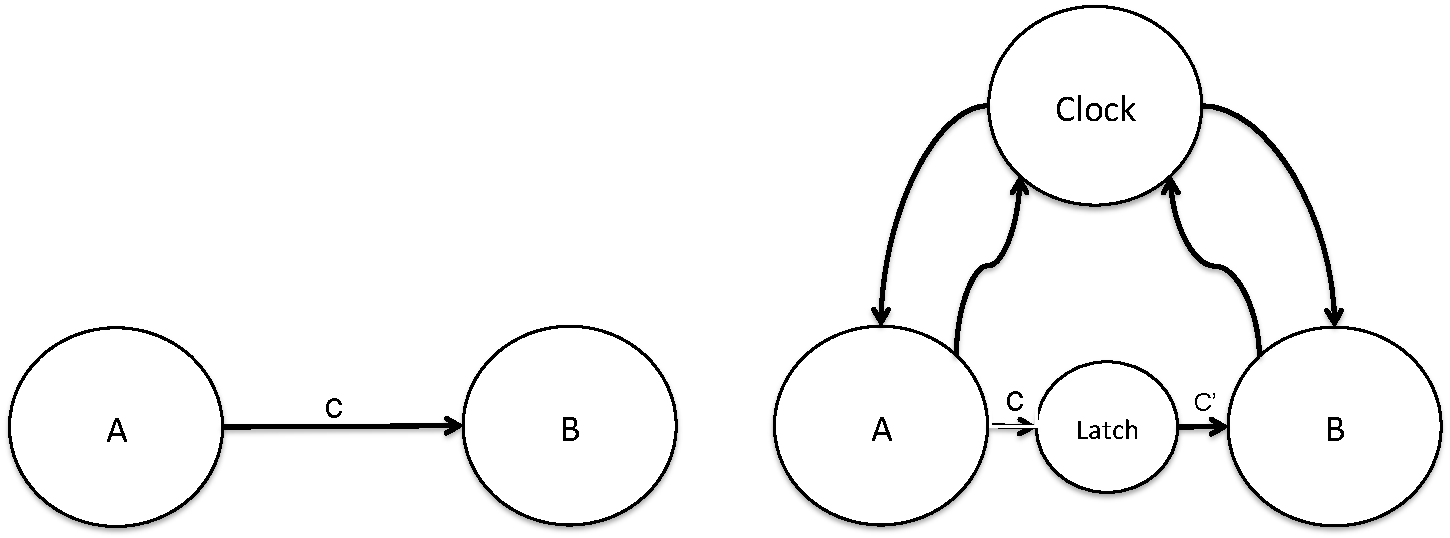
\includegraphics[width=10.0cm]{figures/clocked.pdf}
\caption{To enforce global synchrony on a simple reader-writer network in CSP, the complexity increase to include the clock and latch. Figure from \cite{Vinter2014}}
\label{fig:sme:clock_latch}
\end{figure}
\\\\
The advantage of using Python for this kind of processor simulation is the flexibility and simplicity of the language. It is easy to experiment with various ideas and versions but with the increased complexity of the added clock process and and clock-signal propagation, the advantages of Python seemed to diminish. Therefore the conclusion from the master thesis was that using PyCSP alone for building synchronous processor simulators was not feasible since the global clock was forced onto the CSP model. It was also concluded that external choice, which is a powerful and essential part of CSP, was not utilized in the globally synchronous approach. They did, however, conclude that several of other CSP concepts was fitting well with the hardware concepts, such as shared-nothing in CSP matches the structure of hardware communication.\\

After this attempt, it became clear that the structure of CSP was poorly suited for modeling clocked systems, and therefore it was decided to create the Synchronous Message Exchange framework, based on the CSP algebra. The idea was to only use the subset of the CSP algebra that provided beneficial functionality to hardware modeling which, most importantly, meant that external choice was omitted. However, the shared-nothing property of CSP showed to be very useful, since the network state could only be changed by process communication.
\\
% In SME the introduction of an implicit clock that eliminates the complexity caused by the model, described above, was imperative and is one of the key concepts hereof. The implicit clock removed the problems found by forcing the globally synchronous clock onto the CSP model. \\
In SME, a network is a combination of processes that are connected through buses. The processes communicate through a collection of signals in a bus, instead of CSP's synchronous rendezvous model, but retains the shared-nothing trait of CSP.
SME uses the term \texttt{bus} instead of \texttt{channel} to enforce the semantic correlation between the SME bus and a physical hardware signal bus.
The process communication is handled by a hidden clock which eliminates the complexity that arose from adding synchronicity to a CSP network. The combination of the hidden clock and the synchronous message passing between processes means that the SME model provides hardware-like signal propagation.

An SME clock cycle consists of three phases: it reads, executes, and writes as can be seen in Figure~\ref{fig:sme_process_flow}. The process is activated on the rising clock edge where it reads from the bus and it reads, executes and writes to the bus in one clock cycle. Just before the rising edge of the clock, all signals are propagated on all buses which means, that all communication happens simultaneously. Because of this structure, if a value is written by a process in cycle $i$, it is read by the receiving process in cycle $i+1$.

SME is able to detect read/write conflicts where multiple writes are performed to a single bus within the same clock cycle as well as reads from a signal that has not been written to in the previous clock-cycle.\\
All data, that are written to a bus can be logged for each clock cycle which means that these logs can be saved in a Comma-Separated Values, CSV, format and used for validating the VHDL implementation with a VHDL tool. This would eliminate the need to write seperate VHDL tests which will improve developer productivity immensely.

SME also supports clock-multipliers which means that a clocked network can have components inside the network being clocked at a different rate than its own clock. The rate can be an integer multiplier from its own clock. This means that all components are clocked relative to its parent network and therefore the clock will not need any extra coordination. It does however mean that the inner components can only fun faster than their parents.
% TODO: Do I really want this included?

Since an SME network is a network that can be represented as a graph, a diagram tool have also been implemented for SME. It utilizes the Graphviz tool to generate a visual graph of the network. This means that the SME networks can be generated and drawn as a graph which can help with debugging.
%TODO: Also, it this something I really want to include?


\begin{figure}[!ht]
  \centering
  \begin{tikzpicture}[auto]
    \node[mycircle, text width=2cm, shape=rectangle] (read) {Read};
    \node[mycircle, text width=2cm, shape=rectangle] (execute) [below=0.5cm of read] {Execute};
    \node[mycircle, text width=2cm, shape=rectangle] (write)  [below=0.5cm of execute] {Write};

    \draw [myarrow] (read) -- (execute);
    \draw [myarrow] (execute) -- (write);
    \draw [myarrow] (write) |-([shift={(5mm,-5mm)}]write.south east)-- ([shift={(5mm,5mm)}]read.north east)-| (read);
  \end{tikzpicture}
  \caption{SME process flow for one clock cycle.}
  \label{fig:sme_process_flow}
\end{figure}
Since SME is based on CSP, all SME models have a
corresponding CSP model, and because of this property, we are able to create a transpiler translating SME models to \cspm{}.
The SME model is currently implemented as libraries for the general-purpose languages C\#~\cite{Skovhede}, C++~\cite{asheim2015}, and Python~\cite{asheim2016vhdl}. The Python and C\# libraries both have code generators for VHDL as well.
\newpage
\subsection{SMEIL}
\label{SMEIL-section}
With the different SME implementations, a need arose for a common intermediate language. SME Implementation Language (SMEIL) was developed as a Domain Specific Language (DSL) for SME, usable both as an Intermediate Language, IL, and as an independent implementation language. It is accompanied with the implementation, \texttt{LIBSME}. %TODO: Find the reference in truls paper.
SMEIL has a C-like syntax with a specialized type system that makes hardware modeling simple. In spite of its simplicity, SMEIL still provides hardware-specific functionality that is more difficult to create with general-purpose languages.

Programs written in SMEIL are run by using the libsme library. This can be done either by using the command line utility or through the provided API.
The different methods of using SMEIL are:\\
\begin{itemize}
    \item \textbf{Pure SMEIL simulation:} A pure SMEIL program is a network which do not depend on outside influence. This means that the network  generates the data itself and the only communication are between the processes defined in the network.
    \item \textbf{Co-simulation of SMEIL:} The original intent with SMEIL was to create an intermediate language which could be used together with the general-purpose language implementations of SME, which is called co-simulation. With co-simulation, a test bench can be generated as well as VHDL code.
    \item \textbf{Direct code generation:} A SMEIL program which does not need to simulate before generating VHDL. In this case all types are constrained and all information needed for the code generation are in place. Because the simulation step is not executed, a VHDL test bench is also not automatically generated, since this happens in the simulation step.
\end{itemize}
The base entity of an SMEIL program is the module which corresponds to a file. The module consists of the actual SMEIL program as well as import statements. SMEIL programs can be seperated into modules which can then be importet into other SMEIL programs, creating a library-like structure and reusable components.\\

The SME model supports both synchronous and asynchronous processes. A synchronous process are run during every clock-cycle and an asynchronous process are only run when receiving a signal on the input bus, but unfortunately SMEIL does not currently support asynchronous processes. %TODO: Ask truls if it is implemented in other sme implementations.
\\

The two fundamental components of an SMEIL program is \texttt{process} and \texttt{network}. The process consists of variable and bus definitions, as well as the statements that are evaluated once for each clock cycle. The purpose of the \texttt{network} declaration is to define the relations between each entity in the program. A small example of process and network syntax can be seen in Listing~\ref{lst:smeil_small_syntax_example} and a further introduction to the language can be found in Section \ref{chap:analysis}.\\
\begin{listing}
\begin{minted}[escapeinside=||, mathescape=true]{smeil_lexer.py:SMEILLexer -x}
proc addone (in inbus)
    bus outbus {
        val: int;
    };
{
    outbus.val = inbus.val + 1;
}

    |$\vdots$|

network net() {
    instance a of addone(b.outbus);
    instance b of ..
    |$\vdots$|
}
\end{minted}
\caption{Small example of process and network syntax in SMEIL.}
\label{lst:smeil_small_syntax_example}
\end{listing}

\subsubsection{SMEIL type system}
The SMEIL language is stongly, statically typed and has a simple type system that is checked at compile-time. The purpose of SMEIL is to be able to model hardware, and since hardware is static, it was important to create a type system that was cabable of enforcing as many static invariants as possible. Therefore only between signed and unsigned integers is type coercion performed in SMEIL, which also means that only booleans can be used in conditionals.
It is easy to transform a statically typed language to a dynamically typed language, but not the other way around, therefore SMEIL will be simple to translate to various different target languages.

The SMEIL type system differs from standard general-purpose languages mainly on the support for bit-precise types. In general-purpose languages it is typical targeted a CPU which consists of fixed-width registers which typically means that it can not work with data smaller than a byte. This is, however, an important part of modeling hardware to be able to define the exact widths of the wires in order to optimise the hardware implementation. SMEIL supports unlimited-size integers as well as integers constained to a specific bit-length. SMEIL also supports booleans, double and single precision floating point numbers as well as strings. Currenly, floating-point numbers are not supported in the SMEIL hardware-translations. %TODO Venter på svar omkring hvad det her egentligt betyder? Og tjek lige at jeg ikke også skriver om det i analyse.
Arrays of a fixed length of the types, mentioned above, are also supported.

In SMEIL buses are represented as channel names and their types, and since processes or networks can accept buses passed as parameters it is important to ensure that no process or network is instantiated with a bus that does not contain the expected channels.
In the same way, it is essential to ensure that the directionality of the bus is enforced. When buses are passed as parameters, they are explicitly declared as either input or output bus. However, when defining a bus within a process it is not possible to define the directionality of the bus. Therefore the bus are defined as input or output based on their first use.
The type system of SMEIL is enforcing a set of rules that define how two buses are unified and the directionality of the bus, which ensures that problems such as the ones described above, does not happen.
All types of declarations in SMEIL are private exept bus declarations. As mentioned above, they are used for establishing communication between processes and therefore needs to be a part of the public interface of a process or network.

\subsubsection{Simulating SMEIL programs}
When translating SMEIL to hardware models, it is necessary to have all types in the program constrained to a specific width. However, as mentioned before, SMEIL does support unlimited size integers. Since it can be difficult to define an optimal width when writing the SME model, there was a need to provide both the support of the unlimited size integers while still being able to translate to hardware descriptions.
Therefore libsme provides a way to re-type the SME network based on the values that where observed during the simulation of the program.
During the simulation, the observed minimun and maximum value for all variables and channel are captured and saved along with the original value.
After the simulation, these minimum and maximum values are then converted into SMEIL types large enough to hold the range.
The new SMEIL program with the updated types and observed ranges are then passed through the type checker, in order to ensure that all constraints from the original program is still respected.
% An example of this can be seen in Figure \ref{fig:smeil_restricted_types_and_ranges} where a unlimited size integer is re-typed to an integer of fixed size after the simulation. In Figure \ref{fig:invalid} an example of a violation can be seen. Here the value c is contrained to \texttt{i10} but if the channel \texttt{b.chan} observe values that are 16-bit long then the restrictions on the c variable are violated.

% \begin{figure}
%   \centering
%   \begin{subfigure}[t]{0.25\linewidth}
%       \begin{listing}
%       \begin{minted}[escapeinside=||, mathescape=true]{smeil_lexer.py:SMEILLexer -x}
%           proc A ()
%            bus b {
%             chan: ?{\bfseries\underline{int}}?;
%            };
%            var c: i10;
%           {
%            c = b.chan;
%           }
%       \end{minted}
%       \end{listing}
%     \caption{Unconstrained types.}
%     \label{fig:oktype}
%   \end{subfigure}
%   \begin{subfigure}[t]{0.35\linewidth}
%   \begin{listing}
%   \begin{minted}[escapeinside=||, mathescape=true]{smeil_lexer.py:SMEILLexer -x}
%       proc A ()
%           bus b {
%               chan: ?{\bfseries\underline{i6 range 0 to 29}}?;
%           };
%           var c: i10;
%       {
%        c = b.chan;
%       }
%   \end{minted}
%   \end{listing}
%     \caption{Valid.}
%     \label{fig:non-violated}
%   \end{subfigure}
%   \begin{subfigure}[t]{0.35\linewidth}
%   \begin{listing}
%   \begin{minted}[escapeinside=||, mathescape=true]{smeil_lexer.py:SMEILLexer -x}
% proc A ()
% bus b {
% chan: ?{\bfseries\underline{i16 range 0 to 30717}}?;
% };
% var c: i10;
% {
% c = b.chan;
% }
%   \end{minted}
%   \end{listing}
%     \caption{Invalid.}
%     \label{fig:violated}
%   \end{subfigure}
%   \caption{Shows a process entering the simulator with an unconstrained type (a)
%     and examples of two possible resulting programs (b, c). The type changing
%     between the examples is underlined.}
%   \label{fig:simtyping}
% \end{figure}
% NOTE: THis figure does not compile. It is taken from Truls article and I should change the captions and also mention where I got it from.

% In Figure \ref{fig:smeil_restricted_types_and_ranges} the two last programs, showed in Figure x and y, will be the result of the re-typing of the program after simulation. That is, the programs resulting from the simulation of the program in Figure z.


\subsubsection{Co-simulation}
Often when modeling hardware in Hardware Description Languages (HDLs) like VHDL or Verilog, code for testing and verifying are often written in the same language as the design itself. Unfortunately, the HDLs often does not have the functionality for generating proper simulation input. Using general-purpose languages for testing hardware models are useful since the range of available libraries are much larger.
Therefore the SMEIL simulator provides a simple language-independent API which enables SME implementations written for general-purpose languages to communicate with SME networks written in SMEIL, so-called co-simulation.
The big advantage of the SMEIL approach to co-simulation is that SME is used on both sides of the co-simulation and therefore both sides acts as a single entity.
The PySME %TODO: Reference
library have been extended to support co-simulation with SMEIL, thereby providing the posibility of writing networks in PySME which can interact with SME networks written in SMEIL. Currently, this extension have only been implemented in the PySME implementation, but is expected to be implemented in the other SME implementations as well.\\
Another functionality of the libsme compiler is, when simulating the SMEIL network, the compiler can record a trace of all communication between processes in the network. This trace file can then be used as a source for the VHDL test bench which can be used to verify the generated VHDL code.

% Some parts of the SMEIL grammar is not implemented in SMEIL yet and therefore we are also not supporting these.
In Figure~\ref{fig:smeil_transpiler} the SMEIL transpiler structure can be seen.

\begin{figure}[!ht]
  \centering
  \begin{tikzpicture}[auto]
    \node[mycircle, minimum size=1.75cm, align=center, text width=1.75cm, font=\footnotesize]    (smeil)                                       {SMEIL};
    \node[myrectangle, text width=1.5cm, minimum height=1.0cm, inner sep=5pt, inner ysep=5pt] (csme)  [above left=-0.25cm and 1.5cm of smeil] {C\#SME};
    \node[myrectangle, text width=1.5cm, minimum height=1.0cm, inner sep=5pt, inner ysep=5pt] (pysme) [below left=-0.25cm and 1.5cm of smeil] {PySME};
    \node[myrectangle, text width=1.5cm, minimum height=1.0cm, inner sep=5pt, inner ysep=5pt] (vhdl)  [right=1.0cm of smeil]                {VHDL};

    \draw[myarrow] (csme)  -- (smeil);
    \draw[myarrow] (pysme) -- (smeil);
    \draw[myarrow] (smeil) -- (vhdl);
  \end{tikzpicture}
  \caption{SMEIL transpiler structure.}
  \label{fig:smeil_transpiler}
\end{figure}




\newpage
\section{CSP}

Today, Communicating Sequential Processes (CSP) \todo{reference} is a process algebra that provides a way to express concurrent systems. By using message passing between processes the language avoids certain problems that arise with the use of e.g shared variables. An essential part of CSP is message passing and the syntax for input is \texttt{X?c}. This represents an input from channel\texttt{X} and an assignment of the input value to the variable \texttt{c}. The output syntax is \texttt{X!c} where the value of the variable \texttt{c} is sent over the output channel \texttt{X}. At first Hoare had defined the message syntax to use the process names, but later on when CSP was developed into a proper process algebra, the syntax changed into using channels in order to be able to have several processes connected via the same channels. % TODO: do not write too much here. just short explain csp

\subsection{\cspm{}}
%CSPm was devised by Bryan Scattergood as a machine-readable dialect of CSP  - se the paper \textit{The Semantics and Implementation of Machine-Readable CSP}\\\\
\cspm{} is a formal language that combines CSP with a functional programming language in order to make it easier for the programmer to model the systems and then use the code on tools that can animate, verify or similar.


\subsection{FDR4}
%" FDR2 is often described as a model checker, but is technically a refinement checker, in that it converts two CSP process expressions into Labelled Transition Systems (LTSs), and then determines whether one of the processes is a refinement of the other within some specified semantic model (traces, failures, or failures/divergence)" (from Wikipedia - se paper \textit{Model-checking CSP - af Roscoe} \\\\
FDR (Failures Divergence Refinement) tool is a refinement checker for

In the paper \textit{A primer on model checking}\cite{Ben-ari2010} Mordechai Ben-Ari explains a concurrent problem that he had used for many years, to teach his students about concurrency. ... % TODO: write this when I have read the article again


We not only want to transpile SMEIL to \cspm{}, we also want to be able to verify different properties in \cspm{} in order to prove correctness. Today, there exists several tools for formal verification, both in academia and in the industry. One of the currently most favored tools is the Failures-Divergences Refinement tool (FDR4). This tool is a CSP refinement checker that can analyze programs written in the machine-readable version of CSP; \cspm{}.
It provides a parallel refinement-checking engine that can scale up linearly with the number of cores. This means that it can handle processes with a large number of states in a reasonable time. FDR4 can handle several different types of assertions, deadlocks being the most used. However, due to the structure of SMEIL, we use FDR4 in a different way than is typical. Since the SME model cannot have cyclic-wait we have no need to verify the system in this manner.

For our current implementation of the transpiler, we can assert the ranges of the channel inputs, for example, we can automatically assert that the observed ranges, provided by the SMEIL simulation, and the possible input on the \cspm{} channels are not conflicting.
In hardware, we would typically want to verify that the communication on a bus does not exceed a certain range or that the sum of multiple signals does not exceed a specific value. A bus might be able to carry other data than needed, and being able to model a circuit that can assert that the bus never carries other data than expected, is of great value.
\\

CSP was not initially developed for hardware modeling, and therefore it is not evident how to handle the clock cycle, which is an essential part of hardware modeling. When we transpile the SME network into \cspm{} the SMEIL simulation have provided the ranges of all values from the simulation and therefore all clock cycles. This means that when FDR4 asserts a property it asserts on all possible communication combinations for all the simulated clock cycles. Therefore, even though we are transpiling from an SME model, where the clock is crucial, we can simply translate ``one-to-one" from the SMEIL program and still get an accurate assertion on the properties.


%
% \chapter{Analysis}
% \label{chap:analysis}
% %!TEX root = ../main.tex

% This section should contain information about the problem, but not the solution. I am analysing the problem and explaining what will be problematic when translating from SMEIL to CSPm.

% Der er tre dele i SMEIL jeg har interesse i:
% Three components: Behavioral, structural, meta data

% Jeg skal ikke fortælle hvordan jeg har gjort det men analyse af problemet og ikke af løsningen. Jeg skal blot beskrive problemstillingerne.
In this section we analyse the differences between the SMEIL model and the functionality of \cspm. We also introduce important parts of the SMEIL structure and grammar to provide an understanding of the different challenges.

\section{Verification}
\label{sec:analysis_verification}
% TODO: Still not sure I introduce the problem properly
The reason for translating SMEIL to \cspm{} is to use the refinement checking property of the CSP language. By loading the \cspm{} programs into FDR4 we can verify different properties within the SMEIL program.
Before we can design the transpiler and generate the \cspm{} code, it is essential to figure out what kind of properties would be beneficial to verify in hardware, and what kind of properties are possible to verify with FDR4.
As mentioned in Chapter \ref{chap:background}, FDR4 provides refinement checking with different models. FDR4 is often used for deadlock checking, but since the SME model guarantee deadlock freedom, it will not be necessary to use this property within FDR4\footnote{It might be interesting to do the deadlock checking simply to verify that the translation was done correctly. The generated \cspm{} code should also be deadlock free}.\\

In hardware, we would typically want to verify that the communication on a bus does not exceed a certain range or that the sum of multiple signals does not exceed a specific value. A bus might be able to carry other data than needed, and being able to model a circuit that can assert that the bus never carries other data than expected, is of great value.

Therefore it would be interesting to verify that certain values are never communicated on a specific channel, or that they are the only values communicated on the channel.
When designing hardware it is always designed as a single unit but typically it will be connected with other units, creating a bigger structure. It is difficult to know exactly what input the network will have to handle and therefore it is interesting to be able to assert exactly what values can be communicated on the channels but also how the network react when unforseen values are input.

To provide an understanding of the problem this kind of verification would be able to solve, we here introduce an example that will be referred to several times throughout the thesis.

\subsection{Seven Segment example}
\label{sec:example-seven_segment_intro}
A seven segment display is an electronic display device which is used in displays such as digital clocks or other types of devices that display numerals. An example of a typical digital clock display can be seen in Figure~\ref{fig:6_displays}. As the name states, each display consists of seven segments which can be lit up in patterns to display symbols, like numerals.
When a digit has been determined for a seven segment display, it is encoded to a bitstream that represents the digit in the correctly activated display segments.
\begin{figure}[!ht]
  \begin{center}
    \tikz{
      \node[inner sep=5pt, outer sep=2pt, draw=blue] {
        \sevensegnum[size=2em, shrink=0.1]{1}
        \sevensegnum[size=2em, shrink=0.1]{2}
      }
    }
    \tikz{
      \node[inner sep=5pt, outer sep=2pt, draw=blue] {
        \sevensegnum[size=2em, shrink=0.1]{3}
        \sevensegnum[size=2em, shrink=0.1]{4}
      }
    }
    \tikz{
      \node[inner sep=5pt, outer sep=2pt, draw=blue] {
        \sevensegnum[size=2em, shrink=0.1]{5}
        \sevensegnum[size=2em, shrink=0.1]{6}
      }
    }
  \end{center}
  \caption{Digital clock with six seven segment displays, displaying 12:34:56.}
  \label{fig:6_displays}
\end{figure}
In this example, we wish to model a typical digital clock that is able to calculate and display the current time in hours, minutes, and seconds. Listing~\ref{lst:python} shows this example written in Python.

Like \texttt{time\_since\_midnight} in Listing~\ref{lst:python}, the network must have some input of data. The input value represents seconds since midnight, and in order to calculate hours, minutes, and seconds we model three different processes, called the \texttt{time} processes in this example.

When writing hardware models in pure SMEIL, the only way to generate input for the network is to create a data generator process. This process, called the \texttt{clock} process in our example, is instantiated with a start time and is incremented by 1 for each simulation cycle, representing a one second increase.
% TODO: Do I need to move this further down? It might be that SMEIL have not been introduced properly so they wont understand it yet. It is an option to move it after Meta..
The result is communicated on the process output bus, where the three \texttt{time} processes are listening. These \texttt{time} processes receive the number and by the use of simple integer arithmetic, calculate the hours, minutes, and seconds since midnight respectively. It is obvious that at some point in time, each \texttt{time} process will calculate a two-digit result, for example at 12 hours or 42 seconds. However, a single seven segment display can only show one digit between 0 and 9. Therefore we need two seven segment displays for each \texttt{time} process in order to show the correct time in a 24-hour interval. Each \texttt{time} process has an output bus with two individual channels that represent the communication to each different display. The number representing either hours, minutes, or seconds are separated into first and second digit, by $\lfloor \frac{x}{10} \rfloor$ and $(x \text{ mod } 10)$. These six different results are then communicated onto the six different channels which represent the six different seven segment displays.
The outline of this network can be seen in Figure~\ref{fig:smeil_network}.\\
\begin{listing}
\begin{minted}[escapeinside=||, mathescape=true]{python}
from math import floor

def time(time_since_midnight):
    hours   = floor(time_since_midnight / 3600)
    minutes = floor((time_since_midnight - hours * 3600) / 60)
    seconds = time_since_midnight - hours * 3600 - minutes * 60
    return [hours, minutes, seconds]

print(time( 57100)) # =>  15:51:40
print(time(  3601)) # =>  01:00:01
print(time( 66666)) # =>  18:31:06
\end{minted}
\caption{A Python implementation of the seven segment display example.}
\label{lst:python}
\end{listing}
\begin{figure}[!ht]
  \centering
  \begin{tikzpicture}
    \node [mycircle] (I) at (0,0) {$I$};

    \node [mycircle] (H) at (2.5,  1.50) {$H$};
    \node [mycircle] (M) at (2.5,  0.00) {$M$};
    \node [mycircle] (S) at (2.5, -1.50) {$S$};

    \draw [myarrow] (I) -- (M);

    \draw [myarrow, smooth] (I) to[out=0, in=180] (H);
    \draw [myarrow, smooth] (I) to[out=0, in=180] (S);

    % Output arrows without processes
    \draw [myarrow] (3.125,  1.625) -- (4.000,  1.750);
    \draw [myarrow] (3.125,  1.375) -- (4.000,  1.250);
    \draw [myarrow] (3.125,  0.125) -- (4.000,  0.250);
    \draw [myarrow] (3.125, -0.125) -- (4.000, -0.250);
    \draw [myarrow] (3.125, -1.375) -- (4.000, -1.250);
    \draw [myarrow] (3.125, -1.625) -- (4.000, -1.750);
  \end{tikzpicture}
  \caption{SMEIL network for a seven segment display clock. Each SMEIL process is represented by a cicle with a letter corresponding to the processes Input, Hours, Minutes and Seconds respectively.}
  \label{fig:smeil_network}
\end{figure}

In Figure~\ref{fig:smeil_network} the network consists of four processes, the data generator process, \textit{I}, which creates the input that is broadcasted out on the network. The three \texttt{time} processes, hours (\textit{H}), minutes (\textit{M}), and seconds (\textit{S}) are the processes described above, which calculate each part of the current time. The outputs are communicated on the six outgoing channels.\\

In this example the properties we wish to assert with FDR4, are the width of the channels. That is, we want to prove that certain values will never be communicated on certain channels.
One could imagine that 4 bits can be communicated between the \texttt{time} processes and the seven segment displays. But 4 bits can represent the numbers 0 through 15, and our seven segment displays can only display the numbers 0 through 9. Therefore we wish to assert that even though the channels can carry 4 bits, the actual communication on the six output channels does not exceed 9. In general, the displays will be able to display 0 through 9, but since the example is a clock showing a 24-hour interval, the displays will of course not be able to show minutes and seconds above 59 and hours above 23.

The full SMEIL code for this example can be seen in Listing~\ref{lst:smeil} in  the appendix.

\section{Transpiling SMEIL to \cspm{}}
\label{sec:transpiling}
Since we are translating code from SMEIL to \cspm{}, the challenge it to find \cspm{} structures that corresponds to the SMEIL strucutres. The ultimate goal is to find methods for transpiling, that can be generalised to most problems.

From the introduction to both SMEIL and \cspm it is clear that the main intention of each language is different and therefore the transpiling of a process in SMEIL to a \cspm process might not be completely trivial.
% All data from the SMEIL process will need to be translated into data and structures within the \cspm model, calculations and communications alike.

% TODO: Something about functional language to imperative language


% Vigtigt at have de tre dele adskilt i afsnittet. Brug figuren fra side 107 i bujo til at henvise til at jeg har en Magic 8-ball (Mit system) og jeg skal fra SMEIL til FDR og henvise til at det er det flow jeg har brug for.


% I SMEIL har jeg et prædefineret konsistent navnerum. Jeg skal ikke lave en symboltabel. Jeg arver direkte fra SMEIL til CSPm. Så her kan jeg snakke om at hvis jeg gjorde det på en anden måde ville jeg ikke kunne gøre det sådan. Det skal jeg skrive om her. TODO: Make a decision about where this belongs. It does not seem to be fitting in with the analysis, but on the other hand this was what Brian told me. But is he right?


When analysing the general structure of SMEIL programs, there are three structures that are particular interesting when we are interested in translating from SMEIL to \cspm{}. These three structures are:
\begin{enumerate}
    \item \textbf{Behavioral:} The general behavior of each process and function.
    \item \textbf{Structural:} How the circuit is connected, i.e which buses connects to which processes.
    \item \textbf{Meta information/Observed values} %TODO: Meta information or observed values?:
    All data information from the SMEIL network that could be beneficial for our translation to \cspm{}.
\end{enumerate}

% TODO: Should I add the clock problem to the list, so it becomes four parts?

\subsection{Behavioral}
%% - Behavioral description - hvad den enkelte funktion gør. det oversættes ret nemt. Jeg bekymre mig ikke om variable og sådan nogle ting. Det er allerede gjort før det gøres til SMEIL, og dem kan jeg genbruge i min code generation.  Funktionel indhold af processer/ opførsel af den enkelte process - det er rimelig nemt oversat direkte til CSPm. Her kan man beskrive hvis der er nogle sproglige udfordringer, fx hvis CSPm ikke har loops eller lign.
The behaviour of the single process in the SMEIL program is the base of the functionality of the SMEIL program. By analysing the different structures of processes in SMEIL, we can get a sense of how it should be created in \cspm.
\subsubsection{Processes}
% TODO: Maybe I only need to introduce SMEIL stuff that TAPS support?

% %%%% SMEIL processes %%%%
An SMEIL process is defined by the \texttt{proc} keyword and consists of an identifier, process parameters, bus and variable declarations. The body of the process, or the process statements, consists of sequential statements such as communications and calculations that are to be evaluated once for each clock cycle. A small example of a SMEIL process can be seen below. The process \texttt{A} takes an input bus, \texttt{i}, and writes on its own output bus \texttt{a\_bus}.
\begin{minted}[linenos=false, escapeinside=||, mathescape=true]{smeil_lexer.py:SMEILLexer -x}
proc A (in i)
    bus a_bus {chan : int}
    {
        a_bus.chan = i.chan + 1
    }
\end{minted}

It is not possible to declare variables inside the process statements and therefore all variable and communications must be declared in the declarative part of the process. This attribute should simplify the translation to \cspm, since TAPS will only have to search the declarative part of the process to find all variable and bus definitions.
A process can be instantiated with a set of parameters. These parameters can be a mix of input and output buses and constants. A process is initiated in the network of a SMEIL program which will be explained later.\\

In the SMEIL grammar, it is possible to declare if the process is \texttt{sync} or \texttt{async}. A \texttt{sync} process is run during each clock cycle, and a \texttt{async} process is only run when they receive a signal on the input bus. The current implementation of SMEIL does not support \texttt{async} processes, which means that all SMEIL process are in sync and behaves like decribed in Chapter \ref{chap:background}, where they read and write once in each clock cycle.
The syncronicity of the processes are an essential part of the SMEIL network and therefore it is crucial that the generated code is able to model this correctly. In \cspm{} a process does not communicate until it receives an input, which match the async process of SMEIL. However, since it is only the  synchronous processes that are supported in SMEIL, it is necessary to introduce
a structure to the \cspm network, that simulates the synchronous structure of the SMEIL proceses.
\\

In an SMEIL process, the declarative part of the process can consists of different variables and constants as well as bus definitions. In this next part we introduce variables and constants, whereas buses are described in section \ref{sec:analysis_structural}.
\paragraph{Constants}
Constants are used when declaring named constant values and consists of an identifier, a type and an optional expression. The expression could be simply an integer assigned to the constant, for instance:
\begin{minted}[linenos=false, escapeinside=||, mathescape=true]{smeil_lexer.py:SMEILLexer -x}
const hours: uint = 24;
\end{minted}
Variables are very similar to constants but simply hold mutable values within the process. In SMEIL variables persist their values in between clock cycles, which mean that it is possible for a process to save a value or result and reuse it in the next clock cycle.
\paragraph{Variables}
The only difference between variable and constants in SMEIL, is that variables can also take a range of values, for example:
\begin{minted}[linenos=false, escapeinside=||, mathescape=true]{smeil_lexer.py:SMEILLexer -x}
var minutes: u6 = 0 range 0 to 59;
\end{minted}
The assignment of \texttt{= 0} is simply to give an initial value of the variable, but is optional, as well as the ranges are optional. The range give an expected value range of the variable. When simulating the SMEIL program, the range of observed values are used to define the type of the variable.

In SMEIL, the types of variable and constants must always be defined and this also applies to bus channel declaration. The types can be either unlimited size integers, \texttt{int} and \texttt{uint}, or restricted to a specific bit-length. The prefixes \texttt{i} and \texttt{u} refers to signed and unsigned integers followed by a number determining the bit-length. For instance, \texttt{i4} represents a signed 4-bit integer.
The unlimited bit size \texttt{int} and \texttt{uint} are not realistic to have in \cspm since, when verifying a program, FDR4 will look at the entire possible statespace, and with unlimited integers the statespace will be enormous. FDR4 restricts its integer types to signed 32-bit\cite{UniversityofOxford}. \cspm does not apply types to its variables and constants the same way as SMEIL and \cspm also does not support all the types that SMEIL support.
Because of the type-system of SMEIL the libsme compiler will provide a warning if the values or ranges assigned to a constant or variable are above or below what the type can represent. In the example below the number 59 cannot be represented by 4 bits and therefore it would cause a warning from the compiler.
\begin{minted}[linenos=false, escapeinside=||, mathescape=true]{smeil_lexer.py:SMEILLexer -x}
var minutes: u4 = 0 range 0 to 59;
\end{minted}

In the SME model, processes never terminate, but when simulating an SMEIL program, it is necessary to terminate the simulation at some point, but it should simply be seen as a snapshot of the process and not that the process terminates when the simulation ends.
The number of clock cycles, the simulation is run for, is specified via the command line tool.
There is, of course, limitations to the simulation, and it is important to note that the simulation is a simple tool to simulate the running system, however it does necessary provide all possible results of the system. If a system fails at a 1000 clock cycles, but the system is only simulated for 100 clock cycles, then we would not know about the failure. If the translation use the observed values from a simulation, the user need to know the limitations of the simulation.
% If the simulation is not passing through enough clock cycles, the verification might be inadequate. Since the verification builds on the observed values, the simulation needs to be long enough such that the whole possible range of input values is exhausted. %TODO: Where should I add this? Removed it from the background section

In \cspm, constant can be declared as we know it from many other languages;
\begin{minted}[linenos=false, escapeinside=||, mathescape=true]{cspm_lexer.py:CSPmLexer -x}
N = 5
\end{minted}
and variables can be used without declaring them first, for example in a process declaration with a local definition.
\begin{minted}[linenos=false, escapeinside=||, mathescape=true]{cspm_lexer.py:CSPmLexer -x}
Proc(x) =
    let
        m = x % 60
    within
        channel ! m -> SKIP
\end{minted}
A variable is also defined when communication specific values over channels in \cspm. For example in the example below, the received value is assigned to the variable $x$ which is then used when writing the value out in the \texttt{output} channel.
\begin{minted}[linenos=false, escapeinside=||, mathescape=true]{cspm_lexer.py:CSPmLexer -x}
P = input ? x -> output ! x -> STOP
\end{minted}

Translating constants and variables from SMEIL to \cspm will not prove difficult, since the structures are quite similar.
A potential challenge lies in deciding how to define a variable that has been declared with initial value in SMEIL, since this mean that the \cspm translation will have to define the variable before it is used within the calculations.\\
% \paragraph{Enumerations}
% In SMEIL it is also possible to declare enumerations within a process or a network declaration. Emumerations can be used to referencing symbolic constants instead of its numerical constants which can improve the readability of the program.
% Currently enumerations are not implemented in TAPS.
% TODO: Enummerations are not implemented in TAPS, so should I even write about it here?


% TODO: Should I say something about Generators?
% \paragraph{Generators}
% SMEIL does not support this, so I also wont support this and therefore I might not need this paragraph. It is however interesting because it is kind of a foor loop, but not because of the side effects but to simplyfy generation of code structures.


The other part of an SMEIL process is the statement part where the actual behaviour of the process is defined. The semantics of statements in SMEIL corresponds to what we typically see in C-like languages.
\paragraph{Assignments}
An assignment in SMEIL consists of a name and an expression. It can be used in two different ways within the SMEIL process statements: assigning to a variable and assigning to a bus channel. In SMEIL the compiler will always be able to recognise what is being assigned by looking at the type of the object and therefore SMEIL do not differentiate between these two assignments.
This property will cause a challenge when translating to \cspm{}, since communication and variable assignments are two different things in a \cspm program. Thus TAPS will have to be able to recognise what type of assignment it is, in order to create the correct translation.
\paragraph{if-statements}
If-statements are structured like we know from other languages with an if-expression, then-expression, elif-expression and an else-expression.
These kinds of statements can also be defined in \cspm, but \cspm does not support elif-expressions within the if-statement, so the translation would have to restructure the elif-expression to a nested if-expression.
Since the structure of the \cspm process is different, an if-statement might have a different context in the \cspm program. It is possible that TAPS have to take extra precautions to provide the correct context to the if-statement.
% \paragraph{Loops}
% TODO: Write something here when I am sure how loops work in CSPm.

\paragraph{Traces and assertions}
The trace statement in SMEIL is not affecting the behaviour of the process, but it simply prints out the string and arguments that is given, like a printf in C.
In \cspm it is possible to add a print statement, but this will appear in the right hand side of the FDR4 session window for easy evaluation, and it does not support printing out text, but rather calculations. Thus the trace statements in SMEIL is not compatible with \cspm and either the trace statements should be thrown away or kept as a comment in the generated code.\\

The assert statements are used internally in SMEIL and evaluated during program execution. If the assert statement is not valid, then the execution is halted and the error message, defined in the assert statement, is printed, for instance
\begin{minted}[linenos=false, escapeinside=||, mathescape=true]{smeil_lexer.py:SMEILLexer -x}
assert(hour < 23, "hours cannot be greater than 23");
\end{minted}

Even though we wish to assert properties in FDR4, the properties that FDR4 can verify are not similar to the properties that the assert statements in SMEIL are asserting. As was introduced in Section \ref{sec:background_fdr}, FDR4 is a refinement checker and the assert statements in FDR4 are asserting the refinement check. In the \cspm language, assertions like \texttt{assert 4 + 4 == 8} is possible, however FDR4 does not support this. The two types of assert statement are therefore not equivalent. However, it should also not be of interest to translate the SMEIL assert statements, since a potential error found via an SMEIL assertion, might as well be found and corrected in SMEIL than in FDR4.
% \paragraph{Switch statements}
% TODO: Write something about switch statements when I know more.

\paragraph{Expressions}
Expressions in SMEIL and their precedence rules are similar to C-like languages and we will therefore not introduce them further. Expressions are used for defining operations and naming in SMEIL.

In \cspm the standard binary operators like \texttt{+}, \texttt{-}, \texttt{*}, \texttt{/}, and \texttt{\%} all take two arguments of type \texttt{Int} and return a value of type \texttt{Int}. It is important to notice that in \cspm, the \texttt{/} operator returns the quotient and rounds towards negative infinity. The \texttt{\%} operator in \cspm returns the modulus.
Floating point number are, not supported by FDR4\cite{Scattergood2011} which is also clear from the fact that the binary operators take only \texttt{Int} as their inputs.
As mentioned in Section \ref{sec:background_smeil}, SMEIL supports floating poitn numbers in the simulator, but it has not been extensively tested.

The unary \texttt{-} operator, representing a negation of an integer and the unary \texttt{!} operator, representing logical negation are both represented in the FDR4 syntax. The relational operators \texttt{<}, \texttt{>}, \texttt{<=}, \texttt{>=}, \texttt{==} and \texttt{!=} returns boolean values both in SMEIL and in \cspm. The logical conjunction and disjunction operators \texttt{\&\&} and \texttt{||} are also represented in both SMEIL and \cspm and both only accepting boolean values.
The presedence of the above mentioned operators are not entirely identical across SMEIL and \cspm, so it might be necessary to add extra parentheses to keep the correct semantic.

% SMEIL also supports shift operations which is not supported in FDR4, but...
% The programming languages C, C++, and Go, however, have only one right shift operator, >>. Most C and C++ implementations, and Go, choose which right shift to perform depending on the type of integer being shifted: signed integers are shifted using the arithmetic shift, and unsigned integers are shifted using the logical shift. - From wiki
% TODO: Ask truls about what kind of shift it is
% TODO: Find out how many of the operators are actually possible to use in CSPm.
% \texttt{<<}, \texttt{>>}, \texttt{&}, \texttt{|}, \texttt{^}, \texttt{+}(identity), \texttt{~}(bitwise not),

% TODO: Write something about array types. Can we have that in CSPm?(Page 25 in truls master)

% %%%% CSPm processes %%%%
As mentioned above, processes in SMEIL can be defined with parameters which represents input and output buses as well as constants. In \cspm{} processes can also be defined with parameters that can be variables, channels or similar.
In \cspm the processs behaviour also represents functionality, but the behaviour is often more focused on communicative behaviour between other processes. A typical process in \cspm could look like the one in Listing \ref{dining_philosopher_cspm} which represents a philosopher process from the dining philosophers problem. The process behaviour shows a philosophers actions in communicating with other processes. As can be seen, the process also conduct some simple calculations, but the main structure consists of communication, which is the purpose of \cspm, to be able to verify communication between parallel processes.
\begin{listing}
\begin{minted}[escapeinside=||, mathescape=true]{cspm_lexer.py:CSPmLexer -x}
PHIL(i) = thinks.i -> sits!i -> picks!i!i -> picks!i!((i+1)%N) ->
          eats!i -> putsdown!i!((i+1)%N) -> putsdown!i!i -> getsup!i -> PHIL(i)

\end{minted}
\caption{A dining philosopher process from the dining philosophers problem example file provided at the FDR4 webpage~\cite{fdr_example}.}
\label{dining_philosopher_cspm}
\end{listing}

The translation of processes from SMEIL to \cspm does include challenges and cannot be translated directly. In SMEIL the calculations of the process is as important as the communication whereas in \cspm it is often the other way round. The challenge lies in structuring the \cspm process in a way that gives the same functionality while still keep the \cspm communication behaviour and the assertion properties.

\subsubsection{Generating data}
%%%%% Generator processes %%%%%
When writing pure SMEIL programs, there will always be a need to generate input for the network. If the program was not written as pure SMEIL, the input for the network would be provided by the surrounding code. But in the case of pure SMEIL, the input data must be generated, which can be done in a few ways.
One way of initialising the network is by instantiating the processes with constants given as a parameter or hard code internal values into the process. These values will then act as the starting point of the network. Another way of initialising data in the SMEIL network, is to have a seperate process creating data for the network. We call this a data generator process.

An example of a process being instantiated with a constant can be seen in Listing \ref{lst:addone_data_generation_example}. Here we see the \texttt{Addone} network, which is a simple SMEIL network with two processes. The \texttt{add} process receives an input value, add the constant value to the input and writes it out on the outbus bus. The \texttt{id} process receives an input and writes it to its output bus imediately. Networks in SMEIL are introduced further in Section \ref{sec:analysis_structural}, but the network in this example is simply defining the input bus of the \texttt{add} process to be the output bus of the \texttt{id} process, as well as defining that the constant value in the \texttt{add} process is 1.

\begin{listing}
    \begin{minted}[escapeinside=||, mathescape=true]{smeil_lexer.py:SMEILLexer -x}
    proc addone (in input, const constant)
        bus output {
            val: uint;
        };
    {
        output.val = input.val + constant;
    }

    pric id (in input)
        bus output {
            val: uint;
        }
        var from_add : uint;
    {
        from_add = input.val;
        output.val = from_add;
    }
    network Addone() {
        instance add of addone(id.output, val: 1);
        instance id of id(add.output)
    }
    \end{minted}
    \caption{The SMEIL network \texttt{Addone} with two processes. The \texttt{add} process is instantiated with a value \texttt{constant} which is constant and used once for each clock cycle. The example is similar to the Addone example in \cite{smeil}.}
    \label{lst:addone_data_generation_example}
\end{listing}


In Listing \ref{lst:clock_data_generation_example} we see another way to instantiate the SMEIL network. Here the process \texttt{clock} is a data generator process. It does not have any input bus so it cannot receive data, so are only generating data for the network. This example is to show the data generator process concept, so the \texttt{minutes} process is simple and is just calculating how many minutes have passed since the simulation started.
\begin{listing}
    \begin{minted}[escapeinside=||, mathescape=true]{smeil_lexer.py:SMEILLexer -x}
    proc clock()
        bus output {
            val: uint;
        };
        var i: uint = 0;
    {
        i = i + 1;
        output.val = i;
    }

    proc minutes (in input)
        bus output {
            val: uint;
        };
        from_clock : uint;
    {
        from_clock = input.val;
        output.val = from_clock / 60
    }


    network net() {
        instance c of clock();
        instance s of minutes(c.output)
    }
    \end{minted}
    \caption{The SMEIL network \texttt{Minutes}, with a data generator process and a calculation process.}
    \label{lst:clock_data_generation_example}
\end{listing}

The data generator process is not defined as a seperate process type in SMEIL and it is therefore up to TAPS to recognise these types of processes. A process that takes no input is obviously a data generation process, however, in SMEIL it is possible to use buses directly in the process body without defining them as input parameters. The challenge lies in recognising if the process takes input either by an input parameter or by using the bus directly in the process body.

In \cspm it is necessary to define the space of data that FDR4 search through. It is a possibility to create a process in \cspm with the same functionality as the SMEIL data generator process. However, in that case, it would be necessary to syncronise the data process with the processes receiving the data, otherwise FDR4 would simply evaluate all values within the defined range of the channels, making the data generator process obsolete. This extra syncronisation will increase the complexity of the system and it might also increase the runtime of the verification, since the \cspm{} network would include more states.

\begin{figure}
    \centering
    \begin{tikzpicture}
       \node[main node] (1) {\small \texttt{data}};
       \node[main node] (2) [right = 4cm of 1] {\texttt{calc}};
       \draw[fill] (0.7,0) circle [radius=0.07];

       \path[draw,thick, ->]
       (1) edge node {} (2);

       \node[align=center, below, text width=1.7cm] at (3.27,0.83){\footnotesize\texttt{channel c : \{0..100\}}};
       \node[align=center, below, text width=1.7cm] at (1.3,0){\footnotesize\texttt{output o : \{0..10\}}};
   \end{tikzpicture}
    \caption{A \cspm{} network with two processes. The output \texttt{o} of the process \texttt{data} is within the range 0 through 10, and the channel \texttt{c} is defined for the range 0 through 100.}
    \label{fig:csp_data_generator_process}
\end{figure}
An example of this can be seen in Figure \ref{fig:csp_data_generator_process}. Here, the channel \texttt{c} between the \texttt{data} process and the \texttt{calc} process is defined for range of \texttt{\{0..100\}}. If the two processes are not syncronised on this channel, the two processes do not have to agree on communication and therefore the search space for FDR4 includes all the values from 0 through 100. This means that if we just have the channel \texttt{c} as an input channel for the process \texttt{calc}, then we get the same result, since the processes are not syncronised on the channel.
However, if the processes are syncronised, FDR4 will still allocate all 100 posibilities, but it only continues the search on the values actually communicated on the channel. In this case, the only values FDR4 would actually continue searching will be from 0 through 10.
When adding a data generator process as well as syncronisation, the data generator process would be able to define specific data for the search space and that might prove to be an advantage when interested in more complex data.

So when generating data in \cspm{}, the two possibilities are either to define the data in \cspm by a single channel or by a data generator process and syncronisation, just like in SMEIL. In the case where the SMEIL network does not have a data generator process but are instantiated with constants or internal values, the \cspm processes would also have to be instantiated with values as their parameters.

If an SMEIL network consists of more than one data generator process, or a network consists of a data generator process but also contains processes that are instantiated with values, it should not cause problems to the \cspm{} code generation. As long as TAPS translate the network from SMEIL to \cspm{} correctly, it will not matter how many data generator processes there are. They will simply be included in the network as all other processes.

TAPS will of course have to recognise these different approaches in SMEIL and differentiate them to generate correct \cspm{} code.

\subsection{Structural}
\label{sec:analysis_structural}
% - Strukturel information: hvilke proceser er der og hvilke buser er de limet sammen med. hvordan hænger tingene sammen. Det er også forholdsvis nemt fordi FDR har processer på samme måde som SMEIL har. de har en historisk afhængighed ift. SME og CSP.
% TODO: Write something here!
The communication between processes are the back bone of an SMEIL network. By analysing the different ways to define the communication and how it resembles communication in \cspm{} we will get a better understanding of how to design the code generation.
\subsubsection{Network}
The network in SMEIL is the crucial part which ties all the processes together with communication.

In an SMEIL network, processes are instantiated using the \texttt{instance} keyword within the network declaration. This instance declaration instantiates the process with a set of parameters: input and output buses, and constants. This way it is possible to construct the network and connecting the different processes with the process buses.
Defining the network out of process instances also means that one process can be instantiated with different parameters several times within the same network, providing the possibility of reusing the processes for different purposes.
An example of an SMEIL network can be seen below, with two processes being instantiated with the output channel of the opposite process. However, this network would not run since none of the processes are instantiated with any values.
\begin{minted}[linenos=false, escapeinside=||, mathescape=true]{smeil_lexer.py:SMEILLexer -x}
    proc A (in input)
        bus a_bus {
            val: uint;
        }
    {
        a_bus.val = input.val;
    }

    proc B (in input)
        bus b_bus {
            val: uint;
        }
    {
        b_bus.val = input.val;
    }

    network net() {
        instance a of A(b.b_bus);
        instance b of B(a.a_bus);

    }
\end{minted}
It is also possible to define buses within the network in SMEIL, which is done exactly the same as a bus declaration inside a process. Examples will be shown later in this section.\\

There is no network structure in \cspm{}, however the functionality of the network in SMEIL is to connect processes using buses, which is possible in \cspm{}. Creating a similar "network" in \cspm{} is simply to synchronise the processes on the channels they are communicating on. However, in \cspm{} there is no difference between the input and output of a bus but if the communication is translated properly, this should not be a problem since SMEIL does differentiate between the two.
An example of a simple network in \cspm{} can be seen below where the process \texttt{A} are synchronised with the process \texttt{B} over the channel \texttt{c}.
\begin{minted}[escapeinside=||, mathescape=true]{cspm_lexer.py:CSPmLexer -x}
channel c : {0..10}

A = c ! 42 -> SKIP
B = c ? x -> SKIP

Network = A [| {| c |} |] B
\end{minted}

As mentioned above, it is possible to instantiate one SMEIL process several times within the SMEIL network. The translation of these duplicate processes should not prove to be a problem. Since we are creating the network in \cspm{} by synchronising processes with each other via channels, then we should be able to synchronise the same process several times with different channels or parameters, creating the same functionality as the instances in SMEIL.

Generating the synchronisations in \cspm{} will, however, be a challenge since it is only possible to synchronising two processes at once. These two processes synchronised becomes one process which can then be synchronised with another process. This will continue for every process in the system and very quickly the network becomes overwhelming. It is an advantage that the \cspm{} networks are generated, since it probably will become too large for easy hand translation, even for smaller examples.
This translation step will require carefully planning in order to get all the information for each part, in the correct position of one another.

\subsubsection{Buses and Channels}
% TODO: Check that I say that the type (or range) of a SMEIL channel can be translated to the range of an \cspm channel.
% %%%% SMEIL buses and channels %%%%
In SMEIL buses are used as the glue between the processes where all communication in the network is defined. The bus are used for communication from one SME processes to other SMEIL processes. A bus consist of one or more channels, and each channel have a type describing the data that can be communicated on it. However, the same types does not have to apply to all channels in the one bus. All channels in a single bus is connected to a process at the same time, but a process always communicates on a single channel.
Buses may form many-to-many relationships between processes and thus creating a similar situation as consists in hardware buses with physical wires where several different components can be connected to the same physical wire.

Since buses in an SMEIL network is simply shells containing channels, in itself it does not have a type or values. All channels within a bus have an identifier, types, and values. An SMEIL bus does have an identifier which is used to referencing the specific bus, aswell as when referencing the channels within the bus. Since a bus is connected with all channels at the same time, the processes of SMEIL does not receive the channel as input parameter, but the bus itself. It is then up to the body of the process to call the correct channel in the input bus to get the content that was communicated on the specific channel.
Below we see an example of a bus definition in SMEIL. The bus is identified with the name \texttt{day} and it consists of three channel: \texttt{hours}, \texttt{minutes}, and \texttt{seconds}. Each channel are defined with a type and a range of values.
\begin{minted}[linenos=false, escapeinside=||, mathescape=true]{smeil_lexer.py:SMEILLexer -x}
bus day {
    hours:   u5 range 0 to 23;
    minutes: u6 range 0 to 59;
    seconds: u6 range 0 to 59;
};
\end{minted}

Each SMEIL channel should be corresponding with a \cspm{} channel and therefore the translation of these should be simple. It will however be crucial that the naming of the \cspm{} channels are unique and that it is clear which \cspm{} channels correspond to which SMEIL bus channels, so that we can ensure equivalence between the SMEIL network and the \cspm{} network.

In SMEIL, a bus can also be defined with the keyword \texttt{exposed} which indicated that the bus is used to external interactions for example through co-simulation as described in Chapter \ref{chap:background}.

SMEIL have been designed so that the creation of a circuit is very flexible. Each process can have any number and combinations of input buses, output buses, and constants. Therefore TAPS will have to be able to handle several different ways of defining these in \cspm{}.

\paragraph{SMEIL input bus}
The input bus for each SMEIL process can be defined in different ways. The input bus can be defined as a process parameter which can be seen in the example below. Here the process reads the data from the bus \texttt{input} and writes the date out on the \texttt{a\_bus} bus.
\begin{minted}[linenos=false, escapeinside=||, mathescape=true]{smeil_lexer.py:SMEILLexer -x}
    proc A (in input)
        bus a_bus {
            val: uint;
        }
    {
        a_bus.val = input.val;
    }
\end{minted}
It is also possible to use the formal identifier of the bus in the process body, thereby not accessing it through the input parameter. An example of this can be seen below. Here the proces \texttt{A} reads the input by asccessing the hierarchical name of the bus defined in process \texttt{B}.
\begin{minted}[linenos=false, escapeinside=||, mathescape=true]{smeil_lexer.py:SMEILLexer -x}
    proc A ()
        bus a_bus {
            val: uint;
        }
    {
        a_bus.val = B.b_bus.val;
    }

    proc B ()
        bus b_bus {
            val: uint;
        }
    {
        |$\vdots$|
    }
\end{minted}

\paragraph{SMEIL output bus}
The output bus can also be defined in several different ways.
As seen in the previous examples, the output bus can be defined inside the process itself with the keyword \texttt{bus} along with the channel definitions.

As with input buses, it is also possible to reference the hierarchical name of the channel directly inside the process body.
It it also possible to give the output bus as a process parameter. An example of this can be seen below where the process \texttt{A} reads from the \texttt{input} bus and writes to the \texttt{output} bus. As can be seen in the network, the input bus for process \texttt{A} is the \texttt{b\_bus} defined in process \texttt{B}, but the output bus of process \texttt{A} is a bus defined in the network called \texttt{net\_bus}. If the output bus is not defined inside the process itself it must be defined in the network.
\begin{minted}[linenos=false, escapeinside=||, mathescape=true]{smeil_lexer.py:SMEILLexer -x}
    proc A (in input, out output)
    {
        output.val = input.val;
    }

    proc B ()
        bus b_bus {
            val: uint;
        }
        b_bus.val = 1;
    }

    network net() {
        bus net_bus {
            val: uint;
        }
        instance a of A(b.b_bus, net_bus);
        instance b of B();

    }
\end{minted}

\paragraph{\cspm{} channels}
In \cspm{} the processes can communicate on buses both through process parameters and by using the global names. Therefore it should be possible to translate both of these situations in TAPS. It is of course important that TAPS can recognise the two different situations, since it might affect how the process is translated. Since all channel definitions are defined outside of processes in \cspm{} the situation where the bus is defined inside the process would simply translate to a channel definition outside of the process in \cspm{}.

An example of a \cspm{} process, communicating both via its process parameter channel and via a global name can be seen below. The process \texttt{P} reads a value from the \texttt{input} parameter, which is the channel \texttt{d}. The process then writes the value on the \texttt{c} channel and terminates.
\begin{minted}[escapeinside=||, mathescape=true]{cspm_lexer.py:CSPmLexer -x}
channel c : {0..10}
channel d : {0..10}

P(input) = input ? x -> c ! x -> SKIP

Network = P(d) -> SKIP
\end{minted}

\subsection{Meta}
% - Opserverede værdier - "known limits". Meta information i SMEIL, og det skal oversættes til faktiske processer med faktiske semantic i FDR der også er en del af topologien. (Det er essensen for mig).
As described in Section \ref{sec:analysis_verification} we wish to be able to verify the data communicated in the SMEIL network. In the seven segment example we wish to verify that the values communicated to the displays are never outside the range defined for the displays.

In order for us to create the assertions in \cspm{} we need to figure out what values should be allowed to be communicated, and which should not.
As we know from Chapter \ref{chap:background} when simulating the SMEIL program all observed values on each channel are turned into a range of the maximum and minimum values for that specific channel. During the simulation, the type will also be restricted to the lowest representation possible. For example, if a channel was originally set to be \texttt{int} (unbounded), but the observed values from the simulation show that it could be changed to an \texttt{i8} (signed 8-bit integer with a range of -128 to 127), then the simulated output would be \texttt{i8}.
It is possible to define a bounded type before the simulation as well as assigning a value to the channel. In that case the compiler will leave the type to what was previously defined, no matter if the simulation would assign a type that could represent larger or smaller range of numbers. So it is possible to restrict the values for each channel if needed.

The range definition of each channel are the actual values seen on the channel and therefore we can use these data for the assertions in FDR4.

In the seven segment example we know that the maximum range we can display on a segment display are 0 through 9. In Listing \ref{lst:range_smeil} we can see an example of the \texttt{seconds} process from the seven segment example.
Each channel definition contains a type and a range. The range for the first digit channel are 0 through 5. We know that the display can only handle digits from 0 through 9, but in this case the simulation restricted it even further, as explained in Section \ref{sec:analysis_verification}, seconds will not be able to display above 59, which is why the first digit has a maximum of 5.
\begin{listing}
\begin{minted}[escapeinside=||, mathescape=true]{smeil_lexer.py:SMEILLexer -x}
proc seconds (in seconds_in)
    bus seconds_out {first_digit: u3 range 0 to 5;
                     second_digit: u4 range 0 to 9;};
    var seconds: u6 range 1 to 59;
    var seconds_first_temp: u3 range 0 to 5;
    var seconds_second_temp: u4 range 0 to 9;
{
    seconds = seconds_in.val % 60;
    seconds_first_temp = seconds / 10;
    seconds_second_temp = seconds % 10;
    seconds_out.first_digit = seconds_first_temp;
    seconds_out.second_digit = seconds_second_temp;
}
\end{minted}
\caption{Example of the \texttt{seconds} process from the SMEIL seven segment display example. See full example in Listing~\ref{lst:smeil} in the appendix.}
\label{lst:range_smeil}
\end{listing}

This data is the crucial data to gather in order for FDR4 to be able to verify the values communicated on the channels.

As we mentioned in Chapter \ref{chap:background} FDR4 is a refinement checking tool and all assertions in FDR4 must be to assert that an implemented process refines a specification process.
It is therefore necessary, but also a challenge, to create a stucture in \cspm{} that can provide a simple assertion on the values communicated on the channels while being able to fit into one of the CSP refinement models.
% TODO: Maybe I am supposed to add more here. But right now I cant think of what to add other than the stuff from "version 2 of the thesis", which I am waiting with for now.


------------------------------------------------------------------------------\\
------------------------------------------------------------------------------\\
------------------------------------------------------------------------------\\
------------------------------------------------------------------------------\\



\section{Internal clock structure} \label{sec:analysis_clock}
% Here I should analyse the clock structure of SMEIL and also introduce how there is not such thing in CSPm. I am not sure if it is enough to introduce it in the background chapter, or if it is also needed here.
% %
% \chapter{Designing TAPS}
% \label{chap:design}
% % Description of the actual solutions
\subsection{Behavioral}
%% - Behavioral description - hvad den enkelte funktion gør. det oversættes ret nemt. Jeg bekymre mig ikke om variable og sådan nogle ting. Det er allerede gjort før det gøres til SMEIL, og dem kan jeg genbruge i min code generation.  Funktionel indhold af processer/ opførsel af den enkelte process - det er rimelig nemt oversat direkte til CSPm. Her kan man beskrive hvis der er nogle sproglige udfordringer, fx hvis CSPm ikke har loops eller lign.


% channels from SMEIL to CSPm
Channels within an SMEIL bus can be translated directly to \cspm{} channels. Since a SMEIL bus consist of channels, the translation is quite simple. It is, however, important to give channel names that will be unique since a \cspm{} channel is global as opposed to the local channel within each SMEIL bus. Because there are several different ways to define a bus in SMEIL %TODO: see the analysis chapter,
the translation will have to recognize the different types and generate the \cspm channels no matter how they where defined.

% Let within statement
In order to keep the outwards communication and the arithmetic statements together within each process in \cspm{}, we generate \cspm{} processes with a \texttt{let within} statement. The arithmetic statements go into the \texttt{let} section and the communications go into the \texttt{within} section. This gives us the possibility of separating the outwards communication and arithmetic statements while still keeping them within the same \cspm{} process. In Listing~\ref{lst:channel_range_cspm}, an example of the \texttt{let within} statement can be seen in lines 7-14. This structure will work as a general translation structure from SMEIL processes to \cspm{} processes.

%%% Generator processes
For the generator processes, we need to make sure the transpiler can handle the different kind of data generation possible in SMEIL.
%%% Generator processes - clock cycles
%TODO: Write something here?
%%% Generator processes - no input bus
The simplest structure is when the process does not have an input bus. When analysing the purpose of these processes, their only task is to feed data into the network via communication, and nothing else. Since this is their only task, we do not need to translate this into a process in \cspm, because we are only interested in the data the process outputs. Therefore we look at the specified observed\textbf{(???)} range and use this to create a \cspm channel with that specific range. By only creating a channel instead of a process in \cspm, we avoid further complications and simplify the generated code. In Figure %TODO: Create a figure with how a generator process becomes a channel.
an example of how a generator process without an input bus can be translated into a \cspm channel and still keep the data for the network instact.

%%% Generator processes - input bus with const declared
If there is an input bus in all processes, the job of locating the data or generator process becomes more difficult. In Figure %TODO: Create a figure with an example of a process like AddOne, where there is an input bus an a const. Also add how it should be translated in a subfigure next to it.
an example of a process with an input bus, but where the process also works as the data instantiation point. In this case the constant that are communicated to the process from the network instance declaration indicates what value the network should start with and the process then communicates it on its output bus and then acts as an integral part of the communication of the network for the rest of the clock cycles. This means that the process has a task to perform after the instatiation of the data and therefore the transpiler cannot simply translate it into a \cspm channel, because that would mean that the task the process performs after the data initialization, will not be possible afterwards. One way of solving this problem would be for the programmer to avoid these "two-task" processes, however that is also not a neat solution and it will be a hindrance for the programmer to structure the network in a certain way in order to verify the code later on. However, in the case of the \texttt{AddOne} example, the easy solution would simply be for the programmer to create an extra process which initialized the data and then communicated it once to the process which then would loop for each clock cycle.
%TODO: Figure out how I can handle this in a better way than simply ask the programmer not to create processes like this, and write about it.

%% Generator processes - More than one process
If there are several processes in the SMEIL program that acts as a data generator process, the transpiler will not handle the processes different than if there were one data generator process. If the processes consists only of generating data, then the processes will be translated into a \cspm channel for each process, and the comunication to the rest of the network will still be kept intact since all the communicated are specified by the SMEIL network structure.
%TODO: Find an example with more than one data generation process.
If the processes are not simple data generator processes, then the transpiler will have to handle it differently %TODO: Figure out how I can handle this in a better way than simply ask the programmer not to create processes like this, and write about it. - Same as with one process but if it becomes more complicated with more than one, then write it here!



% %%%% Channels %%%%%
When generating the channels that represents bus channels in SMEIL, each SMEIL channel will be generated into an \cspm channel.
% %%%% Channel names
The naming will be created by concatinating the channel name, bus name and process name along with underscore in order to generate human readable code. It would also be possible simply to generate a unique string, which might give more security than using a concatinated version, but in this case we decided to make it easier for humans to read and understand the generated code, since the system is still in a "new state".
% %%%% Calling the channel in the bus
If the bus is generated in the network, then the naming will be the channel, bus and network name instead.
% TODO: add an example of naming in SMEIL and then in CSPm. Both with process and network defined buses
In the generated \cspm code, the reference to the each channel, whether it is defined in a process or in a network declaration, will be the specific name generated from the channel, bus and process/network name, as mentioned above. This means that all calls using the syntax \texttt{bus.channel} in SMEIL will be translated to \texttt{bus\_channel} in \cspm.
% %%%% Bus only defined as parameter
If the bus is only defined as a parameter in the process, the process will still have to call the bus channels in order to receive or send data on the bus. This is up to the programmer to make sure that the channel name used, are the channel names that the bus have been defined with, no matter where in the program the bus is defined. When generating the \cspm code, the calls to the channels will be the same, no matter where the buses was defined in the original SMEIL program. The channels will all be defined as global channels and the references will be the same as mentioned above (maybe add reference)
% TODO: Maybe add a refernece to a figure here.
% %%%% Bus used as input bus with more that one channel
If a bus is used as input bus in a process, the process will have to call the specific channel of the bus in order to access the data, comunicated on that specific bus. If the channel have more that one channel, the method of calling does not change, and it is up to the programmer to make sure that the channel called, are actually a channel within that specific input bus.


% An example of an SMEIL process, where the process structure is evident, can be seen in Listing~\ref{lst:range_smeil} and the corresponding \cspm{} code in Listing~\ref{lst:channel_range_cspm}.

\subsection{Structural}
% - Strukturel information: hvilke proceser er der og hvilke buser er de limet sammen med. hvordan hænger tingene sammen. Det er også forholdsvis nemt fordi FDR har processer på samme måde som SMEIL har. de har en historisk afhængighed ift. SME og CSP.

% TODO: Write about two networks and how it will be translated to a network and therefore we should be able to have them seperated easily and the communication is what combines them, and that is the same in cspm. TODO: But ask Truls if this would even make sense. To have to networks.

% TODO: Write about how one process can be defined in SMEIL several times and how it does not matter, since the process will be defined the same in CSPm but that the network will simply be generated twice with two different names and inputs or similar. (Does that also work if it is different output?)


% Generating the network
We can standardize the network generation by creating a two-step communication part. Instead of having the actual processes receive the incoming data, they receive the data by their process parameter. The process parameter is then set by the network process which receives the communication from the channels and provides the process with the communicated value.
This ensures that we can generate the processes easily without having to traverse the network in the SMEIL program beforehand to find out which channel provides input for which process. An example of this is shown in Listing~\ref{lst:cspm} in the appendix on lines 61 to 66.

% Instances and two networks.
% TODO: Add an example showing two different networks and how it translates.

When translating the instances of a SMEIL network, the transpiler does not need to keep the instances together in a certain way. Each instance will be translated into a seperate \cspm network and even though the networks might have communication in common, they do not need to be connected in \cspm. If the networks/instances have communication in common, it will be handled by the communication in \cspm. When translating from an instance into a network in \cspm it is simply to map the communication from the correct channels and to the correct channels in \cspm. If the process is connected to a monitor process this is also in the network that the monitor process is added to the communication it will be listening in on.
In a SMEIL program it is possible to have several networks in one program. There is not much of a point in doing so, since it will result in the same as having all instances in one network %TODO: Am I 100\% sure that two networks is the same as one? ask Truls
, but never the less, if there is two networks it will not matter in the \cspm translation. One SMEIL instance represents one \cspm network, and all these networks or instances are combined via communications on channels or buses. The only thing we are interested in when translating the SMEIL instances are the communication defined in each instance. And that is what creates the network. This means that we can generate the \cspm networks without looking at what SMEIL network that specific SMEIL instance came from, because the important thing, the communication, is defined in the instance and therefore all data about how the SMEIL network is combined together we still keep intact even though we translate the instances without considering the rest of that SMEIL network.
% Instances with the same process twice
% TODO: Add an example showing one process added twice and hwo it translates.
When defining instances in the SMEIL network, it is possible to define the same process several times and have it receive different input or send different output or constants. When translating this to a \cspm network, the process itself will be generated as all other processes, but simply the network will be two seperate network, as if it was two SMEIL instances calling two different SMEIL processes. The only difference between the two networks are that the input channel will be different, if that is the difference between the two SMEIL instances.



\subsection{Meta}
% - Opserverede værdier - "known limits". Meta information i SMEIL, og det skal oversættes til faktiske processer med faktiske semantic i FDR der også er en del af topologien. (Det er essensen for mig).

% %%%% Monitor processes %%%%%
When creating the assertions, we decided to create separate assert functions to keep the code structure clean. We know that for each \cspm{} channel there must be an assertion, except for the input channel.
% TODO: Only in the case where we assert channel ranges.. maybe add something about that.
Consequently, we create a \textit{monitor} process for each channel and its only job is to listen in on the channel communication and assert the values communicated there. The monitor process is a process that we add specifically for asserting legal communication values in FDR4 and it does not affect the original SME network.
In Figure~\ref{fig:assertion_process} the outline of this kind of structure can be seen and we expect that this structure can be used for several different types of problems and thereby ensure a cleaner code structure.

% The monitor process asserts the observed values of the \cspm{} channels and in Listing~\ref{lst:monitor_range_cspm} the two monitor processes for the Seconds \texttt{time} process can be seen. The values used for these statements are the observed values from the SMEIL simulation, as can be seen at the end of lines 2 and 3 in Listing~\ref{lst:range_smeil}. In Listing~\ref{lst:monitor_range_cspm} the ranges are used to assert that the only values communicated on the channels are within 0 and 5, and 0 and 9 respectively.

\begin{figure}[!ht]
  \centering
  \begin{tikzpicture}[auto]
    \node[mycircle] (P) at (-1.5, 0.0) {$P$};
    \node[mycircle] (Q) at ( 2.5, 0.0) {$Q$};
    \node[mycircle, shape=rectangle] (M) at ( 0.5, 1.5) {$M$};

    \node[draw, shape=circle, inner sep=0pt, minimum size=5pt] (m) at (0.5, 0.0) {};


    \draw (M) -- (P -| M) [black!50];
    \draw [myarrow] (P) -- (Q);
  \end{tikzpicture}
  \caption{The monitor process \textit{M} listens in on the communication between \textit{P} and \textit{Q} in order to assert the communicated values.}
  \label{fig:assertion_process}
\end{figure}

% \begin{listing}
% \begin{minted}[escapeinside=||, mathescape=true]{cspm_lexer.py:CSPmLexer -x}
% Seconds_out_first_digit_monitor(c) =
%     c ? x -> if 0 <= x and x <= 5 then SKIP else STOP
% Seconds_out_second_digit_monitor(c) =
%     c ? x -> if 0 <= x and x <= 9 then SKIP else STOP
% \end{minted}
% \caption{Example of the \texttt{Seconds} monitor processes from the generated \cspm{} code in the seven segment display example. See full example in Listing~\ref{lst:cspm} in the appendix.}
% \label{lst:monitor_range_cspm}
% \end{listing}

% %%%% Monitor processes: More that one monitor process for a channel
It is possible to have as many monitor processes as needed in the network. Since they dont change the functionality of the system, they can be added without problems. In both \cspm and SMEIL a channel has an input and an output, but the output is not for a specific process. all processes can acces the data on a bus in SMEIL, as long as the network describes the communication, and the same in \cspm.
% %%%% Monitor processes: Monitor observed ranges

% %%%% Monitor processes: monitor something else that ranges





% \section{Seven Segment Display Clock in SMEIL}\label{sec:example-smeil}
% In order to explain how we can transpile programs from SMEIL to \cspm{}, we have designed an example using a seven segment display clock.
% In this section, the seven segment display example will be explained as well as the SMEIL implementation of the network.
% \\
%
% A seven segment display is an electronic display device which is used in displays such as digital clocks or other types of devices that display numerals. An example of a typical digital clock display can be seen in Figure~\ref{fig:6_displays}. When a digit has been determined for a seven segment display, it is encoded to a bitstream that represents the digit in the correctly activated display segments.
% \begin{figure}[!ht]
%   \begin{center}
%     \tikz{
%       \node[inner sep=5pt, outer sep=2pt, draw=blue] {
%         \sevensegnum[size=2em, shrink=0.1]{1}
%         \sevensegnum[size=2em, shrink=0.1]{2}
%       }
%     }
%     \tikz{
%       \node[inner sep=5pt, outer sep=2pt, draw=blue] {
%         \sevensegnum[size=2em, shrink=0.1]{3}
%         \sevensegnum[size=2em, shrink=0.1]{4}
%       }
%     }
%     \tikz{
%       \node[inner sep=5pt, outer sep=2pt, draw=blue] {
%         \sevensegnum[size=2em, shrink=0.1]{5}
%         \sevensegnum[size=2em, shrink=0.1]{6}
%       }
%     }
%   \end{center}
%   \caption{Digital clock with six seven segment displays, displaying 12:34:56.}
%   \label{fig:6_displays}
% \end{figure}
% In this example, we wish to model a typical digital clock that is able to calculate and display the current time in hours, minutes, and seconds. Listing~\ref{lst:python} shows this example written in Python.
% When creating this model in SMEIL some input must be added to the network, just like \texttt{time\_since\_midnight} in Listing~\ref{lst:python}. The input value represents seconds since midnight, and in order to calculate hours, minutes, and seconds we model three different processes, called the \texttt{time} processes in this example.
%
% When writing hardware models in pure SMEIL, the only way to generate input for the network is to create a data generator process. This process, called the \texttt{clock} process in our example, is instantiated with the start time and is incremented by 1 for each simulation cycle, representing a one second increase. The result is communicated on the process output bus, where the three \texttt{time} processes are listening. These \texttt{time} processes receive the number and by the use of simple integer arithmetic, calculate the hours, minutes, and seconds since midnight respectively. It is obvious that at some point in time, each \texttt{time} process will calculate a two-digit result, for example at 12 hours or 42 seconds. However, a single seven segment display can only show one digit between 0 and 9. Therefore we need two seven segment displays for each \texttt{time} process in order to show the correct time in a 24-hour interval. Each \texttt{time} process has an output bus with two individual channels that represent the communication to each different display. The number representing either hours, minutes, or seconds are separated into first and second digit, by $\lfloor \frac{x}{10} \rfloor$ and $(x \text{ mod } 10)$. These six different results are then communicated onto the six different channels which represent the six different seven segment displays.
% The outline of this network can be seen in Figure~\ref{fig:smeil_network}.
% \begin{listing}
% \begin{minted}[escapeinside=||, mathescape=true]{python}
% from math import floor
%
% def time(time_since_midnight):
%     hours   = floor(time_since_midnight / 3600)
%     minutes = floor((time_since_midnight - hours * 3600) / 60)
%     seconds = time_since_midnight - hours * 3600 - minutes * 60
%     return [hours, minutes, seconds]
%
% print(time( 57100)) # =>  15:51:40
% print(time(  3601)) # =>  01:00:01
% print(time( 66666)) # =>  18:31:06
% \end{minted}
% \caption{A Python implementation of the seven segment display example.}
% \label{lst:python}
% \end{listing}
% \begin{figure}[!ht]
%   \centering
%   \begin{tikzpicture}
%     \node [mycircle] (I) at (0,0) {$I$};
%
%     \node [mycircle] (H) at (2.5,  1.50) {$H$};
%     \node [mycircle] (M) at (2.5,  0.00) {$M$};
%     \node [mycircle] (S) at (2.5, -1.50) {$S$};
%
%     \draw [myarrow] (I) -- (M);
%
%     \draw [myarrow, smooth] (I) to[out=0, in=180] (H);
%     \draw [myarrow, smooth] (I) to[out=0, in=180] (S);
%
%     % Output arrows without processes
%     \draw [myarrow] (3.125,  1.625) -- (4.000,  1.750);
%     \draw [myarrow] (3.125,  1.375) -- (4.000,  1.250);
%     \draw [myarrow] (3.125,  0.125) -- (4.000,  0.250);
%     \draw [myarrow] (3.125, -0.125) -- (4.000, -0.250);
%     \draw [myarrow] (3.125, -1.375) -- (4.000, -1.250);
%     \draw [myarrow] (3.125, -1.625) -- (4.000, -1.750);
%   \end{tikzpicture}
%   \caption{SMEIL network for a seven segment display clock. Each SMEIL process is represented by a cicle with a letter corresponding to the processes Input, Hours, Minutes and Seconds respectively.}
%   \label{fig:smeil_network}
% \end{figure}
%
% In Figure~\ref{fig:smeil_network} the network consists of four processes, the data generator process, \textit{I}, which creates the input that is broadcasted out on the network. The three \texttt{time} processes, hours (\textit{H}), minutes (\textit{M}), and seconds (\textit{S}) are the processes described above, which calculate each part of the current time. The outputs are communicated on the six outgoing channels.
%
% The full SMEIL code for this example can be seen in Listing~\ref{lst:smeil} in  the appendix.
%
% \section{Seven Segment Display Clock Transpiling}
% In the following we use a classic hardware design to illustrate each of the steps in the transpiling, and how the types, constraints, and assertions are carried from the original SMEIL program into the \cspm{} program.
%
% \begin{figure}[!ht]
%   \centering
%   \begin{tikzpicture}[auto]
%     \node[myrectangle, text width=2cm, minimum height=1cm, inner sep=5pt, inner ysep=5pt] (sme) {SME};
%     \node[myrectangle, text width=2cm, minimum height=1cm, inner sep=5pt, inner ysep=5pt] (smeil) [right=1cm of sme] {SMEIL};
%     \node[mycircle, text width=2cm, inner sep=5pt, inner ysep=5pt] (transpiler) [right=1cm of smeil] {Transpiler};
%     \node[myrectangle, text width=2cm, minimum height=1cm, inner sep=5pt, inner ysep=5pt] (cspm) [right=1cm of transpiler] {CSP$_M$};
%
%     \draw[myarrow] (sme) -- (smeil);
%     \draw[myarrow] (smeil) -- (transpiler);
%     \draw[myarrow] (transpiler) -- (cspm);
%   \end{tikzpicture}
%   \caption{SME to \cspm{} transpiler.}
%   \label{fig:sme-to-cspm}
% \end{figure}
%
% We wish to model the network presented in Section~\ref{sec:example-smeil} in SMEIL in order to transpile it to \cspm{} so that we may verify properties in FDR4. In Figure~\ref{fig:sme-to-cspm} the workflow of this system can be seen.
%
% Even though SME buses can contain a series of channels, every single channel is translated into a \cspm{} channel. The properties we will assert with FDR4, are the width of the \cspm{} channels. That is, we want to prove that certain values will never be communicated on certain channels.
% It is easy to imagine that 4 bits can be communicated between the \texttt{time} processes and the seven segment displays. But 4 bits can represent the numbers 0 through 15, and our seven segment displays can only display the numbers 0 through 9. Therefore we wish to assert that even though the channels can carry 4 bits, the actual communication on the six output channels does not exceed 9. In general, the displays will be able to display 0 through 9, but since the example is a clock showing a 24-hour interval, the displays will of course not be able to show minutes and seconds above 59 and hours above 23.
%
% We know that a program in pure SMEIL must have a data generation process, but this is not the case in a CSP network. Since we are only transpiling from pure SMEIL networks, we can be certain that there will always be a process which just contributes an initial value to the rest of the network.
% We also know that a process must either have communication in or out or both.
% Therefore, we can assume that all SMEIL processes with no input bus will be a data generator process of some kind, and therefore must have some outwards communication.
% So when transpiling to \cspm{}, we do not translate the SMEIL process to a \cspm{} process, but simply create a \cspm{} channel that represents the values communicated out of this SMEIL process.
% \\
%
% We assume that the SMEIL programs we transpile only contains channels with types and range annotations. During the simulation, the type will be restricted to the lowest representation possible. For example, if a channel was originally set to be \texttt{int} (unbounded), but the observed values from the simulation show that it could be changed to an \texttt{i8} (signed 8-bit integer with a range of -128 to 127), then the simulated output would be \texttt{i8}.
%
% When creating channels in \cspm{}, we need to define its range of possible values. If a channel is only defined by having the integer type, FDR4 would try to verify for all possible integers, which results in a seemingly unbounded runtime. As explained in Section~\ref{SMEIL-section}, all simulated SMEIL programs will include the observed range and restricted types for all channels and variables. The types represent the observed width of the channels in bits, and by calculating the possible range from these types, we can create the corresponding channels in \cspm{}, and thereby avoid having a seemingly endless runtime in FDR4.
%
% Since the assertion we wish to make is to verify the widths of the channels, it might seem redundant to create \cspm{} channels with a limited range. FDR4 would always only check the values in the defined channel range and therefore there is no point in asserting if the values go beyond this range. After simulating the SME network, SMEIL provides us with both a type and a range of observed values. The type is used to create the \cspm{} channel range and the observed values are used for the assertion. The type will always represent equal or more values than the range of observed values, and by using these values the assertions becomes valuable.
% \\
%
% \begin{listing}
% \begin{minted}[escapeinside=||, mathescape=true]{smeil_lexer.py:SMEILLexer -x}
% proc seconds (in seconds_in)
%     bus seconds_out {first_digit: u3 range 0 to 5;
%                      second_digit: u4 range 0 to 9;};
%     var seconds: u6 range 1 to 59;
%     var seconds_first_temp: u3 range 0 to 5;
%     var seconds_second_temp: u4 range 0 to 9;
% {
%     seconds = seconds_in.val % 60;
%     seconds_first_temp = seconds / 10;
%     seconds_second_temp = seconds % 10;
%     seconds_out.first_digit = seconds_first_temp;
%     seconds_out.second_digit = seconds_second_temp;
% }
% \end{minted}
% \caption{Example of the \texttt{seconds} process from the SMEIL seven segment display example. See full example in Listing~\ref{lst:smeil} in the appendix.}
% \label{lst:range_smeil}
% \end{listing}
%
% When it comes to transpiling the data generator process into a \cspm{} channel, we also use the types of the SMEIL simulation to define it. We use this instead of the observed values because we cannot guarantee the precise input values of the system. If we used the observed values, the assertions will pass every time, since it will test the values already used to generate the rest of the observed values.
%
% An example of simulated SMEIL code can be seen in Listing~\ref{lst:range_smeil}. Notice on lines 2 and 3 that the two channels are defined both with a type \texttt{u3} and \texttt{u4} and with a range 0 to 5 and 0 to 9. These are the observed types and value ranges the simulation tracked for the specific channel. In order to create the \cspm{} channels based on the types, we need to convert \texttt{u3} and \texttt{u4} into its corresponding range, which for \texttt{u3} is 0 through 7 and for \texttt{u4} is 0 through 15. In Listing~\ref{lst:channel_range_cspm} on lines 1 and 2, the calculated ranges are used to define the \cspm{} channels.
%
% \begin{listing}
% \begin{minted}[escapeinside=||, mathescape=true]{cspm_lexer.py:CSPmLexer -x}
% channel seconds_out_first_digit : {0..7}
% channel seconds_out_second_digit : {0..15}
%
%     |$\vdots$|
%
% Seconds(seconds_in) =
% let
%     seconds = seconds_in % 60
%     seconds_first_temp = seconds / 10
%     seconds_second_temp = seconds % 10
% within
%     seconds_out_first_digit ! seconds_first_temp ->
%     seconds_out_second_digit ! seconds_second_temp ->
%     SKIP
% \end{minted}
% \caption{Example of the \texttt{Seconds} process from the generated \cspm{} code in the seven segment display example. See full example in Listing~\ref{lst:cspm} in the appendix.}
% \label{lst:channel_range_cspm}
% \end{listing}
%
% When creating the assertions, we decided to create separate assert functions to keep the code structure clean. We know that for each \cspm{} channel there must be an assertion, except for the input channel.
% Consequently, we create a \textit{monitor} process for each channel and its only job is to listen in on the channel communication and assert the values communicated there. The monitor process is a process that we add specifically for asserting legal communication values in FDR4 and it does not affect the original SME network.
% In Figure~\ref{fig:assertion_process} the outline of this kind of structure can be seen and we expect that this structure can be used for several different types of problems and thereby ensure a cleaner code structure.
%
% The monitor process asserts the observed values of the \cspm{} channels and in Listing~\ref{lst:monitor_range_cspm} the two monitor processes for the Seconds \texttt{time} process can be seen. The values used for these statements are the observed values from the SMEIL simulation, as can be seen at the end of lines 2 and 3 in Listing~\ref{lst:range_smeil}. In Listing~\ref{lst:monitor_range_cspm} the ranges are used to assert that the only values communicated on the channels are within 0 and 5, and 0 and 9 respectively.
%
% \begin{figure}[!ht]
%   \centering
%   \begin{tikzpicture}[auto]
%     \node[mycircle] (P) at (-1.5, 0.0) {$P$};
%     \node[mycircle] (Q) at ( 2.5, 0.0) {$Q$};
%     \node[mycircle, shape=rectangle] (M) at ( 0.5, 1.5) {$M$};
%
%     \node[draw, shape=circle, inner sep=0pt, minimum size=5pt] (m) at (0.5, 0.0) {};
%
%
%     \draw (M) -- (P -| M) [black!50];
%     \draw [myarrow] (P) -- (Q);
%   \end{tikzpicture}
%   \caption{The monitor process \textit{M} listens in on the communication between \textit{P} and \textit{Q} in order to assert the communicated values.}
%   \label{fig:assertion_process}
% \end{figure}
%
% \begin{listing}
% \begin{minted}[escapeinside=||, mathescape=true]{cspm_lexer.py:CSPmLexer -x}
% Seconds_out_first_digit_monitor(c) =
%     c ? x -> if 0 <= x and x <= 5 then SKIP else STOP
% Seconds_out_second_digit_monitor(c) =
%     c ? x -> if 0 <= x and x <= 9 then SKIP else STOP
% \end{minted}
% \caption{Example of the \texttt{Seconds} monitor processes from the generated \cspm{} code in the seven segment display example. See full example in Listing~\ref{lst:cspm} in the appendix.}
% \label{lst:monitor_range_cspm}
% \end{listing}
% s
%
% After translating the SMEIL processes and creating the monitor processes, we need to create the network described in the last part of the SMEIL program, see lines 53 to 59 in Listing~\ref{lst:smeil} in the appendix. We wish only to assert the values the \texttt{time} processes are communicating to the monitor processes, and therefore we have to synchronize these processes into a single network in \cspm{}. We create three network processes, one for each part of the network, and we create a nested synchronization, in order to have all monitor processes synchronized with the \texttt{time} process. An example of this network can be seen in on lines 61 to 66 in Listing~\ref{lst:cspm} in the appendix. This network process is also the process that receives the input from the input channel. By not adding the receiving communication in the \texttt{time} processes, we avoid having to specify the name of the input channels before creating the network which simplifies the translation, as described in Section~\ref{sec:transpiling}. In SMEIL, this information is part of the \texttt{network} section, and therefore it fits well within this part of the \cspm{} code.
%
% After creating the network we add the actual assert function calls. For these kinds of assertions, where we want to check a range, the best solution is to assert that the network processes behave as the \texttt{SKIP} process. This is done by having the monitor process running the \texttt{SKIP} process if the value is within the range and the \texttt{STOP} process if not. Two examples can be seen in lines 2 and 4 in Listing~\ref{lst:monitor_range_cspm}. We assert this by using the FDR4 failures model on the the \texttt{SKIP} process along with hiding communication events, which can be seen in lines 68, 78 and 88 in Listing~\ref{lst:cspm} in the appendix.
% \\
%
% The different parts of transpiling the seven segment display example have been presented and in Figure~\ref{fig:cspm-network} the corresponding network of the \cspm{} system is presented.
% The corresponding network in \cspm{} consists of 12 different processes, all created so that not only the network is simulated correctly, but also so the assertions we wish to make, are in place. The input is represented by a triangle, since it transpiles from an SME process to a \cspm{} channel. Each of the dotted squares represents the network of synchronizations for each \texttt{time} processes, which in itself is a process in \cspm{}. For each network, we have the \texttt{time} processes and two monitor processes, for example, $H$, $M_{H_1}$ and $M_{H_2}$.
% \\
%
% % Errornous example
% \begin{listing}
% \begin{minted}[escapeinside=||, mathescape=true]{cspm_lexer.py:CSPmLexer -x}
% channel clock_out_val : {0..131071}
%
% channel hours_out_first_digit : {0..3}
% channel hours_out_second_digit : {0..15}
%     |$\vdots$|
%
% Hours(hours_in) =
% let
%     hours = hours_in / 3600
%     |$\vdots$|
%
% Hours_out_first_digit_monitor(c) =
%     c ? x -> if 0 <= x and x <= 2 then SKIP else STOP
% Hours_out_second_digit_monitor(c) =
%     c ? x -> if 0 <= x and x <= 9 then SKIP else STOP
%
% \end{minted}
% \caption{Example of an erroneous version of the \texttt{Hours} process from the \cspm{} seven segment display example seen in Listing~\ref{lst:smeil} and in Listing~\ref{lst:cspm} in the appendix.}
% \label{lst:cspm_error}
% \end{listing}
%
% In order to show that the verification is accurate, the example in Listing~\ref{lst:cspm_error} contains an error that results in FDR4 failing the verification. In Listing~\ref{lst:cspm_error} the example is only able to handle an input that is below 24 hours. This is because the calculation in the \texttt{Hours} process does not handle the wrap around at the 24\textsuperscript{th} hour. This means that if the input represents more than 24 hours, the assertions will fail in FDR4 because one seven segment display suddenly has to display two digits instead of one. An example of such could be the input \texttt{131071}, which represents 36 hours, 24 minutes and 31 seconds, or 1 day, 12 hours, 24 minutes and 31 seconds. When trying to assert the code from Listing~\ref{lst:cspm_error} in FDR4, the assertion fails. The counterexample shows that the number 3 is communicated on \texttt{hours\_out\_first\_digit}, which is not allowed according to the monitor process on lines 12 and 13 in Listing~\ref{lst:cspm_error}.
%
% This example of failure shows how verifying the solution with a tool like FDR4 actually catches errors that the programmer might have overseen. In this case, the error is simply corrected by adding \texttt{\% 24} on the end of line 9 in Listing~\ref{lst:cspm_error} and can be seen corrected in Listing~\ref{lst:cspm} in the appendix at line 15. Now when we try to assert the example in FDR4, it passes. By using modulo on the result, we ensure that we still get the accurate time of day, no matter how many full days the input represents.
%
% The full SMEIL and \cspm{} code for the seven segment display example can be seen in Listing~\ref{lst:smeil} and in Listing~\ref{lst:cspm} in the appendix.
% % Errornous example end


% It is important to mention that the FDR version of the SMEIL program are represented as one clock cycle and therefore we do not have to handle implicit clock cycle issues. we can just translate one-to-one, because FDR models one clock cycle and the input represents all possible input in one clock cycle.





%
% \chapter{Implementation}
% \label{chap:implementation}
% % TODO: Write something here
\section{Transpiling SMEIL statements}
% TODO: Read through and correct
% Constants are simply defined in the \cspm program, seperate from the process. Since the SMEIL programs must be well-formed, we know that only the processes that define the constant will use it, and therefore it is not a problem that
% NOTE Constants are currently not implemented in TAPS
% TODO: How to handle variables with predefined values

The types and ranges of variables are not translated unless TAPS need the information for verification. It is, however, necessary that TAPS looks through to check if any of the internal variables are instantiated with a value, since TAPS will have to keep this information for the translation. If the variables are not instantiated with a predefined value, TAPS simply ignore the variable declaration. We can only do this because we know the SMEIL program must be well-formed and since the variables are not used for verification, it does not matter what types and values the SMEIL program expects of these.

All assignments are translated directly into \cspm{} without much change, however if the assignment is to or from a bus, TAPS have to differentiate and handle these assignments differently, which will be explained later in this section.

%
% If-satements are translated into the \cspm{} version of an if-statement, which is very similar to the SMEIL version. However, since \cspm{} does not support \texttt{elif}, the \cspm{} if-statements can be nested to form these expressions. This quickly becomes very complex and hard to read, but since it is auto generated, it is not a problem to create.
% % NOTE: If-statements are currently not implemented in TAPS


Traces and assertions are, as explained in Chapter \ref{chap:analysis} not useful in the \cspm{} program and therefore we either throw them away or keep them as comments for the sake of understanding the generated code. Currently TAPS throw them away, but it would be a simple task to change this and add them as comments in the generated \cspm{} code.
% NOTE: Assertions are not curently implemented in TAPS. Trace is.

Most expressions of SMEIL can be directly translated, like \texttt{+}, \texttt{-}, \texttt{/} and \texttt{\%} etc. however there are a few differences in the presendence. The unary \texttt{not} operator does not have the same presedence in the SMEIL as in \cspm{}. This means that the programmer needs to be aware of this, and include parentheses when using the operator to ensure the correct translation. The programmar also needs to be aware of the fact that in \cspm{} the equality comparison operators and comparison operators have the same presedence, but they are seperated in the SMEIL grammar.
Bitwise operations does not exist in \cspm{}, so these would have to be transformed to standard arithmetics. % TODO: This is currently not implemented.
% TODO: Write more about how this could be done.
% TODO: Write more when I have more implemented for the processes (like arrays and stuff)
% -------------------------------------

\section{Transpiling Channels}
In SMEIL when a process is reading from a bus channel, it is referencing the bus and channelname within the normal expression. Since the bus parameters for a SMEIL process is the bus name, the process itself must reference the specific channel within that bus. This is applied whether it is reads or writes.
An example of this can be seen in Listing \ref{lst:smeil_input_parameter}, where \texttt{input.val} indicates a read from the bus \texttt{input} and the channel \texttt{val} within that bus.

\begin{listing}
\begin{minted}{smeil_lexer.py:SMEILLexer -x}
proc a (in input)
    bus abus {
        val: uint;
    }
{
    abus.val = input.val + 1;
}
\end{minted}
\caption{Example of a read and a write in SMEIL.}
\label{lst:smeil_input_parameter}
\end{listing}
SMEIL does not seperate communication and calculation in the process statements which is of great advantage in SMEIL, but the translation becomes more difficult since TAPS has to be able to recognise the communication.

Becasue SMEIL has to specify the channel name when reading or writing, TAPS can recognise the communication in an assignment. If one of the elements in an assignment, right or left, contains a dot, then we can assume that it is communication. The original grammar of an assignment like the one in Listing \ref{lst:smeil_input_parameter} can be seen in Listing \ref{lst:smeil_assignment_grammar}. A communication is the \textit{hierarchical accessor} alternative in the \textit{statement} grammar. The communication can either be the right hand side of the assignment, which is a write, or part of the left hand side expression, which will be a read. A write is simple to recognise, since it is not combined with other parts of the grammar. TAPS can search the \textit{name} of a right hand side assignment and see if it contains a dot. The read is a bit more complicated since it can be used like any internal variable in the expressions. This means that TAPS will have to search all names within the nested expression to find a potential read.
% TODO: Write something more about how TAPS actually achieve this.
\begin{listing}
\begin{grammar}
<statement> ::= <name> `=' <expression> `;' (assignment)

<name> ::= <ident>
\alt <name> `.' <name> (hierarchical accessor)
\alt <name> `[' <array-index> `]' (array element access)

<expression> ::= <name>
\alt <literal>
\alt <expression> <bin-op> <expression>
\alt <un-op> <expression>
\alt <name> `(' \{ <expression> \}  `)' (function call)
\alt `(' <expression> `)'


\end{grammar}
\caption{The original assignment, name and expression grammars defined in \cite{Asheim2018}.}
\label{lst:smeil_assignment_grammar}
\end{listing}

When translating an SMEIL bus channel to a \cspm{} channel TAPS must provide channel names that will be unique in \cspm{} just like the formal name of a bus channel in SMEIL is unique.
\subsection{Naming Channels}
The simple way of translating the SMEIL channels into \cspm{} chanels are to use the formal name of the SMEIL bus channel already defined. The naming are created by concatinating the channel name, bus name and process name which will ensure that the generated code are more readable than if I had used random unique strings as naming, which is also a possible solution. A unique string might give more security than using a concatinated version, but in this case I decided to make use the allready defined names. This means that all calls using the syntax \texttt{bus.channel} from the process \texttt{A} in SMEIL will be translated to \texttt{A\_bus\_channel} in \cspm{}.

There is however one situation where this naming might cause troubles. If a process is reused and instantiated twice in the network, the bus channels defined in the two processes would have the same name in SMEIL, but because of the instance declarations in the SMEIL network, the channels are seperated. This is important to handle in \cspm{} so there does not occur problems with having identical channel names.

\begin{listing}
\begin{minted}[escapeinside=||, mathescape=true]{smeil_lexer.py:SMEILLexer -x}
network net() {
    instance c of clock();
    instance a of A(c.output, val: 1);
    instance _ of A(c.output, val: 2);
    instance s of src(a.output);
}
\end{minted}
\caption{Example of a network with four instances whereas two are instances of the same process.}
\label{lst:Instance_variations}
\end{listing}
In the example in Listing \ref{lst:Instance_variations} we see a network consisting of four instances where two of the instances are the same process with different constant parameter.
All but one instance is defined by an instance name which can be used for referencing in the instance parameters. It is also possible to have instances without an instance name. However, it is defined in SMEIL that two instances of the same process, cannot both be without an instance name.\\

% NOTE: Does not support!!
With two instances of the same process, the \cspm{} channels generated from the buses of these processes, would have identical names. It is, of course, important that TAPS are nameing the channels so that no \cspm{} channels are identical. Therefore TAPS can look at the instances and append the instance name to the \cspm{} channel name. This, of course, means that we expect the developer to not give the two identical process instances the same instance name. Technically this is possible, but would not make sense.
If the instance has an anonymous instance name, the \cspm{} channel name will not include this.

The restrictions to identical process instances in SMEIL ensures that even if there are channels without instance names in the SMEIL program there will never be two identical named \cspm{} channels in the generated code. This however does mean that the naming of each channel quickly becomes long and chaotic, but it is still more readable than random generated names.
% NOTE! Currently TAPS does not support the naming of identical process busses.

%%% Calling the channel in the bus
In SMEIL it is also possible to have bus declarations within the network declaration. These bus channels will be named in the same manner as the other channels in \cspm{}, however without a potential instance name appended.

\subsection{\cspm{} Channel Ranges}
When defining the channels in \cspm{} it is important, to define a limited range of values accepted for the channel. If the channel is defined for the entire space of integers, FDR4 would search through all possible integers which would result in the statespace becomming too large and FDR would run out of space. Therefore TAPS need to define some specific range of values for each channel but it must be values relevant to the channel.
As explained in Chapter~\ref{chap:analysis}, all simulated SMEIL programs will include the observed range and restricted types for all channels and variables. The types represent the minimum observed width of the channels in bits, and by calculating the possible range from these types, we can create the corresponding channels in \cspm{}, and thereby avoid having a seemingly endless runtime in FDR4.

The simulated \texttt{seconds} process from the seven segments example can be seen in Listing~\ref{lst:range_smeil}. Notice that the two channels are defined both with a type \texttt{u3} and \texttt{u4} and with a range 0 to 5 and 0 to 9. These are the observed types and value ranges the simulation has tracked for each specific channel. In order to create the \cspm{} channels based on the types, we need to convert \texttt{u3} and \texttt{u4} into the range of values that the types represents. For \texttt{u3} this is 0 through 7 and for \texttt{u4} it is 0 through 15. In Listing~\ref{lst:channel_range_cspm} the calculated ranges are used to define the \cspm{} channels.

\begin{listing}
\begin{minted}{cspm_lexer.py:CSPmLexer -x}
channel seconds_out_first_digit : {0..7}
channel seconds_out_second_digit : {0..15}

Seconds(seconds_in) =
let
    seconds = seconds_in % 60
    seconds_first_temp = seconds / 10
    seconds_second_temp = seconds % 10
within
    seconds_out_first_digit ! seconds_first_temp ->
    seconds_out_second_digit ! seconds_second_temp ->
    SKIP
\end{minted}
\caption{Example of the \texttt{Seconds} process from the generated \cspm{} code in the seven segment display example. See full example in Listing~\ref{lst:cspm} in the appendix.}
\label{lst:channel_range_cspm}
\end{listing}


Since the assertions we wish to make is to verify the widths of the channels, it might seem redundant to create \cspm{} channels with a limited range. FDR4 would always only check the values in the defined channel range and therefore there is no point in asserting if the values go beyond this range. After simulating the SMEIL network, the compiler provides us with both a type and a range of observed values. The type, as explained above, is used to create the restricted range for each \cspm{} channel and the observed values are used for the FDR4 assertions. The range of values that the types represent will always be equal or larger than the range of observed values, and by using these values the assertions becomes valuable.\\

When it comes to transpiling the data generator process into a \cspm{} channel, TAPS also use the type of the bus channel to define the data input channel for the network in \cspm{}. TAPS use this instead of the observed values because it is not possible to guarantee the precise input values of the system. If TAPS used the observed values, the assertions will pass every time, since it will test the values already used to generate the rest of the observed values.

\section{Generating Monitor Processes}
When generating the monitor processes in the \cspm{} program we use the observed values for each channel, as described above.
In the SMEIL grammar defined in \cite{Asheim2018} it is optional to include a range to each bus channel definitions. In Listing \ref{lst:smeil_bus_grammar} the relevant grammar rules from \cite{Asheim2018} can be seen. The square brackets indicates optional parts.

As explained in Chapter \ref{chap:design}, all channels except the input channels are verified in FDR4. This means that there will be a monitor process for almost every channel and since TAPS use the observed values for each channel for the verification, I had to change the original grammar of SMEIL to suppport this. Therefore the grammar shown in Listing \ref{lst:smeil_bus_grammar} is changed to the grammar defined in Listing \ref{lst:smeil_bus_grammar_no_option}. The only difference is that ranges are no longer optional and that the keywork \texttt{exposed} are no longer allowed, since TAPS are not supporting co-simulation, which is what this keyword indicates. As a consequence hereof, the output bus within the data generator process must be defined with a range even though it is not necessary. This is a result of the data processes not being different from other processes in SMEIL.\\
\begin{listing}
    \begin{grammar}
    <bus-decl> ::= [ `exposed' ] `bus' <ident> `\{' <bus-signal-decls> `\}'  `;'

    <bus-signal-decls> ::= <bus-signal-decl> \{ <bus-signal-decl> \}

    <bus-signal-decl> ::= <ident> `:' <type> [ `=' <expression> ] [ <range> ] `;'
    \end{grammar}
    \caption{The bus grammar defined in \cite{Asheim2018}}
    \label{lst:smeil_bus_grammar}
\end{listing}
\begin{listing}
    \begin{grammar}
    <bus-decl> ::= `bus' <ident> `\{' <bus-signal-decls> `\}'  `;'

    <bus-signal-decls> ::= <bus-signal-decl> \{ <bus-signal-decl> \}

    <bus-signal-decl> ::= <ident> `:' <type> [ `=' <expression> ] <range> `;'
    \end{grammar}
    \caption{The bus grammar defined in \cite{Asheim2018} changed to match the demands of the translation.}
    \label{lst:smeil_bus_grammar_no_option}
\end{listing}
The monitor process asserts that the observed values of the \cspm{} channels are actually what is communicated on the channels. In Listing~\ref{lst:monitor_range_cspm} the two monitor processes for the \texttt{Seconds} process from the seven segment example can be seen. The values used for these statements are 0 through 5 for the first digit and 0 through 9 for the second which can be seen defined for each channel in Listing~\ref{lst:range_smeil}.
\begin{listing}
\begin{minted}{cspm_lexer.py:CSPmLexer -x}
Seconds_out_first_digit_monitor(c) =
    c ? x -> if 0 <= x and x <= 5 then SKIP else STOP
Seconds_out_second_digit_monitor(c) =
    c ? x -> if 0 <= x and x <= 9 then SKIP else STOP
\end{minted}
\caption{Example of the \texttt{Seconds} monitor processes from the generated \cspm{} code in the seven segment display example. See full example in Listing~\ref{lst:cspm} in the appendix.}
\label{lst:monitor_range_cspm}
\end{listing}
The naming of the monitor processes are the name of the channel they are asserting concatinated with \texttt{\_monitor}. This is very simple but very usefull since it means we can automatically find the name of the monitor process when we have the channel name, and vice versa. We also know that no two channel names will ever be equal in the generated \cspm{} code and therefore the monitor processes will also not have any duplicates when using this name scheme. \\

This monitor process structure is a simple but general solution which can be reused in many situations and due to the requirement of opserved ranges, TAPS can always provide a monitor process with this structure for a channel.
% TODO: Make sure that examples of the failure in the seven segment example are included somewhere, as well as a working example.



\section{Transpiling Networks}
% TODO: This headline is almost the same at it is in design chapter
When generating the process monitor network as described in Section \ref{sec:design_translating_network}, TAPS first search through all writes within each process and generate a monitor processes for each channel.\\

The process monitor network cosists of three parts. Firstly if the process takes an input value, the value must be read from the channel. From the instance parameters defined in SMEIL, TAPS receive the name of the actual SMEIL process and bus that provides the input bus. Then within the process itself, TAPS get the information of which channel within the input bus it is reading from. All this information is gathered to clarify which \cspm{} channel the process monitor network should read from. If there are more input values, this is of course done several times, using prefixing to include more reads.

% TODO: TAPS does not currently support more than one input channel
The second part is to add the process name with the expected parameters, both input values, output channels as well as constants and internal values.

In the last part, TAPS will have to synchronise the process with the monitor processes connected to its output buses.
TAPS synhronise the process together with each monitor process over the channel it is asserting.
TAPS adds an extra layer around the structure for each extra monitor processes.
This is quite easy to auto generate since TAPS can simply loop over the list of monitor processes or writes for the process. \\

In Listing \ref{lst:channel_range_cspm} the translated \texttt{Seconds} process is defined, and in Listing \ref{lst:monitor_range_cspm} the two monitor processes for the \texttt{Seconds} process are shown.
In Listing \ref{lst:network_example_cspm} the network generated from these two listing is shown where it is easy to see how the read is performed first in the process before the \texttt{first digit} monitor process is synchronised together with the \texttt{Seconds} process. Adding a parentheses around the first synhronisation to keep the structure, the \texttt{second digit} monitor process is synchronised on the \texttt{second digit} channel which completes the process monitor network.

Lastly the \texttt{assert} operator is used to specify to FDR4 that it should create a refinement check against the specification process \texttt{SKIP} and the implementation process \texttt{N\_seconds} and also that it should use the Failure model.

\begin{listing}
\begin{minted}{cspm_lexer.py:CSPmLexer -x}
N_seconds = clock_out_val ? variable ->
            (Seconds(variable)
            [| {| seconds_out_first_digit|} |]
            Seconds_out_first_digit_monitor(seconds_out_first_digit))
            [| {| seconds_out_second_digit|} |]
            Seconds_out_second_digit_monitor(seconds_out_second_digit)

assert SKIP [F= N_seconds \ Events
\end{minted}
\caption{Example of the \texttt{Seconds} network processes from the generated \cspm{} code in the seven segment display example. See full example in Listing~\ref{lst:cspm} in the appendix.}
\label{lst:network_example_cspm}
\end{listing}


% TODO: This might just belong in the new version!
% When the smaller process monitor networks have been created TAPS will then be able to synhronise other smaller monitor networks where there is shared communication. TAPS controls that all communication are handled within this new network. (Maybe it makes sense to generate smaller network which can then be synhronised. I mean where each smaller network is a process with a name, so it does not become so large nested.. )
% % TODO: Figure out how to make sure that all data are synchronised. It might be something about needing to have a linked list or something to keep all the data together. both stuff defined as parameter and communication defined by using the formal names.


\section{Technologies}

Usually when doing any form of translation either by a compiler or interpreter, the use of a symbol table is often needed in order to keep information about variable names, function names, classes, communication ect. Usually the translation, when reaching a symbol in the translation, use the symbol table to look up a symbol and retrieve its context if it has any information about said symbol. This can be to check that a variable have been declared or for type checking or similar. The symbol table is usually generated in the analysis section and are used for look ups througout the compilation or interpretation. When parsing the code, TAPS gathers all relevant information from the code, and since TAPS expect the SMEIL program to be well-formed, it does not need a symbol table to check if variables have been declared in the process declaration before being used in the body of the process.
TAPS use ANTLR4~\cite{antlr} as the parser generator with Python 2.7 as its source.
For the actual gode generation the templating language Jinja2~\cite{jinja2} have been used.

\subsection{ANTLR4}
For the transpiling between SMEIL source code and \cspm{} source code, I decided to use ANTLR4 for creating a parser and a lexer. ANTLR4 is a Java-based parser generator library that, based on a grammar, can generate parsers in Java or another target language. ANTLR is a well used tool with a lot of documentation and which have been updated to a new and improved version 4 recently. By using ANTLR4 I could easily transform the SMEIL grammar into a parser and lexer that could then immediately be used to transform into \cspm{}.
ANTLR4 supports Extended BNF (EBNF) and it must be defined in \texttt{.g4} file format, which is very similar to other standard grammars. The SMEIL grammar have been changed slightly either because it was more efficient to parse the programs if a grammar rule was removed. For instance the SMEIL grammar does not have a short way of representing "one or more" but only "zero or more". In ANTLR4 it is possible to define the rules as "one or more", and some of these SMEIL rules have been simplified to this. The grammar have also been changes in a few places, simply because there are things within the SMEIL grammar that TAPS does not allow, such as optional ranges, as described earlier.

% A lexical analysis, which is what a lexer , is a process of converting a string of characters into tokens, which is also called tokenization. Each token represents a lexer rule in the grammer, for instance, if the string is "123" and there is a lexer rule "INT: {0-9}+" which means one or more of 0-9 digits. Then the token would be an INT.
%
% A parser...%TODO: write more here
% Should I write something about what a lexer and a parser is? I am pretty sure Brian said no, that it is not a part of the job. The job is to describe how I generate the code, not how I parse it with an automatic parse generator. But I should explain what ANTLR do and how it is an advantage to me.

After parsing the code with ANTLR4, one can decide to traverse the parse tree itself or use either the listener or the visitor methods that ANTLR4 provides. The main difference between the listener and the visitor is that the listener provides methods which are called by the walker object directly, and the visitor methods must call its children explicitly to walk them. Both methods can provide the same results, and it often depends on preference. In my implemenation of TAPS I first tried the listener method, but realising that I do not need data from all parse rules, it was not necessary to walk the entire tree and therefore I shifted to the visitor method where I can be specific about which rules ANTLR4 should walk.

After ANTLR4 have walked the parse tree and collected all relevant information, the data is transformed to match the requirements of the \cspm{} code. For example, the names of a bus channel in SMEIL it transformed into a combined name for a \cspm{} channel. I have defined templates in Jinja2 that match these generalised structures in \cspm{} that I can use to represent the SMEIL code. These templates are then used together with the transformed data to generate the \cspm{} code.

%
% With the visitor we gain the advantage that we decide which part of the parse tree we traverse, instead of having to traverse the entire parse tree as with the listener method. With the visitor, for each parser we have to explicitly call \texttt{visit()} on the children that we wish to visit, which, in some cases can make a tree traversal more complex, but in our case we wish to seperate concerns and this is done by having three different tree traversals which collect three differet pieces of data for the code generation.
% When restructuring the code for the visitor method, we have to implement the top parsers, \texttt{module} and \texttt{entity}, even though they dont have any real value for the data we need to collect. However, because of the visitor method having to call all children, we need to implement these two parsers, simply so they can call their children.
% This seem a little pointless compared to the listener, where we can ignore the parsers we do not care about, but if we use a listener we would have to use a stack system and that would cause problems, because a terminal node that we only want sometimes might push something on the stack that we did not want to. Because every time that terminal node is entered or exited the code is run. With the visitor we can control when the nodes are run which means that we avoid some messy stack problems.
% A visitor can return a value like other standard functions which means that we have directly access to the result from it or its children. However, if there are more than one child the result will have to be assigned in a list or similar, to access.
% If there are two expressions in one alternative, we can get the two seperate results by calling \texttt{self.visit(ctx.expression(0))} and \texttt{self.visit(ctx.expression(1))}. This simplifies the structure since we do not have to handle loops in this case, because we know that the structure would always be two expressions, not more and no less.\\
% Even though we update the data structure \texttt{data} by reference instead of returning it as a result from the tree traversals, it is still necessary to return values from some of the parsers. Parts of the data structure cannot be created before having specific data, and the top parser with all the information will then gather the results from its children and update the \texttt{data} dictionary with the new data.


% TODO: Maybe it is worth mentioning how I remove some sub-"parsers" in the grammer, because it made the parsing more complicated . Such like I removed the processdecl nonterminal because I could then call visit(ctx.busdecl) specificly. Otherwise I could also just do "if ctx.busdecl: ..." but, this gave one less step (however, now I am thinking about it, it might not be a good idea. It gives more complexity and maybe thats not good if other people need to understand the antlr grammar. )

% TODO: Write something about how I should just gather the data and then letting the transformation part do any data transformations. I am, for example, not doing that now since I am adding calculations and communications into two different lists.

% TODO: Write something about how smart it is that I can use labels in the grammar and that I can then much more easily control how to handle different alternatives.


% %
% \chapter{Extending TAPS for Clocked Systems}
% \label{chap:clock}
% When trying to model a clocked hardware system in \cspm{}, we want to create a synchronous network where the system has a controlled termination, and where it can be verified that all processes end, by behaving like the \texttt{SKIP} process.

In this example, we wish to create a network called 'Addone'. The network consists of two processes where one process, the 'Add' process, increments a variable by one and sents it along to the other process, the 'Id' process, which then sents the value back to the 'Add' process.
% TODO: Add a picture of the network, like Truls example.
The network is a two process loop and it is therefore essential that there is a way to initialise the loop as well as terminating it properly.\\

We wish to model a \cspm{} network which reflects the SME model and therefore we have to adhere to the SME model structure. There is three different states for each clock cycle; the read state, the calculation statem, and the write state. A process must read before writing in a clock cycle.\\
For the 'Add' and 'Id' processes to comply with these states, they would have to read first, then the calculate phase, in which the 'Id' process does nothing, and then they would write the result onto a channel. A problem occurs, since they both have to read first, no one can read because no processes have written anything yet. To solve this, we implement two buffers which for each clock cycle reads the output that the process writes and then writes the value to a channel. Thus the buffer structure is the reverse of a 'normal' process since it will write and then read in a clock cycle. \\
If we give the buffers an initial value, they can begin the clock cycle writing the value which the 'Add' and 'Id' processes can read and thereby they will comply with the SME model structure.
The buffers will be instantiated will a 'dummy' value which is also how it is typically done in hardware. The dummy value is simply to indicate that the system should ignore the first clock cycle and then continue with the systems actual values. \\
Each process is also instantiated with a value, which is then used instead of the dummy value from the buffer process. After this initial cycle, the process loop will continue and the communication will hold according to the description of the network explained above.\\\\


We have to limit the number of verified clock cycles, otherwise, FDR4 would never stop. Even though the standard SME process also never stops, when simulating the system in SMEIL, it is only simulating a finite number of clock cycles. Therefore we need to implement a way to have all processes of the \cspm{} network terminate in a timely manner. This is done with the \texttt{Clock} process. The clock process is initialised with a value and syncronise on the \texttt{clock} channel, which all other processes does as well. When the specified number of clock cycles has passed, the \texttt{Clock} process stops clocking and instead behaves as \texttt{SKIP}. This means that all other processes won't be able to syncronise on the \texttt{clock} channel anymore and therefore they will then instead behave as \texttt{SKIP} and that way the system terminates as planned.\\
Since the processes all must read, calculate and then write, the buffer processes, as mentioned before, must behave the opposite way. This means that the last write the processes make before they \texttt{SKIP} will be left in the buffers since there are no processes to read the value from the channels. This means that the buffers must be able to either write a value or \texttt{SKIP}.\\
The \texttt{clock} channel is used as a two-way clock synchronisation, where the same channel is used for syncronising up as well as down. Thus all processes syncronise before they read and before they write. The \texttt{Clock} process then needs to syncronise twice before incrementing its counter. \\

When trying to verify that this system terminates as expected in FDR4, we came across an error while FDR4 was compiling the program.
FDR4 is complaining that a value, the system is trying to send, is not a part of the set of values defined for the channel.
The channels, used for communicating the value between the processes and the buffers, are defined for a specific range and since the 'Add' process has to read, calculate and write before it can terminate it will always write a value out that have been incremented with one.\\
For instance, if the channels were defined with the range \{0..5\} and the \texttt{Clock} process would stop after 10 clock cycles. This would mean that on the last clock cycle, before terminating, the 'Add' process would write a 6 onto the channel, which of course is not possible since the channel is defined only for the range \{0..5\}, so FDR4 complains about this.\\
However, what we experienced was that when the ranges of the channels were set to a larger number than the system would ever reach, within the defined number of clock cycles, FDR4 would still fail with the same reason.
This caused some problems since we were not able to verify the system and we were not interested in FDR4 trying to verify a communication that would never occur within the network.
Since we are syncronising the processes on the events in the channels, it seems odd that FDR4 still considers events which should not be possible to reach.  \\\\
After some time working with the problem and trying to understand the reason for FDR4s error message, we found that if we simply add a guard or an if-then-else statement that tests the value to be written, FDR4 will gladly verify the system and when using Probe on the network, it is clear that FDR4 does not consider the trace with the wrong values. \\

So the suggested solution, or fix, to this problem, is to add an if-then-else before all writes in a program. The statement then tests the value to be written against the max value of the range of the channel and if the value is not within the range, then the process behaves as the \texttt{SKIP} process, otherwise, it continues with write.
\begin{minted}[linenos=false, escapeinside=||, mathescape=true]{cspm_lexer.py:CSPmLexer -x}
channel c : {0..20}

|$\vdots$|

    if (i+1) > 20  -- Check the upper limit of the channel
        then SKIP  -- SKIP if the value is above
        else (c_r ! (i+1) -> Add(i))) -- Otherwise write and continue
\end{minted}
In this case, it is only necessary to add an upper limit test, since the network only increments, but as a general rule, it would be necessary to test for both upper and lower bounds.


% The problem ocurred several times with different versions of the solution. Also, Ohm had the same problem with the Commstime problem. It makes sense why FDR4 wants to check, and maybe it is a way to save verification time: if it checks things in parallel or something.
% However it is not a good solution that we have to put in a upper/lower bound check that is actually never relevant.
% Of course it might be good, in any case, since the programmer then do not need to worry. On the other hand it might make the program look like it is terminating properly when it is actually failing because it tries to write a value that is not allowed. This case might happen, and if all other processes do not notice it and then also SKIP according to their specifications, then the verification passes even though it might be wrong.
% A solution might be to ensure that all processes synchronise before skipping, because then the problem (i think) would not occur, since the failing process would simply skip, then the other processes cannot skip because they have not syncrhonised yet. however, I am not sure this is possible since it might be that they either syncronise or they skip.

% Kenneths version, which I believe is how the SME model works, is having a process or bus in the middle og all steps. By using a dependency graph (Explain more?) it is possible to see which processes communicate to witch processes and, more importantly, in which order. For each communication step (or maybe for each communication) a process/bus will receive all writes. In SME a process can write several times to the same channel but only the last one before the clock signal will be written, the others are just overwritten. Since we have the dependency graph, we also know which processes we need communication from, and when the process have written all it has to write, then it sends a ready signal to the "bus" process, which then waits for all the ready signals (because it knows how many it should get. And if it is one process/bus pr. communication then it only needs one of course.). When all ready signals are in, the bus-process change behaviour and it is not writing instead of reading. It writes all possible values out and the processes that are supposed to receive the values (which we know from the dependency graph) will receive the values. And the processes then need to send a ready signal back to the bus process to let it know that it have read all it needed. When all ready signals are received, the bus process when change behaviour again and can read values once again.
% All these steps are intermediate steps within one clock cycle. So at the "end" of the dependency graph, the step looks similar to the others, but it is registered as the clock and the next clock cycle begins. In principal, all these steps could be the clock, since the step is the same, but a step is simply chosen to be the clock, based on the dependency graph.
% By treating the communication like this within a clock cycle, the values can propagate through the network and the internal state of the processes are also kept. The original TAPS version could only verify all input for a system, but if the system was internally affected by values from a previous clock cycle, then the system could not verify it. It is not a problem in the seven segment example, since no values are dependent on previous values. But the Addone network do depend on what happened in the last clock cycle.
% With this solution it is possible to verify a specific number of clock cycles.
%
% It is important to note that SME processes usually do not end, but continue running forever. However, when we simulate with SME, the simulation end after some specific number of clock cycles, and this is what we wish to verify.
% It might be interesting to use the "running forever" thing to verify stuff on it. But at the moment I cant see what we would verify. Deadlocks would never happen in SME, so it would be possible to use it to check that the translation have been successful, but this is not so relevant for other people.
% It might be that the stuff we wish to verify is not possible in a limited clock cycle range and that it is necessary to run it "forever". I am not sure.



% (From design)
% \section{Clock cycle problem}
% % When trying to model a clocked hardware system in \cspm{}, we want to create a synchronous network where the system has a controlled termination, and where it can be verified that all processes end, by behaving like the \texttt{SKIP} process.

In this example, we wish to create a network called 'Addone'. The network consists of two processes where one process, the 'Add' process, increments a variable by one and sents it along to the other process, the 'Id' process, which then sents the value back to the 'Add' process.
% TODO: Add a picture of the network, like Truls example.
The network is a two process loop and it is therefore essential that there is a way to initialise the loop as well as terminating it properly.\\

We wish to model a \cspm{} network which reflects the SME model and therefore we have to adhere to the SME model structure. There is three different states for each clock cycle; the read state, the calculation statem, and the write state. A process must read before writing in a clock cycle.\\
For the 'Add' and 'Id' processes to comply with these states, they would have to read first, then the calculate phase, in which the 'Id' process does nothing, and then they would write the result onto a channel. A problem occurs, since they both have to read first, no one can read because no processes have written anything yet. To solve this, we implement two buffers which for each clock cycle reads the output that the process writes and then writes the value to a channel. Thus the buffer structure is the reverse of a 'normal' process since it will write and then read in a clock cycle. \\
If we give the buffers an initial value, they can begin the clock cycle writing the value which the 'Add' and 'Id' processes can read and thereby they will comply with the SME model structure.
The buffers will be instantiated will a 'dummy' value which is also how it is typically done in hardware. The dummy value is simply to indicate that the system should ignore the first clock cycle and then continue with the systems actual values. \\
Each process is also instantiated with a value, which is then used instead of the dummy value from the buffer process. After this initial cycle, the process loop will continue and the communication will hold according to the description of the network explained above.\\\\


We have to limit the number of verified clock cycles, otherwise, FDR4 would never stop. Even though the standard SME process also never stops, when simulating the system in SMEIL, it is only simulating a finite number of clock cycles. Therefore we need to implement a way to have all processes of the \cspm{} network terminate in a timely manner. This is done with the \texttt{Clock} process. The clock process is initialised with a value and syncronise on the \texttt{clock} channel, which all other processes does as well. When the specified number of clock cycles has passed, the \texttt{Clock} process stops clocking and instead behaves as \texttt{SKIP}. This means that all other processes won't be able to syncronise on the \texttt{clock} channel anymore and therefore they will then instead behave as \texttt{SKIP} and that way the system terminates as planned.\\
Since the processes all must read, calculate and then write, the buffer processes, as mentioned before, must behave the opposite way. This means that the last write the processes make before they \texttt{SKIP} will be left in the buffers since there are no processes to read the value from the channels. This means that the buffers must be able to either write a value or \texttt{SKIP}.\\
The \texttt{clock} channel is used as a two-way clock synchronisation, where the same channel is used for syncronising up as well as down. Thus all processes syncronise before they read and before they write. The \texttt{Clock} process then needs to syncronise twice before incrementing its counter. \\

When trying to verify that this system terminates as expected in FDR4, we came across an error while FDR4 was compiling the program.
FDR4 is complaining that a value, the system is trying to send, is not a part of the set of values defined for the channel.
The channels, used for communicating the value between the processes and the buffers, are defined for a specific range and since the 'Add' process has to read, calculate and write before it can terminate it will always write a value out that have been incremented with one.\\
For instance, if the channels were defined with the range \{0..5\} and the \texttt{Clock} process would stop after 10 clock cycles. This would mean that on the last clock cycle, before terminating, the 'Add' process would write a 6 onto the channel, which of course is not possible since the channel is defined only for the range \{0..5\}, so FDR4 complains about this.\\
However, what we experienced was that when the ranges of the channels were set to a larger number than the system would ever reach, within the defined number of clock cycles, FDR4 would still fail with the same reason.
This caused some problems since we were not able to verify the system and we were not interested in FDR4 trying to verify a communication that would never occur within the network.
Since we are syncronising the processes on the events in the channels, it seems odd that FDR4 still considers events which should not be possible to reach.  \\\\
After some time working with the problem and trying to understand the reason for FDR4s error message, we found that if we simply add a guard or an if-then-else statement that tests the value to be written, FDR4 will gladly verify the system and when using Probe on the network, it is clear that FDR4 does not consider the trace with the wrong values. \\

So the suggested solution, or fix, to this problem, is to add an if-then-else before all writes in a program. The statement then tests the value to be written against the max value of the range of the channel and if the value is not within the range, then the process behaves as the \texttt{SKIP} process, otherwise, it continues with write.
\begin{minted}[linenos=false, escapeinside=||, mathescape=true]{cspm_lexer.py:CSPmLexer -x}
channel c : {0..20}

|$\vdots$|

    if (i+1) > 20  -- Check the upper limit of the channel
        then SKIP  -- SKIP if the value is above
        else (c_r ! (i+1) -> Add(i))) -- Otherwise write and continue
\end{minted}
In this case, it is only necessary to add an upper limit test, since the network only increments, but as a general rule, it would be necessary to test for both upper and lower bounds.


% The problem ocurred several times with different versions of the solution. Also, Ohm had the same problem with the Commstime problem. It makes sense why FDR4 wants to check, and maybe it is a way to save verification time: if it checks things in parallel or something.
% However it is not a good solution that we have to put in a upper/lower bound check that is actually never relevant.
% Of course it might be good, in any case, since the programmer then do not need to worry. On the other hand it might make the program look like it is terminating properly when it is actually failing because it tries to write a value that is not allowed. This case might happen, and if all other processes do not notice it and then also SKIP according to their specifications, then the verification passes even though it might be wrong.
% A solution might be to ensure that all processes synchronise before skipping, because then the problem (i think) would not occur, since the failing process would simply skip, then the other processes cannot skip because they have not syncrhonised yet. however, I am not sure this is possible since it might be that they either syncronise or they skip.

% Kenneths version, which I believe is how the SME model works, is having a process or bus in the middle og all steps. By using a dependency graph (Explain more?) it is possible to see which processes communicate to witch processes and, more importantly, in which order. For each communication step (or maybe for each communication) a process/bus will receive all writes. In SME a process can write several times to the same channel but only the last one before the clock signal will be written, the others are just overwritten. Since we have the dependency graph, we also know which processes we need communication from, and when the process have written all it has to write, then it sends a ready signal to the "bus" process, which then waits for all the ready signals (because it knows how many it should get. And if it is one process/bus pr. communication then it only needs one of course.). When all ready signals are in, the bus-process change behaviour and it is not writing instead of reading. It writes all possible values out and the processes that are supposed to receive the values (which we know from the dependency graph) will receive the values. And the processes then need to send a ready signal back to the bus process to let it know that it have read all it needed. When all ready signals are received, the bus process when change behaviour again and can read values once again.
% All these steps are intermediate steps within one clock cycle. So at the "end" of the dependency graph, the step looks similar to the others, but it is registered as the clock and the next clock cycle begins. In principal, all these steps could be the clock, since the step is the same, but a step is simply chosen to be the clock, based on the dependency graph.
% By treating the communication like this within a clock cycle, the values can propagate through the network and the internal state of the processes are also kept. The original TAPS version could only verify all input for a system, but if the system was internally affected by values from a previous clock cycle, then the system could not verify it. It is not a problem in the seven segment example, since no values are dependent on previous values. But the Addone network do depend on what happened in the last clock cycle.
% With this solution it is possible to verify a specific number of clock cycles.
%
% It is important to note that SME processes usually do not end, but continue running forever. However, when we simulate with SME, the simulation end after some specific number of clock cycles, and this is what we wish to verify.
% It might be interesting to use the "running forever" thing to verify stuff on it. But at the moment I cant see what we would verify. Deadlocks would never happen in SME, so it would be possible to use it to check that the translation have been successful, but this is not so relevant for other people.
% It might be that the stuff we wish to verify is not possible in a limited clock cycle range and that it is necessary to run it "forever". I am not sure.



% (From design)
% \section{Clock cycle problem}
% % When trying to model a clocked hardware system in \cspm{}, we want to create a synchronous network where the system has a controlled termination, and where it can be verified that all processes end, by behaving like the \texttt{SKIP} process.

In this example, we wish to create a network called 'Addone'. The network consists of two processes where one process, the 'Add' process, increments a variable by one and sents it along to the other process, the 'Id' process, which then sents the value back to the 'Add' process.
% TODO: Add a picture of the network, like Truls example.
The network is a two process loop and it is therefore essential that there is a way to initialise the loop as well as terminating it properly.\\

We wish to model a \cspm{} network which reflects the SME model and therefore we have to adhere to the SME model structure. There is three different states for each clock cycle; the read state, the calculation statem, and the write state. A process must read before writing in a clock cycle.\\
For the 'Add' and 'Id' processes to comply with these states, they would have to read first, then the calculate phase, in which the 'Id' process does nothing, and then they would write the result onto a channel. A problem occurs, since they both have to read first, no one can read because no processes have written anything yet. To solve this, we implement two buffers which for each clock cycle reads the output that the process writes and then writes the value to a channel. Thus the buffer structure is the reverse of a 'normal' process since it will write and then read in a clock cycle. \\
If we give the buffers an initial value, they can begin the clock cycle writing the value which the 'Add' and 'Id' processes can read and thereby they will comply with the SME model structure.
The buffers will be instantiated will a 'dummy' value which is also how it is typically done in hardware. The dummy value is simply to indicate that the system should ignore the first clock cycle and then continue with the systems actual values. \\
Each process is also instantiated with a value, which is then used instead of the dummy value from the buffer process. After this initial cycle, the process loop will continue and the communication will hold according to the description of the network explained above.\\\\


We have to limit the number of verified clock cycles, otherwise, FDR4 would never stop. Even though the standard SME process also never stops, when simulating the system in SMEIL, it is only simulating a finite number of clock cycles. Therefore we need to implement a way to have all processes of the \cspm{} network terminate in a timely manner. This is done with the \texttt{Clock} process. The clock process is initialised with a value and syncronise on the \texttt{clock} channel, which all other processes does as well. When the specified number of clock cycles has passed, the \texttt{Clock} process stops clocking and instead behaves as \texttt{SKIP}. This means that all other processes won't be able to syncronise on the \texttt{clock} channel anymore and therefore they will then instead behave as \texttt{SKIP} and that way the system terminates as planned.\\
Since the processes all must read, calculate and then write, the buffer processes, as mentioned before, must behave the opposite way. This means that the last write the processes make before they \texttt{SKIP} will be left in the buffers since there are no processes to read the value from the channels. This means that the buffers must be able to either write a value or \texttt{SKIP}.\\
The \texttt{clock} channel is used as a two-way clock synchronisation, where the same channel is used for syncronising up as well as down. Thus all processes syncronise before they read and before they write. The \texttt{Clock} process then needs to syncronise twice before incrementing its counter. \\

When trying to verify that this system terminates as expected in FDR4, we came across an error while FDR4 was compiling the program.
FDR4 is complaining that a value, the system is trying to send, is not a part of the set of values defined for the channel.
The channels, used for communicating the value between the processes and the buffers, are defined for a specific range and since the 'Add' process has to read, calculate and write before it can terminate it will always write a value out that have been incremented with one.\\
For instance, if the channels were defined with the range \{0..5\} and the \texttt{Clock} process would stop after 10 clock cycles. This would mean that on the last clock cycle, before terminating, the 'Add' process would write a 6 onto the channel, which of course is not possible since the channel is defined only for the range \{0..5\}, so FDR4 complains about this.\\
However, what we experienced was that when the ranges of the channels were set to a larger number than the system would ever reach, within the defined number of clock cycles, FDR4 would still fail with the same reason.
This caused some problems since we were not able to verify the system and we were not interested in FDR4 trying to verify a communication that would never occur within the network.
Since we are syncronising the processes on the events in the channels, it seems odd that FDR4 still considers events which should not be possible to reach.  \\\\
After some time working with the problem and trying to understand the reason for FDR4s error message, we found that if we simply add a guard or an if-then-else statement that tests the value to be written, FDR4 will gladly verify the system and when using Probe on the network, it is clear that FDR4 does not consider the trace with the wrong values. \\

So the suggested solution, or fix, to this problem, is to add an if-then-else before all writes in a program. The statement then tests the value to be written against the max value of the range of the channel and if the value is not within the range, then the process behaves as the \texttt{SKIP} process, otherwise, it continues with write.
\begin{minted}[linenos=false, escapeinside=||, mathescape=true]{cspm_lexer.py:CSPmLexer -x}
channel c : {0..20}

|$\vdots$|

    if (i+1) > 20  -- Check the upper limit of the channel
        then SKIP  -- SKIP if the value is above
        else (c_r ! (i+1) -> Add(i))) -- Otherwise write and continue
\end{minted}
In this case, it is only necessary to add an upper limit test, since the network only increments, but as a general rule, it would be necessary to test for both upper and lower bounds.


% The problem ocurred several times with different versions of the solution. Also, Ohm had the same problem with the Commstime problem. It makes sense why FDR4 wants to check, and maybe it is a way to save verification time: if it checks things in parallel or something.
% However it is not a good solution that we have to put in a upper/lower bound check that is actually never relevant.
% Of course it might be good, in any case, since the programmer then do not need to worry. On the other hand it might make the program look like it is terminating properly when it is actually failing because it tries to write a value that is not allowed. This case might happen, and if all other processes do not notice it and then also SKIP according to their specifications, then the verification passes even though it might be wrong.
% A solution might be to ensure that all processes synchronise before skipping, because then the problem (i think) would not occur, since the failing process would simply skip, then the other processes cannot skip because they have not syncrhonised yet. however, I am not sure this is possible since it might be that they either syncronise or they skip.

% Kenneths version, which I believe is how the SME model works, is having a process or bus in the middle og all steps. By using a dependency graph (Explain more?) it is possible to see which processes communicate to witch processes and, more importantly, in which order. For each communication step (or maybe for each communication) a process/bus will receive all writes. In SME a process can write several times to the same channel but only the last one before the clock signal will be written, the others are just overwritten. Since we have the dependency graph, we also know which processes we need communication from, and when the process have written all it has to write, then it sends a ready signal to the "bus" process, which then waits for all the ready signals (because it knows how many it should get. And if it is one process/bus pr. communication then it only needs one of course.). When all ready signals are in, the bus-process change behaviour and it is not writing instead of reading. It writes all possible values out and the processes that are supposed to receive the values (which we know from the dependency graph) will receive the values. And the processes then need to send a ready signal back to the bus process to let it know that it have read all it needed. When all ready signals are received, the bus process when change behaviour again and can read values once again.
% All these steps are intermediate steps within one clock cycle. So at the "end" of the dependency graph, the step looks similar to the others, but it is registered as the clock and the next clock cycle begins. In principal, all these steps could be the clock, since the step is the same, but a step is simply chosen to be the clock, based on the dependency graph.
% By treating the communication like this within a clock cycle, the values can propagate through the network and the internal state of the processes are also kept. The original TAPS version could only verify all input for a system, but if the system was internally affected by values from a previous clock cycle, then the system could not verify it. It is not a problem in the seven segment example, since no values are dependent on previous values. But the Addone network do depend on what happened in the last clock cycle.
% With this solution it is possible to verify a specific number of clock cycles.
%
% It is important to note that SME processes usually do not end, but continue running forever. However, when we simulate with SME, the simulation end after some specific number of clock cycles, and this is what we wish to verify.
% It might be interesting to use the "running forever" thing to verify stuff on it. But at the moment I cant see what we would verify. Deadlocks would never happen in SME, so it would be possible to use it to check that the translation have been successful, but this is not so relevant for other people.
% It might be that the stuff we wish to verify is not possible in a limited clock cycle range and that it is necessary to run it "forever". I am not sure.



% (From design)
% \section{Clock cycle problem}
% % \input{chapters/clock_cycle_problem}
%
% CSP was not initially developed for hardware modeling, and therefore it is not evident how to handle the clock cycle, which is an essential part of hardware modeling. When we transpile the SME network into \cspm{}, the SMEIL simulation have provided the ranges of all values from the simulation and therefore all clock cycles. This means that when FDR4 asserts a property it asserts on all possible communication combinations for all the simulated clock cycles. Therefore, even though we are transpiling from an SME model, where the clock is crucial, we can simply translate ``one-to-one" from the SMEIL program and still get an accurate assertion on the properties.
%
%
%
%
% % It is important to mention that the FDR version of the SMEIL program are represented as one clock cycle and therefore we do not have to handle implicit clock cycle issues. we can just translate one-to-one, because FDR models one clock cycle and the input represents all possible input in one clock cycle.
%
%
%
% % TODO: Async vs. sync processes
%
% %%% Generator processes - clock cycles
% %TODO: Write something here?
%
%
% % TODO: Write that the read of a process does not make sense in the network and that we move it to be internal inside the process.


% (from verification in design)
% TODO: Maybe I should do it with the FD model, but in this case it does not really make sense, since all processes end after one iterations (they all SKIP). But it is worth mentioning it in the new system, because there it becomes relevant
%
% CSP was not initially developed for hardware modeling, and therefore it is not evident how to handle the clock cycle, which is an essential part of hardware modeling. When we transpile the SME network into \cspm{}, the SMEIL simulation have provided the ranges of all values from the simulation and therefore all clock cycles. This means that when FDR4 asserts a property it asserts on all possible communication combinations for all the simulated clock cycles. Therefore, even though we are transpiling from an SME model, where the clock is crucial, we can simply translate ``one-to-one" from the SMEIL program and still get an accurate assertion on the properties.
%
%
%
%
% % It is important to mention that the FDR version of the SMEIL program are represented as one clock cycle and therefore we do not have to handle implicit clock cycle issues. we can just translate one-to-one, because FDR models one clock cycle and the input represents all possible input in one clock cycle.
%
%
%
% % TODO: Async vs. sync processes
%
% %%% Generator processes - clock cycles
% %TODO: Write something here?
%
%
% % TODO: Write that the read of a process does not make sense in the network and that we move it to be internal inside the process.


% (from verification in design)
% TODO: Maybe I should do it with the FD model, but in this case it does not really make sense, since all processes end after one iterations (they all SKIP). But it is worth mentioning it in the new system, because there it becomes relevant
%
% CSP was not initially developed for hardware modeling, and therefore it is not evident how to handle the clock cycle, which is an essential part of hardware modeling. When we transpile the SME network into \cspm{}, the SMEIL simulation have provided the ranges of all values from the simulation and therefore all clock cycles. This means that when FDR4 asserts a property it asserts on all possible communication combinations for all the simulated clock cycles. Therefore, even though we are transpiling from an SME model, where the clock is crucial, we can simply translate ``one-to-one" from the SMEIL program and still get an accurate assertion on the properties.
%
%
%
%
% % It is important to mention that the FDR version of the SMEIL program are represented as one clock cycle and therefore we do not have to handle implicit clock cycle issues. we can just translate one-to-one, because FDR models one clock cycle and the input represents all possible input in one clock cycle.
%
%
%
% % TODO: Async vs. sync processes
%
% %%% Generator processes - clock cycles
% %TODO: Write something here?
%
%
% % TODO: Write that the read of a process does not make sense in the network and that we move it to be internal inside the process.


% (from verification in design)
% TODO: Maybe I should do it with the FD model, but in this case it does not really make sense, since all processes end after one iterations (they all SKIP). But it is worth mentioning it in the new system, because there it becomes relevant
%
% \chapter{Experiments and Results}
% \label{chap:exp}
% %!TEX root = ../main.tex

In this chapter, I first present examples of verification for the seven segment display example as well as the addone example. Secondly, an experiment has been conducted to gain further insight into program size and validation time. The experimental setup and results are introduced with the three properties \texttt{verification time}, \texttt{number of states} and \texttt{maximum resident set size}.
% TODO: Mention how to use taps if i keep it here.

\section{Seven Segments Display Example Validation}
The seven segments example has been presented in different parts throughout this thesis. An illustration of the entire translated unclocked seven segments network can be seen in Figure \ref{fig:cspm-network}. The SMEIL representation of the same network can be seen in Chapter \ref{chap:analysis} in Figure \ref{fig:smeil_network}.
The unclocked \cspm{} network consists of 12 different processes, all created so that not only the network is simulated correctly, but also so the monitor processes are placed correctly. The input is represented by a triangle, since it transpiles from an SME process to a \cspm{} channel it is not represented as a process in this network. Each of the dotted squares represents the network of synchronisations for each \texttt{time} processes, which in itself is a process in \cspm{}. For each network, we have the \texttt{time} processes and two monitor processes, for example, $H$, $M_{H_1}$ and $M_{H_2}$.
\\

% Errornous example
\begin{listing}
\begin{minted}[escapeinside=||, mathescape=true]{cspm_lexer.py:CSPmLexer -x}
channel clock_out_val : {0..131071}

channel hours_out_first_digit : {0..3}
channel hours_out_second_digit : {0..15}
    |$\vdots$|

Hours(hours_in) =
let
    hours = hours_in / 3600
    |$\vdots$|

Hours_out_first_digit_monitor(c) =
    c ? x -> if 0 <= x and x <= 2 then SKIP else STOP
Hours_out_second_digit_monitor(c) =
    c ? x -> if 0 <= x and x <= 9 then SKIP else STOP

\end{minted}
\caption{Example of an erroneous version of the \texttt{Hours} process from the \cspm{} seven segment display example seen in Listing~\ref{lst:smeil} and in Listing~\ref{lst:cspm} in the appendix.}
\label{lst:cspm_error}
\end{listing}

In order to show that the verification is accurate, the example in Listing~\ref{lst:cspm_error} contains an error that results in FDR4 failing the verification. In Listing~\ref{lst:cspm_error} the example is only able to handle an input that is below 24 hours. This is because the calculation in the \texttt{Hours} process does not handle the wrap around at the 24\textsuperscript{th} hour. This means that if the input represents more than 24 hours, the assertions will fail in FDR4 because one seven segment display suddenly has to display two digits instead of one. An example of such could be the input \texttt{131071}, which represents 36 hours, 24 minutes and 31 seconds, or 1 day, 12 hours, 24 minutes and 31 seconds. When trying to assert the code from Listing~\ref{lst:cspm_error} in FDR4, the assertion fails. The counterexample, provided by FDR4, shows that the number 3 is communicated on \texttt{hours\_out\_first\_digit}, which is not allowed according to the monitor process on lines 12 and 13 in Listing~\ref{lst:cspm_error}.\\

This example of failure shows how verifying the solution with a tool like FDR4 actually catches errors that the developer might have overseen. In this case, the error is simply corrected by adding \texttt{\% 24} on the end of line 9 in Listing~\ref{lst:cspm_error} and can be seen corrected in Listing~\ref{lst:cspm} in the appendix at line 15. Now when we try to assert the example in FDR4, it passes. By using modulo on the result, we ensure that we still get the accurate time of day, no matter how many full days the input represents.
The full SMEIL and \cspm{} code for the unclocked seven segment display example can be seen in Listing~\ref{lst:smeil} and in Listing~\ref{lst:cspm} in the appendix.

\begin{figure}[!ht]
  \centering
  \begin{tikzpicture}
    \node [mytriangle] (I) at (0, 0) {$I$};

    %%%%

    \node [mycircle, above right=25ex and 25ex of I] (H) {$H$};

    \node [mysquare, above right=1.5ex and 25ex of H] (H_d1) {$D_{H_1}$};
    \node [mysquare, below right=1.5ex and 25ex of H] (H_d2) {$D_{H_2}$};
    \node [mycircle, above right=3ex and 7.5ex of H] (H_m1) {$M_{H_1}$};
    \node [mycircle, below right=3ex and 7.5ex of H] (H_m2) {$M_{H_2}$};
    \node [draw, red, thick, dotted, fit=(H)(H_m1)(H_m2), inner sep=0.5cm] {};
    \node [right=15ex of H, red] {$N_{hours}$};

    \draw [myarrow, smooth] (I) to[out=0, in=180] (H);

    \draw [myarrow, smooth] (H) to[out=0, in=180] coordinate[midway, black!50, draw, shape=circle, inner sep=0pt, minimum size=5pt](H_mp1) (H_d1);
    \draw (H_m1) -- (H_mp1)  [black!50];
    \draw [myarrow, smooth] (H) to[out=0, in=180] coordinate[midway, black!50, draw, shape=circle, inner sep=0pt, minimum size=5pt](H_mp2) (H_d2);
    \draw (H_m2) -- (H_mp2)  [black!50];

    %%%%

    \node [mycircle, right=23.2ex of I] (M) {$M$};

    \node [mysquare, above right=1.5ex and 25ex of M] (M_d1) {$D_{M_1}$};
    \node [mysquare, below right=1.5ex and 25ex of M] (M_d2) {$D_{M_2}$};
    \node [mycircle, above right=3ex and 7.5ex of M] (M_m1) {$M_{M_1}$};
    \node [mycircle, below right=3ex and 7.5ex of M] (M_m2) {$M_{M_2}$};
    \node [draw, red, thick, dotted, fit=(M)(M_m1)(M_m2), inner sep=0.5cm] {};
    \node [right=15ex of M, red] {$N_{minutes}$};

    \draw [myarrow, smooth] (I) to[out=0, in=180] (M);

    \draw [myarrow, smooth] (M) to[out=0, in=180] coordinate[midway, black!50, draw, shape=circle, inner sep=0pt, minimum size=5pt](M_mp1) (M_d1);
    \draw (M_m1) -- (M_mp1)  [black!50];
    \draw [myarrow, smooth] (M) to[out=0, in=180] coordinate[midway, black!50, draw, shape=circle, inner sep=0pt, minimum size=5pt](M_mp2) (M_d2);
    \draw (M_m2) -- (M_mp2)  [black!50];

    %%%%

    \node [mycircle, below right=24.5ex and 24.5ex of I] (S) {$S$};

    \node [mysquare, above right=1.5ex and 25ex of S] (S_d1) {$D_{S_1}$};
    \node [mysquare, below right=1.5ex and 25ex of S] (S_d2) {$D_{S_2}$};
    \node [mycircle, above right=3ex and 7.5ex of S] (S_m1) {$M_{S_1}$};
    \node [mycircle, below right=3ex and 7.5ex of S] (S_m2) {$M_{S_2}$};
    \node [draw, red, thick, dotted, fit=(S)(S_m1)(S_m2), inner sep=0.50cm, inner ysep=0.5cm] {};
    \node [right=15ex of S, red] {$N_{seconds}$};

    \draw [myarrow, smooth] (I) to[out=0, in=180] (S);

    \draw [myarrow, smooth] (S) to[out=0, in=180] coordinate[midway, black!50, draw, shape=circle, inner sep=0pt, minimum size=5pt](S_mp1) (S_d1);
    \draw (S_m1) -- (S_mp1)  [black!50];
    \draw [myarrow, smooth] (S) to[out=0, in=180] coordinate[midway, black!50, draw, shape=circle, inner sep=0pt, minimum size=5pt](S_mp2) (S_d2);
    \draw (S_m2) -- (S_mp2)  [black!50];
  \end{tikzpicture}
  \caption{A seven segment display clock network in \cspm{}. $I$ represents the input channel. $N_{hours}$, $N_{minutes}$ and $N_{seconds}$ represent the network processes with $H$, $M$ and $S$ as the \texttt{time} processes. The results from the \texttt{time} processes are communicated to the displays. The displays are represented by a square since they are not actual \cspm{} processes. Each display communication also has a monitor process which assert the legal communication values.}
  \label{fig:cspm-network}
\end{figure}
\subsection{Clocked Seven Segments Display Example}
The internal states do not change between clock cycles in the seven segment display example, and so it can be verified with the unclocked version of TAPS. However, it was interesting to see how the network could be translated to a clocked structure. The full \cspm{} code of the clocked seven segment display example can be seen in Listing \ref{lst:clocked_seven_seg_example} in the appendix. %TODO: Add stuff here about appendix.
The example is very similar to the unclocked version, however, the processes all synchronise on the \texttt{sync} process as described in Chapter \ref{chap:clock}. Each \texttt{time} process synchronises, then reads a value from the input range, then synchronise again before performing the computation. Afterwards, the value is written to the output channel which the monitor process reads from, just like the unclocked seven segments example. This clocked example is a bit different than the \texttt{addone} example introduced in Chapter \ref{chap:clock} because there is no buffers in the clocked seven segment display network. This is because there are no synchronised processes communicating and therefore there are no need for buffers. This means that the network is not as complex as it could have been if buffers had been added.
Because the seven segment display network does not keep values between each clock cycle there is no need to verify more than one clock cycle and so when the \texttt{Clock} process terminates after one clock cycle, the network will behave the same as the unclocked seven segment display network. By looking through the FDR4 traces and the ProBE visualisations, it is clear that the two networks are equivalent in terms of verification and failures.
\section{Addone Example Validation}
The \texttt{addone} example has been introduced in Chapter \ref{chap:clock} and an illustration of the clocked network with its monitor processes can be seen in Figure \ref{fig:addone_clocked_monitor} in the same chapter. As explained, the \texttt{addone} example does not translate well in the initial version of TAPS and therefore the clocked version was created.
The difference between verifying the \texttt{addone} network with a clocked and unclocked network is that FDR4 is only able to verify one internal state in the unclocked version whereas it is able to verify more than one internal state in the clocked version. The possibility of verifying different internal states suits this cyclic network perfectly.\\

The \texttt{addone} example differs from the seven segment example in that it does not require an input range because the cyclic network is instantiated with initial values instead of a data generator process. The cyclic structure of the \texttt{addone} example causes the values to circulate and increase indefinitely if not restricted. It is not possible to represent an indefinite amount of values on hardware buses and therefore it must be restricted to a specific bit size. If the network is not restricted to specific values, the verification will be based on the values from the simulation of the SMEIL network, even though the network does not fail if values increase further.  This can cause an unnecessary failure in the verification. \\

If an SMEIL simulation of an unrestricted \texttt{addone} network results in the internal values reaching 20 and the FDR4 verification verifies more clock cycles than the SMEIL simulation, this would cause the values of the FDR4 verification to exceed the observed values, which would cause FDR4 to fail the verification. It is, therefore, necessary that the user makes an informed choice as to the number of clock cycles to simulate in SMEIL but also to verify in FDR4. The number of simulated clock cycles and FDR4 verified clock cycles do not have to be equal, but in some cases, it might be the obvious choice. \\

As mentioned, the \texttt{addone} example should be restricted and so a \texttt{\% 5} statement has been added to the computation in the \texttt{add} process to avoid the value becoming larger than 5. Listing \ref{lst:addone_mod_example} shows the simulated \texttt{addone} network with the restriction added in the \texttt{add} process. Besides the restriction, this example is identical to the example in Listing \ref{lst:addone_smeil_example} in Chapter \ref{chap:clock}.
With this enhanced example, the SMEIL simulation provides reasonable observed values which can be used for the verification in FDR4. In Listing \ref{lst:cspm_addone_restricted} a subset of the translated \texttt{addone} example can be seen which includes the restriction.
% TODO: Add something about where the entire code can be seen
After 10 clock cycles, the value becomes larger than 5, but the restriction ensures that the verification will succeed even if verified more than 10 clock cycles. The value will simply wrap around and continue at 0. If the restriction is removed and FDR4 verifies more than 10 clock cycles, the verification fails as expected. \\

This example is somewhat awkward to verify with FDR4 since it does not take advantage of the state space exploration that FDR4 provides. The lack of an input range for the system means that for each clock cycle a new state machine is verified, but only the internal values change. In this example, FDR4 only verifies the relation between internal values for each clock cycles with no external influence. The advantage of the clocked structure is that values, which might cause failures after a certain amount of clock cycles, are now possible to verify, which was not possible with the initial version of TAPS. \\

It is easy to see that this example never fails with the added restriction, but the example clearly introduces the clocked version of TAPS and how it is possible to verify clocked networks in FDR4 and therefore it still provides value to this thesis.

\begin{listing}
\begin{minted}{smeil_lexer.py:SMEILLexer -x}

proc id (in input)
    bus output {
        val: u4 = 0 range 0 to 4;
    };
    var from_add: u4 range 0 to 4;
{
    from_add = input.val;
    output.val = from_add;
}

proc add (in input, const constant)
    bus output {
        val: u4 = 0 range 0 to 4;
    };
    var from_id: u4 range 0 to 4;
{
    from_id = (input.val + constant) % 5;
    output.val = from_id;
}

network addone_network ()
{
    instance id of id(add.output);
    instance add of add(id.output, constant: 1);
}
\end{minted}
\caption{The restricted SMEIL network \texttt{addone\_network} similar to the example in Listing \ref{lst:addone_smeil_example}.}
\label{lst:addone_mod_example}
\end{listing}

\begin{listing}
\begin{minted}{cspm_lexer.py:CSPmLexer -x}
channel sync
channel d_read, c_read : { -1..15}
channel d_write, c_write : { -1..15}

DUM_VAL = -1

Add(i, input_channel) =
    (sync ->
     input_channel ? x ->
     sync ->
        if (x == DUM_VAL) -- initial value
            then (
                let
                    var = i
                within
                    var <= 15 &
                        c_read ! var -> Add(i, input_channel))
            else (
                let
                    var = (x + 1) % 5 -- % restriction
                within
                    var <= 15 &
                        c_read ! var -> Add(i, input_channel))
    )
    [] SKIP


c_read_monitor(c) =
    (c ? x ->
    (0 <= x and x <= 5 or x == -1) &
        c_read_monitor(c)
    ) [] SKIP

\end{minted}
\caption{Sections of the translated \texttt{addone} network. The \texttt{Add} process have restrictions included to ensure no values above 5. The monitor process defines this range along with the acceptance of the dummy value -1. This example have been manually translated due to limitations of the clocked version of TAPS.}
\label{lst:cspm_addone_restricted}
\end{listing}
\section{Problem Size Experiments}
The examples presented in this thesis provide a suitable introduction to the translation and the verification in FDR4. More complex examples would have required a substantial introduction and it would not be as straightforward to understand the translations. The challenge with verification via exploration of a state space is to keep the verification time to a minimum. This does not only apply for FDR4 but for model checking tools in general. FDR4 performs different kinds of internal optimisations on the networks to minimise the state space before the refinement check. FDR4 also provides several compression algorithms to provide further compression of larger problems. \\

I have performed some experiments on the seven segments example to examine the behaviour in FDR4.
% TODO: Rewrite if I cannot use the unclocked version!
Both experiments have been run on a (info to come) %TODO: REMEMBER THIS !
machine with no other programs running. The experiments consist of measuring three different properties from the FDR4 verification. The first property is \texttt{verification time} which is measured by the \texttt{time} command. Even though all experiments have been performed on the same machine, to avoid potential confusion, the GNU \texttt{time} command was used instead of the built-in \texttt{time} command shells as \texttt{bash} and \texttt{zsh} provide. This property will provide insight into the size of feasible inputs for a \cspm{} network.\\

The second property is \texttt{number of visited states} which is a piece of information FDR4 provides itself.
As previously explained, FDR4 performs compression to minimise the state space.
This property provides an insight into the amount of work FDR4 performs when verifying a network and so it is interesting to learn how the number of visited states corresponds with the verification time. This will also give an insight into the inner workings of FDR4 and how the state space compression behaves.
Because the seven segments example is divided into three different assertions, one for each \texttt{time} process, FDR4 provides a separate \texttt{number of visited states} for each verified \texttt{time} network. \\

The last property is \texttt{maximum resident set size} which is also provided by the GNU \texttt{time} command. The \texttt{maximum resident set size} defines the amount of memory the process currently holds. It will provide an insight into how much memory FDR requires to verify the network and how the memory usage behaves as the input size increase. If FDR4 requires too much memory, it is not feasible to verify larger problems unless compression algorithms can reduce the state space. \\

The experiment has been designed to keep the internal system fixed and only increase the size of the input range for the system. This means that FDR4 will verify increasingly more values, but the network in itself stays the same.
The lower bound of the input range will be fixed at 0 and the upper bound will be increased with 500 for each verification until 15000. The input range \{0..15000\} represents 4 hours and 10 seconds. All three property values are gathered after FDR4 finish the verification.
\subsection{Unclocked Experiment}
The full code for the unclocked seven segments display example can be seen in Listing \ref{lst:cspm} in Appendix. %TODO: Figure out how this should be presented. One appendix or several?
The unclocked seven segments display example consists of three \texttt{time} processes with associated monitor processes. Each \texttt{assert} function verifies the process monitor network described in Chapter \ref{chap:design}.
\paragraph{Number of visited states}
For each verification, three assertions are performed within the seven segment display example, one for each \texttt{time} process network. With the unclocked example, all three verifications contain the same number of visited states and so this property will not be divided into three different results.\\

Figure \ref{fig:unclocked_states} presents the results of the \texttt{number of visited states} property. From this graph, it is very clear how the state space increases linearly with the input range. This result means that FDR4 is not able to compress the state space further with the increase of input. A reason for FDR4 not providing any additional state space compression could be that because no input is repeated, it is not possible for FDR4 to provide further compression and so the number of states remain the same. This does, however, show how a problem quickly can become very large within FDR4 which is something a user must consider when choosing the data to verify.
\begin{figure}
    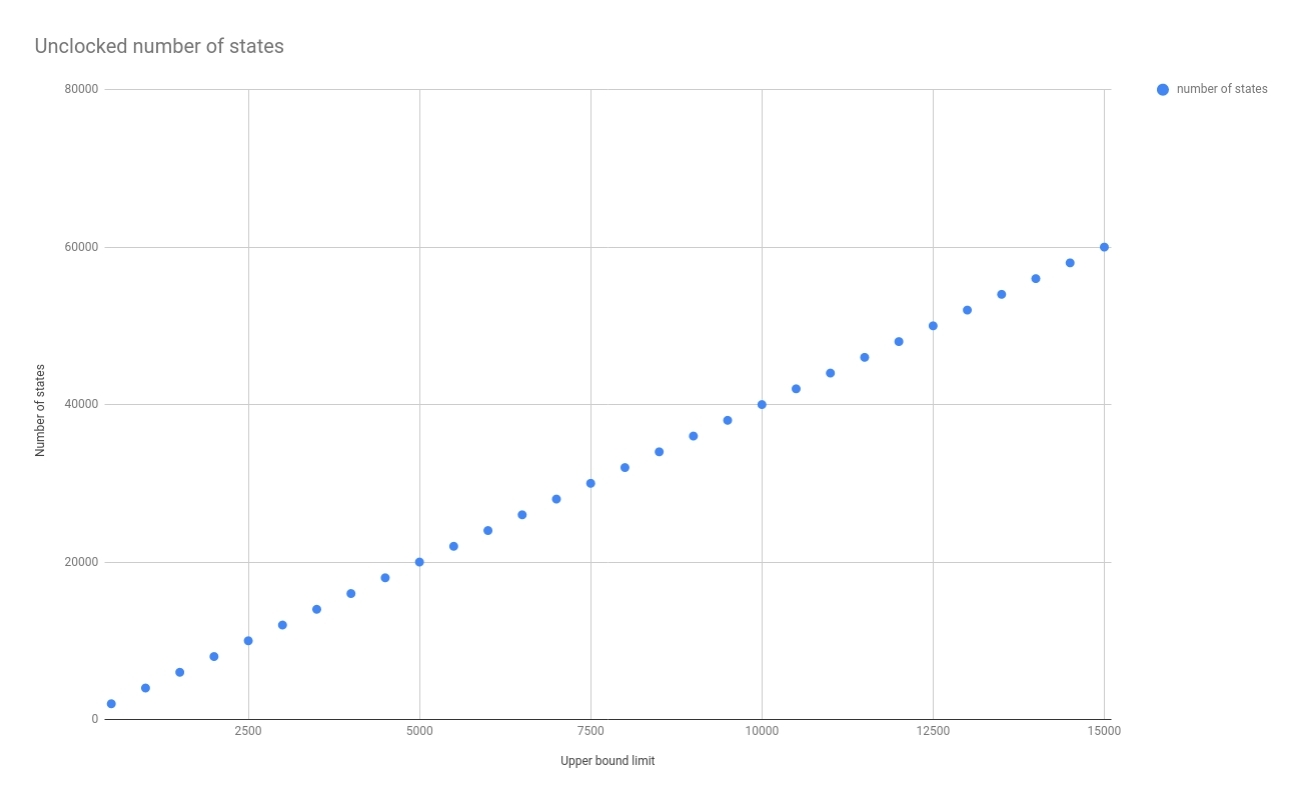
\includegraphics[width=0.98\textwidth]{./figures/temporary_graphs/unclocked_number_of_states.jpg}
\caption{Graph of the \texttt{number of visited states} property from the unclocked seven segments experiment.}
\label{fig:unclocked_states}
\end{figure}
\paragraph{Verification time}
In Figure \ref{fig:unclocked_verification} the \texttt{verification time} results can be seen. The graph represents the verification time in seconds for each increase in the input range. As can be seen the verification time increase exponentially with the input values. Since the number of states visited is increasing linearly it can seem odd that the verification time does not follow that same pattern. However, besides the refinement checking of the GLTS, which will increase with the number of states, FDR4 must compile the network and generate the GLTS. It is reasonable to expect that the larger the state space, the more effort for FDR4 to complete all the steps of the verification. Therefore these results are consistent with what could be expected.
\begin{figure}
    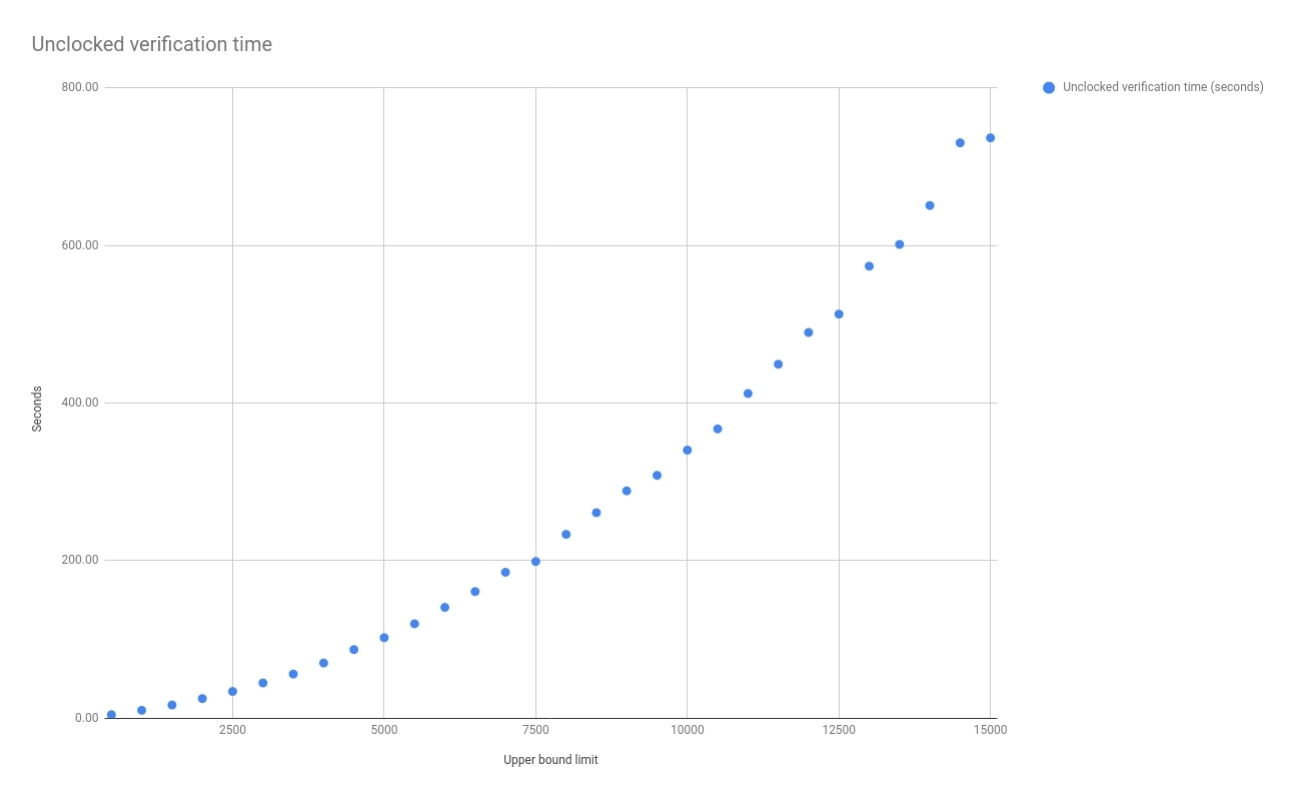
\includegraphics[width=0.98\textwidth]{./figures/temporary_graphs/unclocked_verification_time.jpg}
\caption{Graph of the \texttt{verification time} property from the unclocked seven segments experiment.}
\label{fig:unclocked_verification}
\end{figure}
\paragraph{Maximum resident set size}
The result from this property can be seen in Figure \ref{fig:unclocked_resident_size}. These results are not fitted to a perfect line as well as the other two experiment properties. It is clear that the amount of memory used for the verification grows with an increase in the input range. It is also somewhat consistent until around 10000 in upper bound limit. This fluctuation could be caused by some internal structure in FDR4 or it could be a result of other processes running on the machine that is running the verification. Unfortunately, FDR4 does not provide a lot of information about the internal workings and so it can be very difficult to examine these results further. However, the results are overall consistent with the results from both \texttt{number of visited states} and \texttt{verification time}.
\begin{figure}
    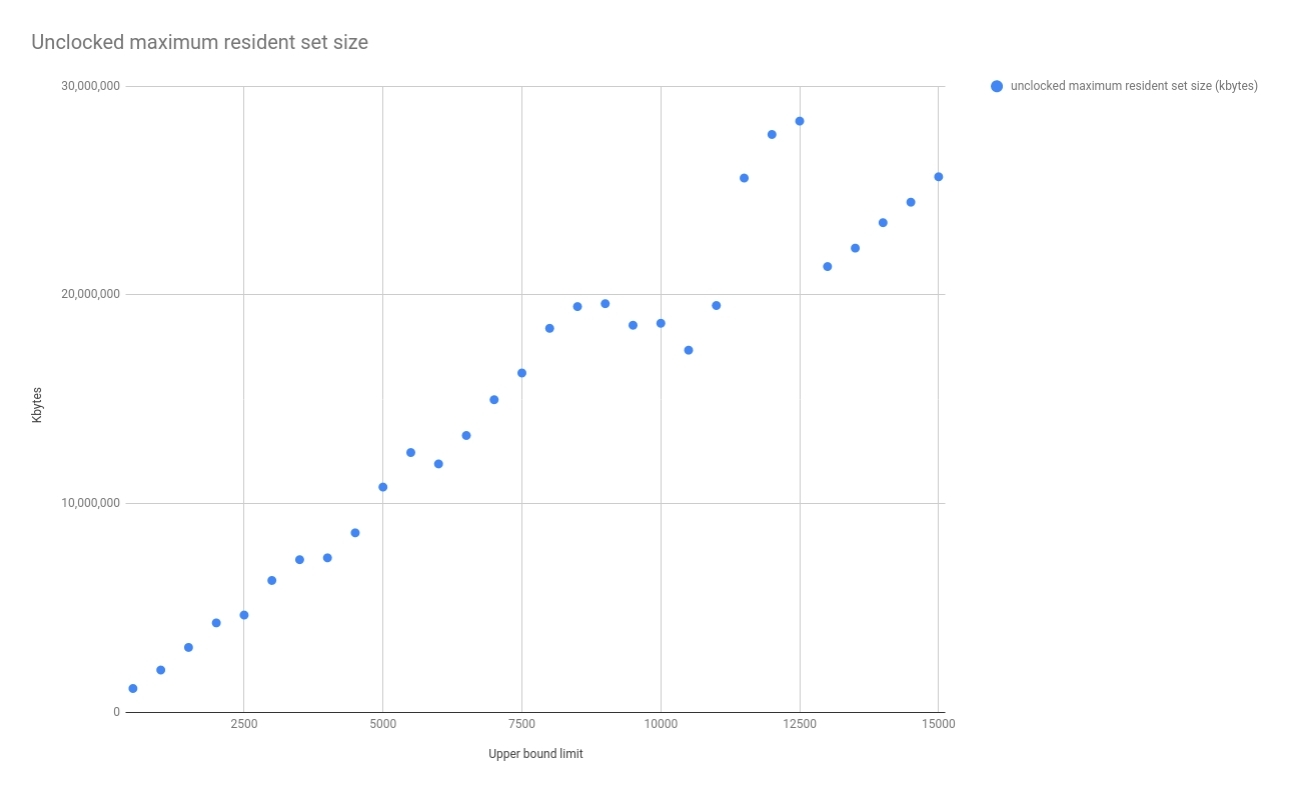
\includegraphics[width=0.98\textwidth]{./figures/temporary_graphs/unclocked_maximum_resident_set_size.jpg}
\caption{Graph of the \texttt{maximum resident set size} property from the unclocked seven segments experiment.}
\label{fig:unclocked_resident_size}
\end{figure}

\subsection{Clocked Experiment}
The full code for the clocked seven segments display example can be seen in Listing \ref{lst:cspm} in Appendix. %TODO: Figure out how this should be presented. One appendix or several?
As in the unclocked seven segments display example, the clocked example also consists of three \texttt{time} processes with associated monitor processes.
In order to make the clocked seven segment experiment equivalent with the unclocked seven segments example, the \texttt{Clock} process in the clocked network only verifies one clock cycle and therefore the two networks should be equivalent in the verification.
\paragraph{Number of visited states}
In Figure \ref{fig:clocked_states}the results of the clocked \texttt{number of visited states} property can be seen for each \texttt{time} verification. As can be seen, they differ quite a lot from each other. The \texttt{number of visited states} property for \texttt{hour} seems to increase every 3600 input increase, and since there are 3600 seconds in one hour, this means that every time the input represents an extra hour, the number of states increase. The \texttt{number of visited states} for \texttt{minutes} increase linearly until exactly 5339 and then stays at 134 for the rest of the verifications. It is very clear from this result that the number of states reaches its maximum when the input range represents the maximum amount of minutes. The input range \{0..5339\} represents 59 minutes which is maximum. The \texttt{number of visited states} for \texttt{seconds} is constant at 134, however if the input range was decreased to \{0..59\} the same result could be seen as with the \texttt{minutes} graph. These results make it clear that FDR4 is able to decrease the number of states to the number of \texttt{hours}, \texttt{minutes} and \texttt{seconds} represented by the input.
\begin{figure}
    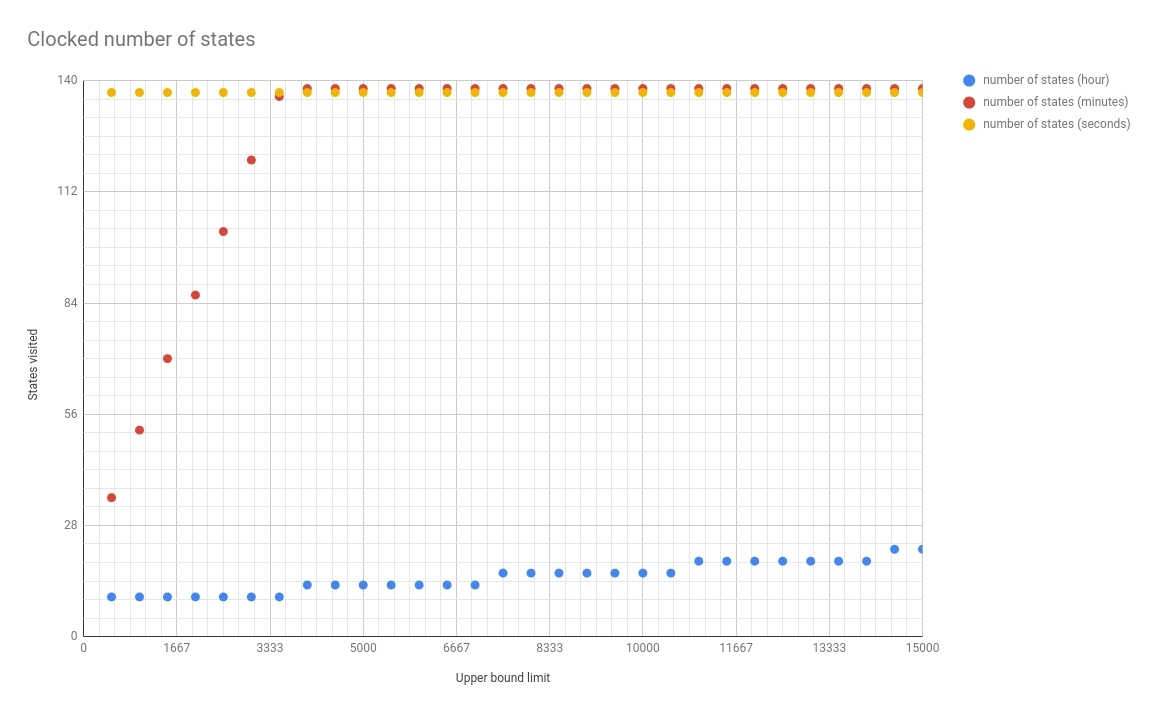
\includegraphics[width=0.98\textwidth]{./figures/temporary_graphs/clocked_number_of_states.jpg}
\caption{Graphs of the three \texttt{number of visited states} properties from the clocked seven segments experiment.}
\label{fig:clocked_states}
\end{figure}
\paragraph{Verification time}
In Figure \ref{fig:clocked_verification} the clocked \texttt{verification time}
results can be seen.
This graph is very similar to the \texttt{verification time} results for the unclocked experiment but with a slightly different increase. However, the values also increase exponentially with the input which, as explained above, is to be expected. What is important to notice is that even though the graph is similar to the unclocked \texttt{verification time} graph, the number of seconds are very different than in the first experiment. The reason for this is probably the decrease in \texttt{number of visited states} which will be discussed further below.
\begin{figure}
    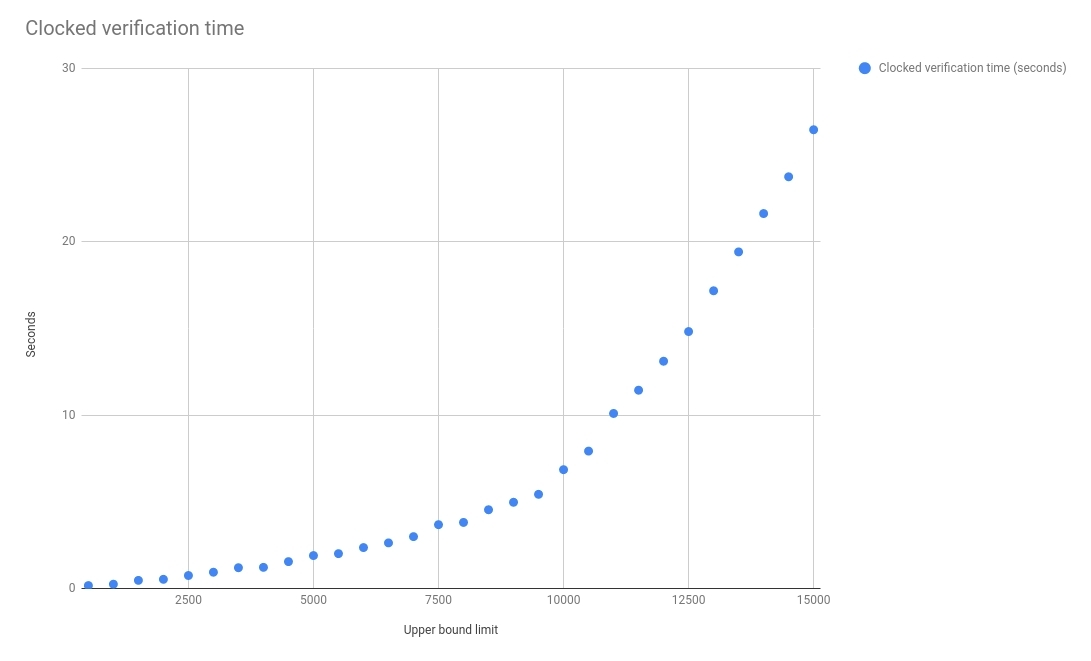
\includegraphics[width=0.98\textwidth]{./figures/temporary_graphs/clocked_verification_time.jpg}
\caption{Graph of the \texttt{verification time} property from the clocked seven segments experiment.}
\label{fig:clocked_verification}
\end{figure}
\paragraph{Maximum resident set size}
Figure \ref{fig:clocked_resident_size} shows the clocked \texttt{maximum resident set size}. This graph shows the same situation as the \texttt{verification time} graph. The graph is similar to that of the unclocked \texttt{maximum resident set size} with a slightly more flattened increase and not nearly as much fluctuation. The big difference with this graph is again the low values compared to the unclocked \texttt{maximum resident set size} values. This is also discussed further below.
\begin{figure}
    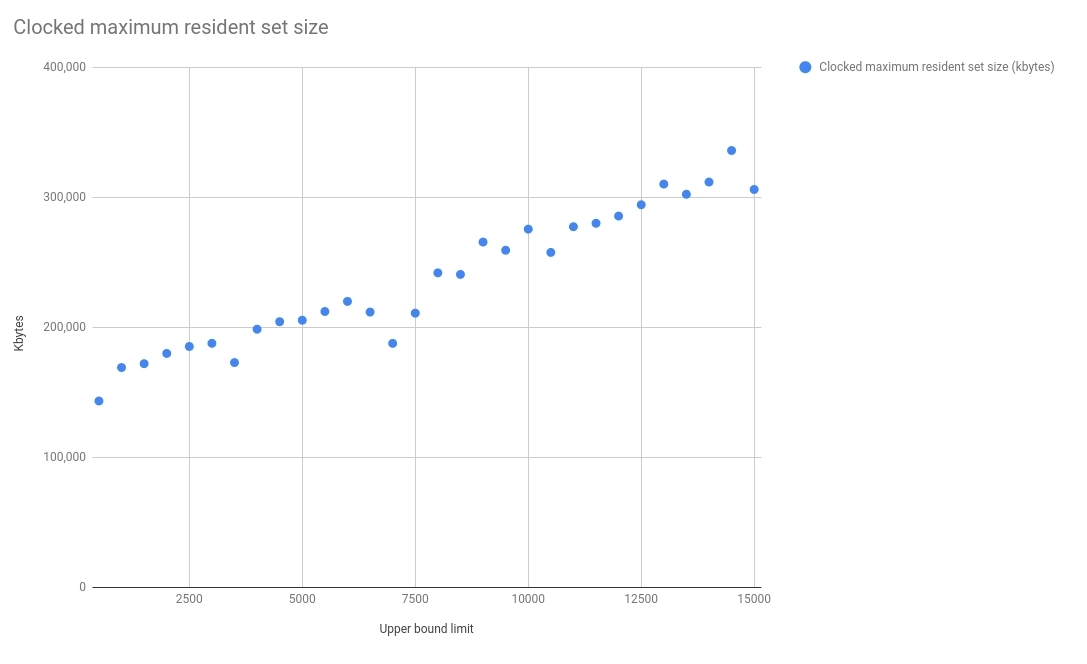
\includegraphics[width=0.98\textwidth]{./figures/temporary_graphs/clocked_maximum_resident_set_size.jpg}
\caption{Graph of the \texttt{maximum resident set size} property from the clocked seven segments experiment.}
\label{fig:clocked_resident_size}
\end{figure}
\subsection{Results}
% TODO when I know I can use this example
As explained above, the \texttt{number of visited states} property from the unclocked seven segments experiment showed to be equal for all three \texttt{time} verifications whereas, for the clocked experiment, the \texttt{number of visited states} varied between the three verifications. Figure \ref{fig:combined_states} represents all four graphs, however, only two can be seen. %TODO: Make sure the new graph used also looks like this.
The reason for this is that the values of the clocked \texttt{number of visited states} are so much lower than the unclocked results that they cannot be shown separately in the graph. \\

In Figure \ref{fig:combined_verification} the combined \texttt{verification time} graph can be seen. Here, the difference also shows very clearly. The clocked experiment verifies much faster than the unclocked. Again it is not possible to display the actual values of the clocked version in the graph because they are too low to be displayed properly. The same case can be seen in Figure \ref{fig:combined_resident_size} which represents the combined \texttt{maximum resident set size}. \\

Both \texttt{verification time} and \texttt{resident set size} seem to be affected by the \texttt{number of visited states} property. This is evident because the
\texttt{number of visited states} is the only internal FDR4 property of the experiment. Unfortunately, it can be quite difficult to investigate why the clocked experiment performs so much better than the unclocked. When looking at the trace of both networks within FDR4, both verify the full input range, as expected. The visualiser ProBE also shows equivalent traces and the two networks behave identically on failures. The only difference between the two networks is that in the clocked system all processes are recursive and synchronise together before continuing. The unclocked processes will always terminate after one clock cycle. However, since the clocked network only simulates one clock cycle, the two networks should still be equivalent. These differences do not affect the actual values verified or the result of the verification. As previously stated when introducing the clocked version of TAPS in Chapter \ref{chap:clock} the increase in complexity might increase the verification time in FDR4, but in this case, it is the opposite. \\

As the two networks seem equivalent in both input range and verification, the reason for the difference in performance might lie in what the \texttt{number of visited states} property shows. It might be that FDR4 is able to compress the state space in the clocked experiment while not being able to perform the same compression in the unclocked experiment. \\

The FDR4 tool provides a machine structure viewer which can provide information about how FDR4 represents the processes and how effective the compression is. When looking at the two different results from FDR4 it becomes clear why the clocked experiment performs so much better than the unclocked experiment. In Figure \ref{fig:unclocked_compression} and Figure \ref{fig:clocked_compression}, the output of the machine structure viewer can be seen. In the unclocked result in Figure \ref{fig:unclocked_compression} the unclocked network
\texttt{N\_hours} is represented by a high-level machine with 12 formats, 77 rules, and 34 leaf machines. A high-level machine means a process with subprocesses and the only information needed about formats and rules are that the more there are, the more complex the machine. \\

Because all events are hidden in the network, as explained in Chapter \ref{chap:design}, the subprocesses are \texttt{Unknown}. The second to last line shows that the compression algorithm \texttt{sbisim} have been applied to \texttt{Hours(0)} but it also shows that it was not able to reduce the number of states or transitions. \\

Figure \ref{fig:clocked_compression} represents the clocked network and, as can be seen, the \texttt{N\_hours} process includes compression information. It provides an estimate that the reduced machine is around 17\% the size of the original machine. On the second to last line, it can be seen that the \texttt{sbisim} compression algorithm is not applied to \texttt{Hours(0)} as in the unclocked experiment, but to \texttt{Hours(..)}. The \texttt{sbisim} compression algorithm is able to compress the state space from 36 states to 6 states. It clearly shows that because FDR4 is able to perform compression on the clocked system, the performance also increases dramatically.\\

It is quite surprising that the clocked experiment have such a drastic difference and that it actually performs better than the unclocked version. As the network increase in complexity the state space should also increase, and it is only because of the compression that the clocked version performs so well. It is, however, not possible to learn exactly why FDR4 is able to perform compression on the clocked network and not on the unclocked. There is a lot of different aspects the way FDR4 structures the network and generate the GLTS. Somehow the clocked network is structured in a way that fits better into the compression algorithm than the unclocked network.
\begin{figure}
    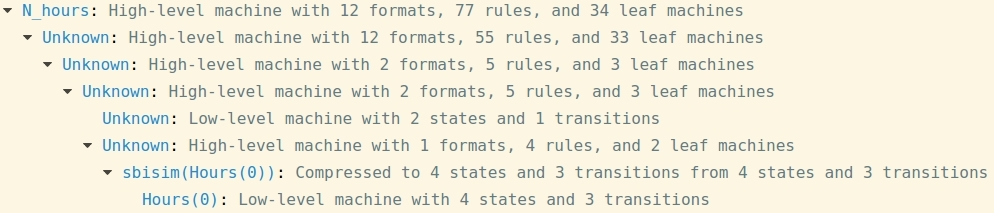
\includegraphics[width=0.98\textwidth]{./figures/unclocked_compression.jpg}
\caption{Screen dump of the results of the unclocked network in the FDR4 machine structure viewer.}
\label{fig:unclocked_compression}
\end{figure}
\begin{figure}
    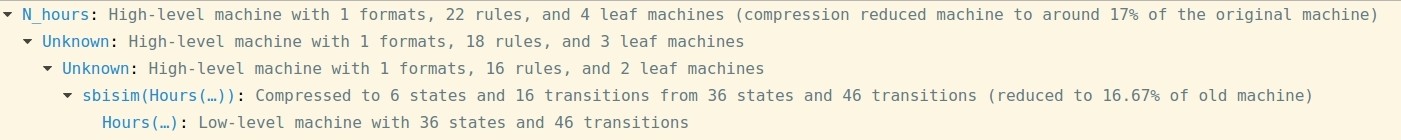
\includegraphics[width=0.98\textwidth]{./figures/clocked_compression.jpg}
\caption{Screen dump of the results of the clocked network in the FDR4 machine structure viewer.}
\label{fig:clocked_compression}
\end{figure}

\begin{figure}
    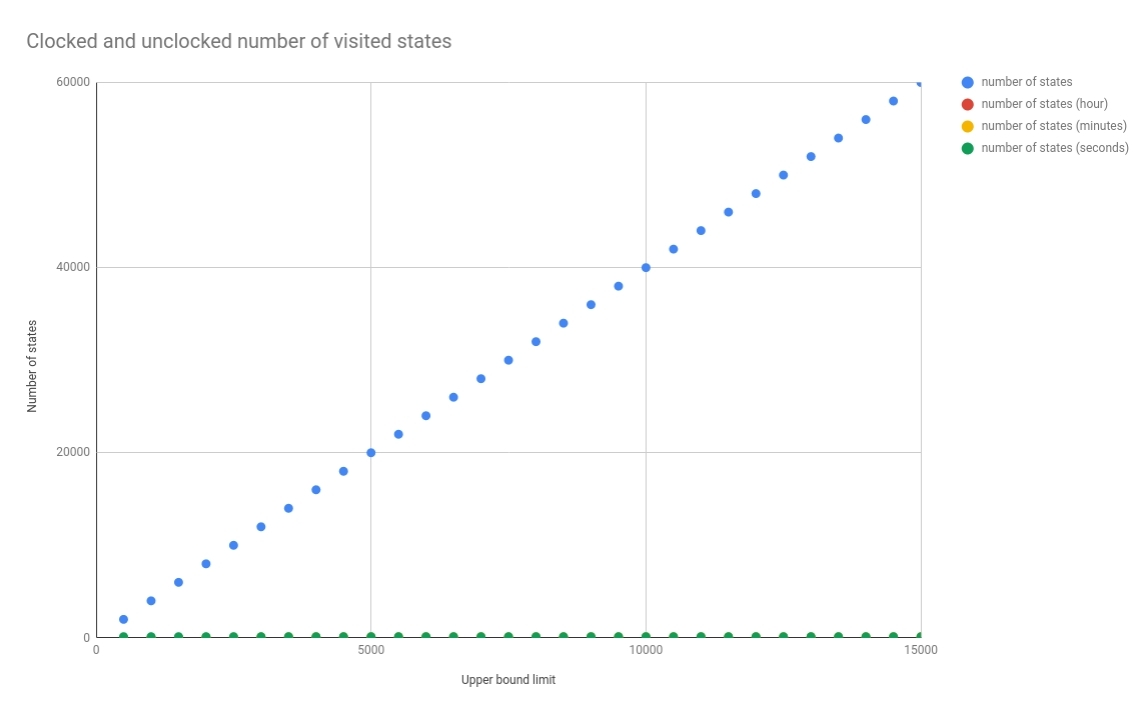
\includegraphics[width=0.98\textwidth]{./figures/temporary_graphs/combined_number_of_states.jpg}
\caption{Graphs of the \texttt{number of states} properties combined from both the unclocked and clocked seven segments experiment.}
\label{fig:combined_states}
\end{figure}

\begin{figure}
    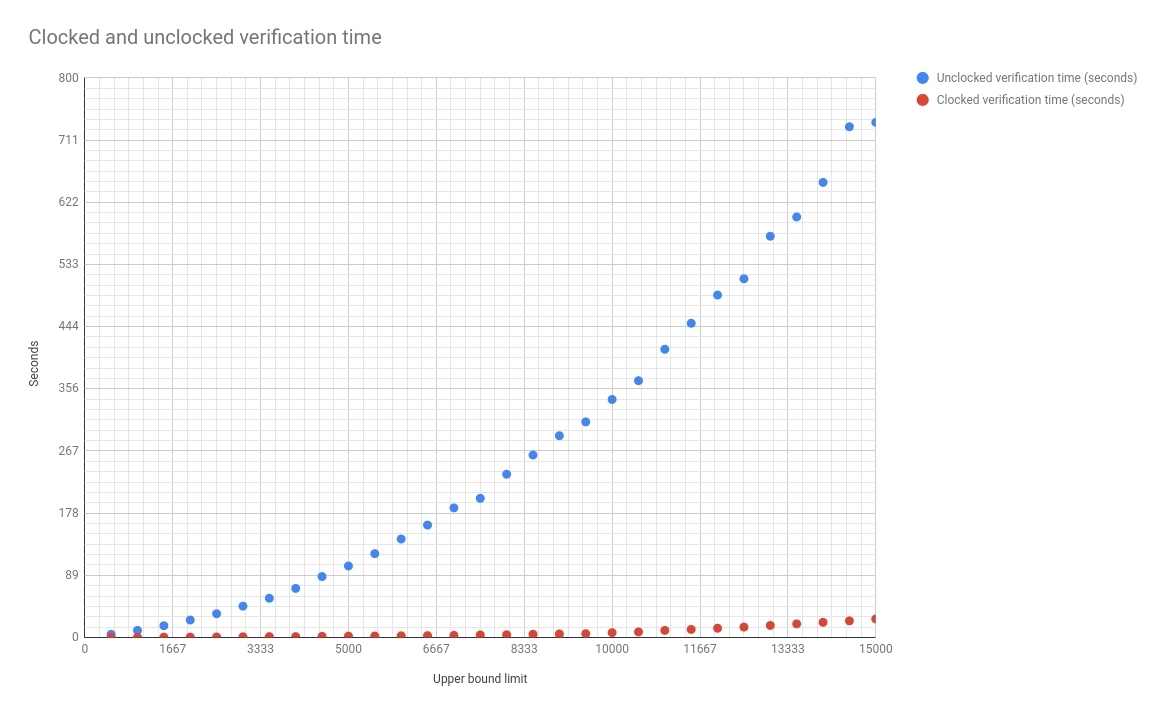
\includegraphics[width=0.98\textwidth]{./figures/temporary_graphs/combined_verification_time.jpg}
\caption{Graphs of the \texttt{verification time} properties combined from both the unclocked and clocked seven segments experiment.}
\label{fig:combined_verification}
\end{figure}

\begin{figure}
    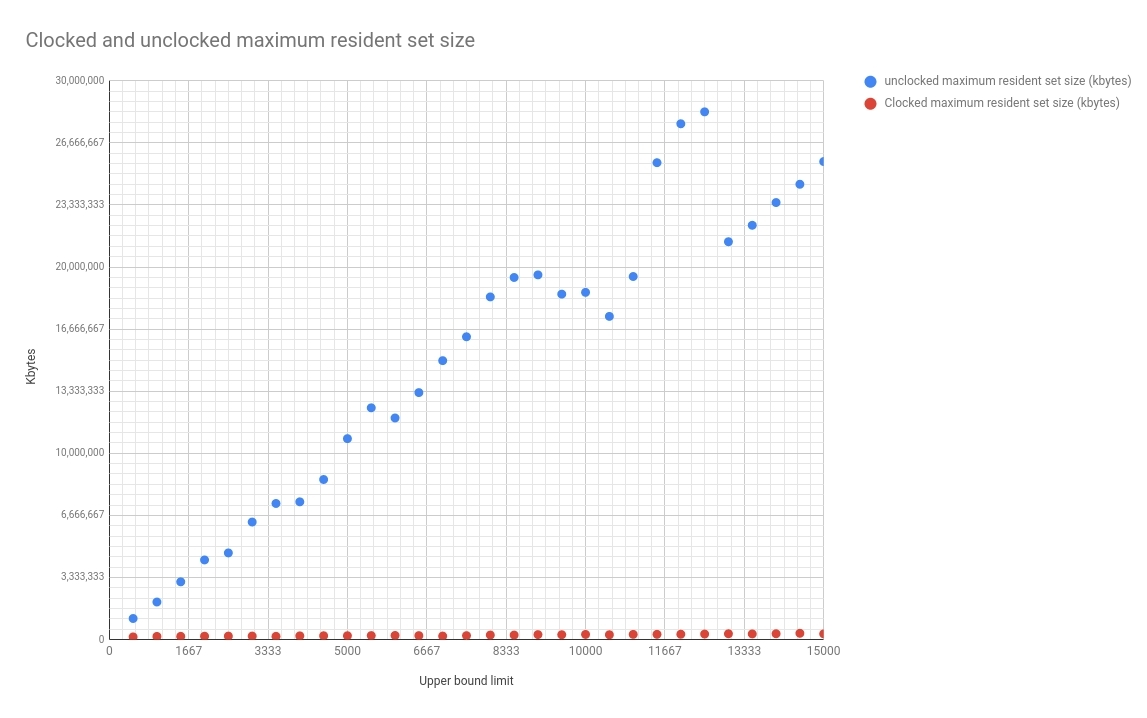
\includegraphics[width=0.98\textwidth]{./figures/temporary_graphs/combined_maximum_resident_set_size.jpg}
\caption{Graphs of the \texttt{maximum resident size set} properties combined from both the unclocked and clocked seven segments experiment.}
\label{fig:combined_resident_size}
\end{figure}




% TODO: I should also still mention something about how the increase in number of processes was or was not feasible.



\newpage
\section{How to use TAPS}
The required dependencies for generating the ANTLR4 parser, running TAPS and verification with FDR4 are listed below:
\begin{itemize}
    \item ANTLR4
    \item Python 2.7
    \item ANTLR Python runtime
    \item FDR4
\end{itemize}

ANTLR4 and FDR4 can both be downloaded from their websites where installation instructions are also provided.
The ANTLR4 project can be found at \url{https://www.antlr.org/} and the FDR4 Project at \url{https://www.cs.ox.ac.uk/projects/fdr/}.\\
It is also necessary to download the ANTLR4 Python runtime from \url{https://pypi.org/project/antlr4-python2-runtime/}.
Assuming that an ANTLR4 alias has been created as the ANTLR4 installation suggest, the parser and lexer can be generated with ANTLR4 using the command: {\ttfamily antlr4 -Dlanguage=Python2 - visitor -no-listener Smeil.g4.}
This will create all the required parser and lexer files as well as the visitor methods. This step is only necessary if the .g4 grammar file has been modified.\\

When the ANTLR4 files have been generated TAPS can be used directly with a well-formed SMEIL program with the command: {\ttfamily python taps.py input.sme output.csp}. The system requires both an input file as well as an output file. If the output file does not exist it will be created by TAPS. \\

The resulting \cspm{} file can be verified in FDR either by the command line tool or by the FDR4 tool which is a graphical tool. The command line tool can be used by the command \texttt{refines output.csp}. There are several options to adjust the output of the command. The FDR4 command line tool is mostly used to quickly check if a network passes the verification because it is difficult to navigate the counterexamples. The FDR4 graphical tool provides a better visualisation of counterexamples and the ProBE visualiser can be called directly from the FDR graphical tool.



% \chapter{Discussion}
% \label{chap:discussion}
% %!TEX root = ../main.tex
In this chapter, I will discuss the usability of TAPS and how the clocked version increases the set of verifiable problems. I will also discuss how TAPS currently only allows translation of pure SMEIL networks, and how TAPS can be extended for co-simulation. Lastly, I will discuss the advantages and limitations of the FDR4 tool.
\section{Usability of TAPS}
TAPS have proven to be a capable tool for automatic translation from SMEIL to \cspm{}. It is still in early stages of development and more examples must be developed and verified, in order to handle more aspects of the SMEIL language.\\

To my knowledge, transpiling from a hardware description language to a specification language like CSP has not been done successfully before, and the advantages of such a system are many. When using TAPS, it is not necessary to develop a test bench for the system, and it is not necessary to develop the specification model separately from the hardware model. This means that the workflow from developing the hardware model to verifying it, has been simplified dramatically with TAPS. I believe that being able to perform verification with no extra development steps will increase the attractiveness of SME for hardware development and further its advantage over traditional HDLs.\\

There are limitations to TAPS and it is still possible for failures to happen with systems verified with TAPS. The bottlenecks of the verification lie both in the observed values as well as in the number of verified clock cycles.

The values verified in FDR4 are based on the observed values from the simulation, so if the SMEIL simulation does not represent all possible values, the verification will be incomplete.
It is difficult to find a balance between how long to simulate the SMEIL network and how critical failures can be. In some systems it will not be possible to know when all corner cases have been found in the simulation, however, FDR4 might provide insight into some corner cases missing in the simulation.
% TODO: Do I want to keep this?
It is possible for the developer to bypass the simulation step and hardcode the observed values directly. The SMEIL program must still be well-formed for TAPS to translate it, but the developer can specify specific data if needed without depending on the simulation. However, it might prove to be more difficult for the developer to specify values that represent the entire possible input range.\\

In clocked version of TAPS additional information must be provided to the system. The user must define the number of clock cycles to verify, which bring more uncertainty to the verification. If the user chooses too few clock cycles to verify, potential failures might not be caught by FDR4. The number of clock cycles to verify is a balance between the input range for the system, the time requirement of the verification, as well as the complexity of the system.
The user must ultimately determine the balance between verification and verification time, based on the program at hand. \\

The reason that it is possible to create the relatively simple translations from SMEIl to \cspm{}, lies in the fact that SME is defined from the CSP model and therefore, as previously mentioned, all SME models will have an equivalent CSP model. Having the same basis on both sides of the translation results in a much smoother translation.

\section{Clocked or Unclocked \cspm{} Systems}
The initial idea for the design of TAPS was to build a system which did not have to enforce a global synchronous clock structure, since it would increase the complexity drastically. As the implementation of the initial version of TAPS progressed, it was clear that the design was too simple. The set of verifiable problems in the initial version of TAPS are too small to have an actual impact.
The clocked version of TAPS is still able to verify the set of problems verifiable with the initial version of TAPS. By only verifying one clock cycle, the results are the same as for the unclocked version of TAPS.
It is, of course, an advantage that the new design only adds to the set of verifiable problems, and doesn't reduce it.\\

It is a huge advantage that the clocked TAPS system is able to reuse such a large part of the initial design. It was possible to extend the initial version of TAPS instead of rewriting the entire system, which also made it feasible to design within the timeframe of this thesis.
It is also clear that the set of verifiable problems with the clocked TAPS system are far bigger than the initial version of TAPS, so there is no doubt that this extension has been an advantage, in spite of the increase in complexity.
The clocked \cspm{} network provides comparability with the original SMEIL network, which I believe is a huge advantage for the further development of TAPS. When developing and testing new features of TAPS, it is a big advantage to be able to compare the behavior of the SMEIL simulation to that of the FDR4 verification. \\

% TODO: Change if I cant have the clocked experiment in the report
From the experiments presented above, it is clear that the clocked structure performs a lot better than the unclocked system, which increases the usability of TAPS. It is, of course, necessary to perform further experiments to see if the compression is possible because of the general clocked structure of the network, or because of the structure of that specific clocked network.
The implementation of the clocked version of TAPS is still in progress, and there are bound to be challenges to the translation structures, which will require some ingenuity to ensure proper code generation.
\section{From Pure SMEIL to Co-Simulation}
Co-simulation is a major feature of SMEIL and yet I only focused on pure SMEIL support in this thesis. The reason for this decision was to have a simple base to start from, to ensure the accuracy of the translations.\\

TAPS should definitely be extended to support translation of co-simulated networks. TAPS will not have any real value to the industry or academia until this happens, because pure SMEIL does not allow for a lot of functionality.
However, I do believe that the extension to support co-simulated programs is possible.\\

The external communication between SMEIL and another SME implementation can be represented in trace files, generated from the simulation. TAPS can use these data as the observed values for the translation. The external channels are defined with the keyword \texttt{exposed}, so TAPS can recognise these, and read the data directly from the corresponding trace file. This way, TAPS would be able to generate a channel range similar to the internal observed values.
It will, of course, be a challenge to handle the data and communication that spans across the SME implementations in co-simulation. However, since it is very precisely defined which buses communicate across the two implementations, and the data communicated can be saved in trace files, it should be possible to implement.\\

Focusing first on pure SMEIL programs have definitely led to a more manageable set of problems, but extending this to co-simulated problems seems like the perfect next step.

\section{Verification with FDR4}
There is no doubt that there lies a huge advantage in the possibility of hardware verification. Failures in critical systems can be disastrous and testing simply does not provide the security needed for these types of systems. FDR4 is a solid system and the addition of the ProBE visualiser within FDR4 is a huge advantage to provide an understanding of the network, but FDR4 does have its limitations. Even though it is relatively simple to verify a network in FDR4, the counterexamples can be challenging to understand, depending on the network. Understanding the different aspects and functionality of FDR4, requires the user to know a substantial amount about the structures of CSP. This means that the requirement of understanding CSP is not entirely obsolete when using TAPS. The developer does not need to model the specification manually, but verifying it requires some CSP knowledge. The need to have a basic knowledge of CSP occurs for example in the debug viewer. Here, a process that terminates successfully ends the trace with the symbol $\tick$. Processes that deadlocks or behaves as the \texttt{STOP} process are defined with the symbol $\nullset$. These two symbols are standard syntax in CSP, but not for \cspm{}. This means that if the user does not have any knowledge in CSP, it can be difficult to understand the debug viewer since it uses different symbols than used in the verified \cspm{} program. Therefore the user must have a basic knowledge of CSP to utilise all the different possibilities of FDR4. \\

% TODO: Change if I cannot have clocked experiement in report
With FDR4, as with every other model checking, the size of the state space is a bottleneck that can hinder the verification of larger problems. FDR4 performs state space compression and it also provides several compression algorithm functions to apply directly within the \cspm{} network.
However, it is essential that the verification time is manageable, and for networks like the unclocked seven segments display network, this is not the case. As it is clear from the results in Chapter \ref{chap:exp}, a network can quickly grow to a point where verification is infeasible due to time constraints. This is, however, a general problem with model checking and it is an active research area that keeps improving.
% %
% \chapter{Future Work}
% \label{chap:future}
% %!TEX root = ../main.tex

Different SME implementations is in active development and so the SMEIL language will be extended and improved to match the new features of the different SME implementations. As the SMEIL language becomes more comprehensive and supports more features, TAPS should be kept in line with the advancements of SMEIL.\\
The automatic verification provided by TAPS, decrease a mayor workload in testing and verifying hardware models in the SME model and therefore, it is also relevant to structure the SMEIL implementation towards better FDR4 results, while still maintaining the basic SME model structure. \\

The extended version of TAPS provides an extended verification of the different internal states within a hardware model. It was introduced rather late in the project and therefore the development have not been as extensive as the initial version of TAPS. A substantial groundwork have been laid in providing the design structures for the extended version, making further development more straightforward. It is, however, obvious that future work should include providing a full implementation of the extended TAPS system. \\

Besides further development of the extended version of TAPS, more advanced and in-depth examples should be developed in SMEIL in order to understand the limitations of the translation as well as FDR4.\\

FDR4 also provides the possibility of integration with other tools using the FDR4 API which is currently available for C++, Java and Python. The FDR4 API is currently not used in TAPS, but it is an obvious choice to extend TAPS to use the FDR4 API to provide a more clean workflow. Because TAPS have been developed for FDR4 specifically, no other verification tool will match the current translation structures and therfore the current version of TAPS would benefit from the available API.\\

As described in Chapter \ref{chap:background}, SMEIL was mainly developed to provide co-simulation with other SME implementations. TAPS should be augmented to support co-simulation. The optimal solution would be for TAPS to provide translations from other SME implementations as well as SMEIL, in order to translate the entire co-simulated network into \cspm{}. A simpler solution would be to translate the SMEIL code of the co-simulation along with the data representing the communication between the different SME implementations. This solution would not provide verification for the total network but it is very similar to the pure SMEIL translation that TAPS can currently provide.\\


Another point for future work is to extend the different assertion possibilities within TAPS. Currently only channel communication can be verified, but as described in Chapter \ref{chap:implementation} %TODO: Make sure I have written this!
these monitor processes does have its limitations because each monitor process can verify a value, but it is not currently possible to verify the combination of values. Therfore it would be an advantage to extend TAPS to define more advanced assertions to verify values over multiple channels. \\

In future work, it would be an advantage to extend TAPS to support software-hardware co-design. The idea behind software-hardware co-design is that hardware and software is designed in parallel so that both can be implemented on either hardware or software depending on what is most suited. If SMEIL and TAPS was extended to support this, then the communication between software and hardware would be possible to verify with FDR4. \\

When verifying a system in FDR4, it can be crucial for the developer to know what values and states have been verified. It is therefore desirable to have TAPS generate a human-readable report on the ranges and communications that are verified with TAPS. This would also give the developer a possibility of better evaluating the number of clock cycles to verify in FDR4.
This report could become a standard addition to the documentation of the developed system, which would give a programmer an easy overview of a complicated system and would also allow for easier contemplation over the system.
%
\chapter{Conclusion}
%!TEX root = ../main.tex
In this thesis, I have presented TAPS, a transpiler that translates programs written in the
new SME intermediate language (SMEIL) into the machine-readable CSP language (\cspm{}). In TAPS, the translated \cspm{} code is augmented with assertion
properties which can be verified with the Failure-Divergences Refinement tool
(FDR4).\\

I have presented an initial system, which is able to translate SMEIL networks to
\cspm{}, and verify a large range of defined input values. TAPS can assert that
the observed values of a channel in a simulated SMEIL program are in fact the
only possible values communicated on that specific channel. \\

An extension to the initial version of TAPS has also been presented in this
thesis. This extension provides TAPS with the support to model a global
synchronous clock in \cspm{}. It has previously been shown~\cite{Skaarup14}
that enforcing a global synchronous clock onto a PyCSP network results in code complexity explosion. To avoid having to model networks with an enormous amount of
states, the SME model was developed, based on the CSP algebra. With the
extended version of TAPS, the state explosion still occurs, but because TAPS automatically generates the \cspm{} code, the state explosion is not a hindrance to the
translation.\\

The translated \cspm{} network can be verified with the FDR4 tool, which can
perform refinement checks on \cspm{} networks. I present examples of failures
and solution to these with an example of a seven segment display network and a
cyclic "addone" network, showing the advantages of both the initial version of TAPS, and the clocked version.\\

This system makes it more accessible for software programmers to program
hardware, thereby bridging a gap between software programmers and the needs
of the industry.
Instead of having to create advanced test-benches, TAPS provides a simple
way to verify the hardware model via the assertion functionalities of FDR4.
TAPS does not yet provide support for the entire SMEIL language. In spite of this,
I am pleased with the possibilities that TAPS present, and I have shown the current capabilities of TAPS are valuable.\\

Part of this work has been published in the paper \textit{Towards Automatic Program Specification Using SME Models}~\cite{TheglerEtAl2018}, which is included in full length in Appendix \ref{app:paper}. The extended clocked version of TAPS was designed subsequently.


% \chapter*{Acknowledgements}
% % Thanks to Uwe Zimmermann who made the seven segment example in TikZ on \url{http://www.texample.net/tikz/examples/segment-display/}.


\newpage
citation for citations\cite{Bengtsson1995}


%%%%%%%%%%%%%%%%
% Bibliography %
%%%%%%%%%%%%%%%%

% \clearpage
% \addcontentsline{toc}{chapter}{References}
% \printbibliography[title={References}]

\newpage
\bibliographystyle{abbrv}
\bibliography{library}

%%%%%%%%%%%%%%%%%%%%
% Include Appendix %
%%%%%%%%%%%%%%%%%%%%
% \appendix
% % Appendix
\chapter{How To Use TAPS}
The required dependencies for generating the ANTLR4 parser, running TAPS and verification with FDR4 are listed below:
\begin{itemize}
    \item ANTLR4
    \item Python 2.7
    \item ANTLR Python runtime
    \item FDR4
\end{itemize}

ANTLR4 and FDR4 can both be downloaded from their websites, where installation instructions are also provided.
The ANTLR4 project can be found at \url{https://www.antlr.org/} and the FDR4 Project at \url{https://www.cs.ox.ac.uk/projects/fdr/}.
It is also necessary to download the ANTLR4 Python runtime from \url{https://pypi.org/project/antlr4-python2-runtime/}.
Assuming that an ANTLR4 alias has been created as the ANTLR4 installation suggest, the parser and lexer can be generated with ANTLR4 using the command: {\ttfamily antlr4 -Dlanguage=Python2 - visitor -no-listener Smeil.g4.}
This will create all the required parser and lexer files, as well as the visitor methods. This step is only necessary if the .g4 grammar file has been modified.\\

When the ANTLR4 files have been generated, TAPS can be used directly with a well-formed SMEIL program with the command: {\ttfamily python taps.py input.sme output.csp}. The system requires both an input file and an output file. If the output file does not exist, it will be created by TAPS. \\

The resulting \cspm{} file can be verified in FDR4, either by the command line tool or by the FDR4 tool, which is a graphical tool. The command line tool can be used by the command \texttt{refines output.csp}. There are several options to adjust the output of the command. The FDR4 command line tool is mostly used to quickly check if a network passes the verification, because it is difficult to navigate the counterexamples. The FDR4 graphical tool provides a better visualisation of counterexamples, and the ProBE visualiser can be called directly from the FDR4 graphical tool.

\chapter{Seven Segments Display Example Full Code}
\label{app:seven_segments}
\section*{SMEIL Code}
\begin{minted}{smeil_lexer.py:SMEILLexer -x}
proc clock ()
    bus clock_out {val: u17 range 1 to 86401;};
    var i: u17 = 0 range 0 to 86401;
{
    i = i + 1;
    clock_out.val = i;
}


proc hours (in hours_in)
    bus hours_out {first_digit: u2 range 0 to 2;
                   second_digit: u4 range 0 to 9;};
    var hours: u5 range 0 to 23;
    var hours_first_temp: u2 range 0 to 2;
    var hours_second_temp: u4 range 0 to 9;
{
    hours = hours_in.val / 3600 % 24;
    hours_first_temp = hours / 10;
    hours_second_temp = hours % 10;
    hours_out.first_digit = hours_first_temp;
    hours_out.second_digit = hours_second_temp;
}


proc minutes (in minutes_in)
    bus minutes_out {first_digit: u3 range 0 to 5;
                     second_digit: u4 range 0 to 9;};
    var minutes: u6 range 0 to 59;
    var minutes_first_temp: u3 range 0 to 5;
    var minutes_second_temp: u4 range 0 to 9;

{
    minutes = minutes_in.val / 60 % 60;
    minutes_first_temp = minutes / 10;
    minutes_second_temp = minutes % 10;
    minutes_out.first_digit = minutes_first_temp;
    minutes_out.second_digit = minutes_second_temp;
}


proc seconds (in seconds_in)
    bus seconds_out {first_digit: u3 range 0 to 5;
                     second_digit: u4 range 0 to 9;};
    var seconds: u6 range 0 to 59;
    var seconds_first_temp: u3 range 0 to 5;
    var seconds_second_temp: u4 range 0 to 9;
{
    seconds = seconds_in.val % 60;
    seconds_first_temp = seconds / 10;
    seconds_second_temp = seconds % 10;
    seconds_out.first_digit = seconds_first_temp;
    seconds_out.second_digit = seconds_second_temp;
}


network clock_network ()
{
    instance g of clock();
    instance h of hours(g.clock_out);
    instance m of minutes(g.clock_out);
    instance s of seconds(g.clock_out);
}

\end{minted}
\captionof{listing}{The full SMEIL code used for transpiling in the seven segment display example.\label{lst:smeil}}

\section*{Unclocked \cspm{} Code}
\begin{minted}{cspm_lexer.py:CSPmLexer -x}
channel clock_out_val : {0..131071}

channel hours_out_first_digit : {0..3}
channel hours_out_second_digit : {0..15}

channel minutes_out_first_digit : {0..7}
channel minutes_out_second_digit : {0..15}

channel seconds_out_first_digit : {0..7}
channel seconds_out_second_digit : {0..15}


Hours(hours_in) =
let
    hours = hours_in / 3600  % 24
    hours_first_temp = hours / 10
    hours_second_temp = hours % 10
within
    hours_out_first_digit ! hours_first_temp ->
    hours_out_second_digit ! hours_second_temp ->
    SKIP

Hours_out_first_digit_monitor(c) =
    c ? x ->
    (0 <= x and x <= 2) & SKIP
Hours_out_second_digit_monitor(c) =
    c ? x ->
    (0 <= x and x <= 9) & SKIP


Minutes(minutes_in) =
let
    minutes = minutes_in / 60  % 60
    minutes_first_temp = minutes / 10
    minutes_second_temp = minutes % 10
within
    minutes_out_first_digit ! minutes_first_temp ->
    minutes_out_second_digit ! minutes_second_temp ->
    SKIP

Minutes_out_first_digit_monitor(c) =
    c ? x ->
    (0 <= x and x <= 5) & SKIP
Minutes_out_second_digit_monitor(c) =
    c ? x ->
    (0 <= x and x <= 9) & SKIP


Seconds(seconds_in) =
let
    seconds = seconds_in % 60
    seconds_first_temp = seconds / 10
    seconds_second_temp = seconds % 10
within
    seconds_out_first_digit ! seconds_first_temp ->
    seconds_out_second_digit ! seconds_second_temp ->
    SKIP

Seconds_out_first_digit_monitor(c) =
    c ? x ->
    (0 <= x and x <= 5) & SKIP
Seconds_out_second_digit_monitor(c) =
    c ? x ->
    (0 <= x and x <= 9) & SKIP


N_hours = clock_out_val ? variable ->
          (Hours(variable)
          [| {| hours_out_first_digit|} |]
          Hours_out_first_digit_monitor(hours_out_first_digit))
          [| {| hours_out_second_digit|} |]
          Hours_out_second_digit_monitor(hours_out_second_digit)

assert SKIP [F= N_hours \ Events


N_minutes = clock_out_val ? variable ->
            (Minutes(variable)
            [| {| minutes_out_first_digit|} |]
            Minutes_out_first_digit_monitor(minutes_out_first_digit))
            [| {| minutes_out_second_digit|} |]
            Minutes_out_second_digit_monitor(minutes_out_second_digit)

assert SKIP [F= N_minutes \ Events


N_seconds = clock_out_val ? variable ->
            (Seconds(variable)
            [| {| seconds_out_first_digit|} |]
            Seconds_out_first_digit_monitor(seconds_out_first_digit))
            [| {| seconds_out_second_digit|} |]
            Seconds_out_second_digit_monitor(seconds_out_second_digit)

assert SKIP [F= N_seconds \ Events

\end{minted}
\captionof{listing}{The full unclocked \cspm{} code after transpiling the seven segment display example, as seen in Listing~\ref{lst:smeil} in Appendix \ref{app:seven_segments}.\label{lst:cspm}}
\section*{Clocked \cspm{} Code}
\begin{minted}{cspm_lexer.py:CSPmLexer -x}
channel hours_hours_out_first_digit : {0..3}
channel hours_hours_out_second_digit : {0..15}
channel minutes_min_out_first_digit : {0..7}
channel minutes_min_out_second_digit : {0..15}
channel seconds_sec_out_first_digit : {0..7}
channel seconds_sec_out_second_digit : {0..15}
channel clock_c_out_val : { 0..1000}
channel sync

Clock(1) = SKIP
Clock(n) =  sync -> sync -> Clock(n+1)

Hours(input_channel) =
    (sync ->
     input_channel ? hours_in ->
     sync ->
        let
            hours = ( hours_in / 3600 ) % 24
            hours_first_temp = hours / 10
            hours_second_temp = hours % 10
        within
            (hours_first_temp <= 3) &
                (hours_hours_out_first_digit ! hours_first_temp ->
                (hours_second_temp <= 15) &
                    (hours_hours_out_second_digit ! hours_second_temp ->
                    Hours(input_channel)
                    )
                )
    ) [] SKIP

hours_hours_out_first_digit_monitor(c) =
    (c ? x ->
    (0 <= x and x <= 2 or x == -1) &
        hours_hours_out_first_digit_monitor(c)
    ) [] SKIP

hours_hours_out_second_digit_monitor(c) =
    (c ? x ->
    (0 <= x and x <= 9 or x == -1) &
        hours_hours_out_second_digit_monitor(c)
    ) [] SKIP


N_hours =
        (
            (
                Hours(clock_c_out_val)
                [|{| hours_hours_out_first_digit |}|]
                hours_hours_out_first_digit_monitor(hours_hours_out_first_digit)
            )
            [|{| hours_hours_out_second_digit |}|]
            hours_hours_out_second_digit_monitor(hours_hours_out_second_digit)
        )
        [|{| sync |}|]
        Clock(0)

assert SKIP [F= N_hours \ Events


Minutes(input_channel) =
    (sync ->
     clock_c_out_val ? min_in ->
     sync ->
        let
            min = ( min_in / 60 ) % 60
            min_first_temp = min / 10
            min_second_temp = min % 10
        within
            (min_first_temp <= 7) &
                (minutes_min_out_first_digit ! min_first_temp ->
                (min_second_temp <= 15) &
                    (minutes_min_out_second_digit ! min_second_temp ->
                    Minutes(input_channel)
                    )
                )
    ) [] SKIP

minutes_min_out_first_digit_monitor(c) =
    (c ? x ->
    (0 <= x and x <= 5 or x == -1) &
        minutes_min_out_first_digit_monitor(c)
    ) [] SKIP

minutes_min_out_second_digit_monitor(c) =
    (c ? x ->
    (0 <= x and x <= 9 or x == -1) &
        minutes_min_out_second_digit_monitor(c)
    ) [] SKIP

N_minutes =
        (
            (
                Minutes(clock_c_out_val)
                [|{| minutes_min_out_first_digit |}|]
                minutes_min_out_first_digit_monitor(minutes_min_out_first_digit)
            )
            [|{| minutes_min_out_second_digit |}|]
            minutes_min_out_second_digit_monitor(minutes_min_out_second_digit)
        )
        [|{| sync |}|]
        Clock(0)

assert SKIP [F= N_minutes \ Events


Seconds(input_channel) =
    (sync ->
     clock_c_out_val ? sec_in ->
     sync ->
        let
            sec = sec_in % 60
            sec_first_temp = sec / 10
            sec_second_temp = sec % 10
        within
            (sec_first_temp <= 7) &
                (seconds_sec_out_first_digit ! sec_first_temp ->
                (sec_second_temp <= 15) &
                    (seconds_sec_out_second_digit ! sec_second_temp ->
                    Seconds(input_channel)
                    )
                )
    ) [] SKIP


sec_sec_out_first_digit_monitor(c) =
    (c ? x ->
    (0 <= x and x <= 5) &
        sec_sec_out_first_digit_monitor(c)
    ) [] SKIP

sec_sec_out_second_digit_monitor(c) =
    (c ? x ->
    (0 <= x and x <= 9) &
        sec_sec_out_second_digit_monitor(c)
    ) [] SKIP

N_seconds =
        (
            (
                Seconds(clock_c_out_val)
                [|{| seconds_sec_out_first_digit |}|]
                sec_sec_out_first_digit_monitor(seconds_sec_out_first_digit)
            )
            [|{| seconds_sec_out_second_digit |}|]
            sec_sec_out_second_digit_monitor(seconds_sec_out_second_digit)
        )
        [|{| sync |}|]
        Clock(0)

assert SKIP [F= N_seconds \ Events
\end{minted}
\captionof{listing}{The full clocked \cspm{} code after transpiling the seven segment display example, as seen in Listing~\ref{lst:smeil} in Appendix \ref{app:seven_segments}.\label{lst:cspm_clocked}}


\chapter{Addone Example Full \cspm Code}
\label{app:addone}
\section*{\cspm{} Code}
\begin{minted}{cspm_lexer.py:CSPmLexer -x}
channel sync
channel d_read, c_read : { -1..15} -- u4 and initial value
channel d_write, c_write : { -1..15} -- u4 and initial value

DUM_VAL = -1 -- initial value


Add(i, input_channel) =
    (sync ->
     input_channel ? x ->
     sync ->
        if (x == DUM_VAL) -- initial value
            then (
                let
                    var = i
                within
                    var <= 15 & -- upper limit
                        c_read ! var -> Add(i, input_channel))
            else (
                let
                    var = (x + 1) % 11 -- observed value + 1 restriction
                within
                    var <= 15 & -- upper limit
                        c_read ! var -> Add(i, input_channel))
    )
    [] SKIP


Id(i, input_channel) =
    (sync ->
     input_channel ? x ->
     sync ->
        if (x == DUM_VAL) -- initial value
            then (
                i <= 15 & -- upper limit
                    d_read ! i -> Id(i, input_channel))
            else (
                x <= 15 & -- upper limit
                    d_read ! x -> Id(i, input_channel))
    )
    [] SKIP


c_read_monitor(c) =
    (c ? x ->
    (0 <= x and x <= 10 or x == -1) & -- observed values + initial value
        c_read_monitor(c)
    ) [] SKIP

d_read_monitor(c) =
    (c ? x ->
    (0 <= x and x <= 10 or x == -1) & -- observed values + initial value
        d_read_monitor(c)
    ) [] SKIP


Buf_d_read = sync -> ((d_read ? x -> (d_read ? x -> STOP [] Buf_d_write(x))
                    [] sync -> Buf_d_read) [] SKIP)

Writes_d_write(x) = d_write ! x -> ((Writes_d_write(x) [] Buf_d_read) [] SKIP)
Buf_d_write(x) = sync -> (Writes_d_write(x) [] Buf_d_read) [] SKIP


Buf_c_read = sync -> ((c_read ? x -> (c_read ? x -> STOP [] Buf_c_write(x))
                    [] sync -> Buf_c_read) [] SKIP)

Writes_c_write(x) = c_write ! x -> ((Writes_c_write(x) [] Buf_c_read) [] SKIP)
Buf_c_write(x) = sync -> (Writes_c_write(x) [] Buf_c_read) [] SKIP

Clock(21) = SKIP
Clock(n) =  sync -> sync -> Clock(n+1)


System =
        (
            (
                (
                    Add(0, d_write)
                    [{| sync, c_read, d_write |} || {| c_read |}]
                    c_read_monitor(c_read)
                )
                [{| sync, c_read, d_write |} || {| sync, d_read, d_write |}]
                Buf_d_write(DUM_VAL)
            )
            [{| sync, c_read, d_read, d_write |} || {| sync, c_read, c_write, d_read |}]
            (
                (
                    Id(0, c_write)
                    [{| sync, d_read, c_write |} || {| d_read |}]
                    d_read_monitor(d_read)
                )
                [{| sync, c_write, d_read |} || {| sync, c_read, c_write |}]
                Buf_c_write(DUM_VAL)
            )
        )
        [|{| sync |}|]
        Clock(0)

assert SKIP [F= System \ Events
\end{minted}
\captionof{listing}{The full \cspm{} code after transpiling the Addone example, as seen in Listing~\ref{lst:smeil_addone_full} in Appendix \ref{app:addone}. This example have been manually translated. \label{lst:cspm_addone_full}}


\chapter{Published Paper}
\label{app:paper}
\noindent A paper, based on this thesis, has been published as

\begin{center}
\begin{minipage}{0.8\textwidth}
    A. Thegler, M. Larsen, K. Skovhede, and B. Vinter. Towards Automatic Program Specification Using SME Models. In: In K. Chalmers, J. Pedersen, M. Smith, K. Skovhede, and P. Welch,
    editors, {\itshape Proceedings of Communicating Process Architectures
    2018}. IOS Press, Amsterdam, The Netherlands,
    August 2018.
\end{minipage}
\end{center}
The following pages contains this paper.
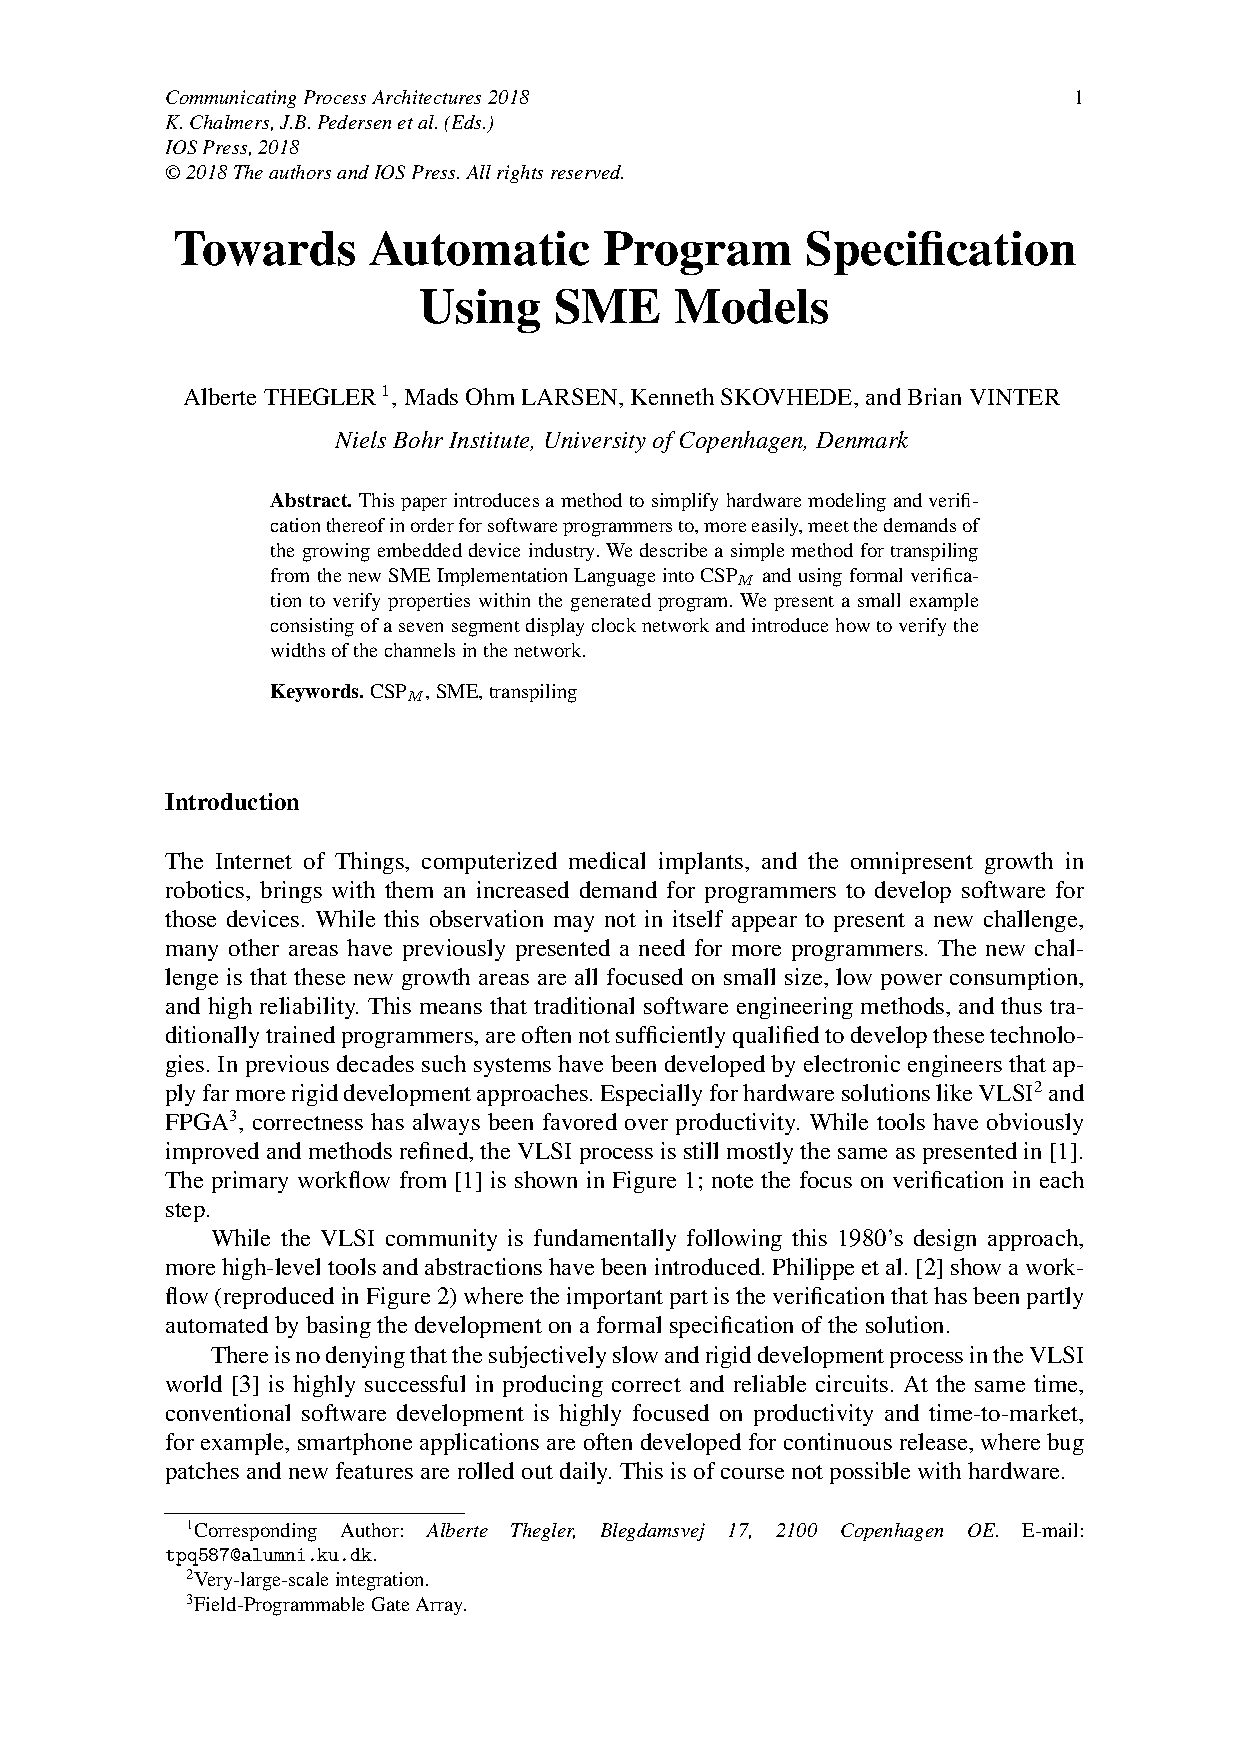
\includepdf[pages=-]{./paper/main.pdf}

\end{document}
